%-----------------------------------------
% To process this file:
%   pdflatex fpp-manual
%   biber fpp-manual
%   pdflatex fpp-manual
%   pdflatex fpp-manual
%-----------------------------------------

%\documentclass{article}
%
\documentclass{hitec}     % Tutorial overall style

\usepackage{biblatex}
\usepackage{index}
\usepackage{xr}
\usepackage{textgreek}
\usepackage{setspace}
\usepackage{graphicx}
\usepackage{moreverb}    % Defines {listing} environment.
\usepackage{amsmath, amsthm, amssymb, amsbsy, mathtools}
\usepackage{alltt}
\usepackage{rotating}
\usepackage{enumitem}
\usepackage{subcaption}
\usepackage{xspace}
\usepackage[section]{placeins}   % For preventing floats from floating to end of chapter.
\usepackage{longtable}  % For splitting long vertical tables into pieces
\usepackage{multirow}
\usepackage{booktabs}   % For table layouts
\usepackage{yhmath}     % For widehat
\usepackage{mathpazo}   % Make math equations look a bit bolder.
\usepackage{xcolor}     % Needed for listings package.
\usepackage{listings}
\usepackage[T1]{fontenc}   % so _, <, and > print correctly in text.
\usepackage[strings]{underscore}    % to use "_" in text
\usepackage[nottoc,numbib]{tocbibind}   % Makes "References" section show in table of contents
\usepackage[pdftex,colorlinks=true,bookmarksnumbered=true]{hyperref}   % Must be last package!
\usepackage{titletoc,tocloft}%
%%%%%%%%%%%%%$$$$$$$$$$$$$$$$$$$$$$$%%%%%%%%%%%%%%%% 
%%%%%%%%%%%%%%%%%%%%%%%%%%%%%%%%%%%%%%%%%%%%%%%%%%%
\addbibresource{bibliography.bib}

\setlength{\cftsubsecindent}{1cm}
\setlength{\cftsubsubsecindent}{2cm}
%\dottedcontents{section}[1.5em]{}{1.3em}{.6em}
%-------------------------------------------------------------------

\newcommand{\sref}[1]{\S\ref{#1}}
\newcommand{\Sref}[1]{Sec.~\sref{#1}}
\newcommand{\calO}{{\cal O}}
\newcommand{\Th}{$^{th}$\xspace}
\newcommand{\Eq}[1]{{Eq.~(\protect\ref{#1})}}
\newcommand{\Newline}{\hfil \\}

\newcommand{\vn}{\begingroup\catcode`\_=11 \catcode`\%=11 \dottcmd}
\newcommand\dottcmd[1]{{\usefont{T1}{lmss}{bx}{n} #1}\endgroup}

\newenvironment{example}
  {\vspace{-2.0ex} \begin{alltt}}
  {\end{alltt} \vspace{-1.5ex}}

\newcommand{\codefont}{\small}
\definecolor{light-gray}{gray}{0.95}
\lstset{backgroundcolor=\color{light-gray}}
\lstset{xleftmargin=0cm}
\lstset{framexleftmargin=0.3em}

\lstnewenvironment{Xcode}{}{}

\definecolor{lightcyan}{rgb}{0.88, 1.0, 1.0}
\newcounter{main}
\setcounter{main}{1}
\lstnewenvironment{code}[1][firstnumber=\themain,name=main]
  {\lstset{ %language=haskell,
           %columns=fullflexible,
           columns=fixed,
           basicstyle=\codefont\ttfamily,
           %numbers=left,
           numberstyle=\tiny\color{gray},
           backgroundcolor=\color{lightcyan},
           #1
          }
}
{\setcounter{main}{\value{lstnumber}}}



\definecolor{backcolor}{rgb}{0.8824,1.0,1.0}   % To match code environment
\definecolor{h}{rgb}{0.8824,0.3,0.3} 
\lstset{basicstyle = \small, backgroundcolor=\color{backcolor}, escapeinside = {@!}{!@}}

\renewcommand{\textfraction}{0.1}
\renewcommand{\topfraction}{1.0}
\renewcommand{\bottomfraction}{1.0}

\settextfraction{0.9}  % Width of text
\setlength{\parindent}{0pt}
\setlength{\parskip}{1ex}
%\setlength{\textwidth}{6in}
\newcommand{\Section}[1]{\section{#1}\vspace*{-1ex}}

\newenvironment{display}
  {\vspace*{-1.5ex} \begin{alltt}}
  {\end{alltt} \vspace*{-1.0ex}}

%%% Table of Contents spacing.
\makeatletter
\renewcommand{\l@section}{\@dottedtocline{1}{1.5em}{3.3em}}
\renewcommand{\l@subsection}{\@dottedtocline{2}{3.8em}{4.2em}}
\renewcommand{\l@figure}{\@dottedtocline{1}{1.5em}{3.3em}}
\renewcommand{\l@table}{\@dottedtocline{1}{1.5em}{3.3em}}
\makeatother


\def\ta{http://www.takafumi.org/etienne/new_pages/simple_programs/}
\def\tb{http://www.takafumi.org/etienne/new_pages/maps/}
\def\tc{http://www.takafumi.org/etienne/new_pages/programs/}
\def\td{http://www.takafumi.org/etienne/new_pages/universal_taylor/}
 
\def\tdemo{http://www.takafumi.org/etienne/new_pages/my_demo_package/}

\newcounter{mytable}
\Alph{mytable}
\def\smytable{\refstepcounter{mytable}\themytable}
%\newcommand\smytable[1][]{\refstepcounter{mytable}\label{#1}\themytable }
%\refstepcounter{foo}
%--------------------------------------------------------------------------------------------------------

\title{Fully Polymorphic Package Manual}

\author{}
\date{
  \parbox{6in}{
\includegraphics[width=5in]{logo-fpp.pdf}\vspace*{0.4in}} \\ 
  Etienne Forest and David Sagan \\ 
  March 25, 2023
}
 
%--------------------------------------------------------------------------------------------------------
\begin{document}
 
\phantomsection
\pdfbookmark[1]{Cover Page}{Cover Page}
%\maketitle

\cleardoublepage
\phantomsection
\pdfbookmark[1]{Contents}{Contents}
\tableofcontents

\newpage

%--------------------------------------------------------------------------------------------------------
\Section{Introduction to packages within FPP/PTC}
\label{s:intro}

The name PTC is commenly used to designate a code written by Etienne Forest with the help of Frank Schmidt and later David Sagan. PTC is an object oriented, open source, subroutine library for
\begin{itemize}
\item The manipulation and analysis of Taylor series and Taylor maps.
\item Modeling of charged particle beams in accelerators using Taylor maps.
\end{itemize}
The popularity of PTC can be attested to by its use with the Bmad\cite{b:bmad} toolkit for
accelerator and X-ray simulations as well as its use within the MAD\cite{b:mad} simulation program.

PTC is linked with the overloaded Truncated Power Series
Algebra (TPSA) package of Martin Berz. Berz's package is called \vn{Polymorphic Package} (PP). By
virtue of using the polymorphic package and by virtue of being able to do tracking, PTC stands for
``Polymorphic Tracking Code''. PTC is can be decomposed into two parts:
\begin{enumerate}
%
\item The Fully Polymorphic Package (FPP) part handles Taylor series.
FPP is pure mathematics detached from any "physics". 
%
\item The Tracking Code (TC) part is where the physics of PTC is located. It is simply an integrator pushing the phase space and spin of particles through magnets. 
TC relies on FPP for handling Taylor series. In particular,
via the magic of FPP (specifically the magic of PP), a Taylor map can be produced if wanted when tracking with TC.
%
\end{enumerate}

FPP is the subject of this manual. FPP itself can be subdivided into two parts:
\begin{enumerate}
\item\label{it:fpp} The ``Polymorphic Package'' (the PP of FPP) deals with the production of Taylor series.
\item\label{it:ap} The Analysis Package (AP) analyses physically sensible Taylors maps: Taylor maps that approximate the tracking of the code. Spin and magnet modulation can also be analyzed.
\end{enumerate}

To appreciate the role of PP, we can show a tiny piece of code  TC representing a drift.
\begin{code}
                      .
                      .
                      .
    TYPE(REAL_8),INTENT(INOUT):: X(6)
    TYPE(REAL_8),INTENT(IN):: L
                      .
                      .
                      .
          PZ=SQRT(1.0_dp+2.0_dp*X(5)/b+x(5)**2-X(2)**2-X(4)**2)
          X(1)=X(1)+L*X(2)/PZ
          X(3)=X(3)+L*X(4)/PZ
\end{code}         
 
 For completeness, here is  type \vn{real_8}:
 
 \begin{code}
   TYPE REAL_8
     TYPE (TAYLOR) T      !  USED IF TAYLOR
     REAL(DP) R           !    USED IF REAL
     INTEGER KIND  !  0,1,2,3 (1=REAL,2=TAYLOR,3=TAYLOR KNOB, 0=SPECIAL)
     INTEGER I   !   USED FOR KNOBS AND SPECIAL KIND=0
     REAL(DP) S   !   SCALING FOR KNOBS AND SPECIAL KIND=0
     LOGICAL(lp) :: ALLOC  ! IF TAYLOR IS ALLOCATED IN DA-PACKAGE
  END TYPE REAL_8
 \end{code}
 
In the above definition, we see \vn{real_8%t}
 and \vn{real_8%r}.  
 They are respectively the Taylor and double precision entries of the polymorph. If the polymorph must for some reason become a Taylor series, then its value is stored in \vn{%t}, otherwise it is stored in  \vn{%r}.   
  A \vn{real_8}  can also be a ``knob'': this is described in section (\sref{s:rc8}).
 
 
If  type \vn{REAL_8} was simply \vn{real(8)}, then this code fragment would simply be the exact formula for a drift in canonical variables. However \vn{REAL_8} can become a Taylor series in certain chosen variables at execution time and thus Taylor series can be produced. The actual package that does the Taylor calculation is the package of Martin Berz\cite{b:berz.da}
, namely the old version from LBNL properly modified by Johan Bengtson and overloaded by Etienne Forest using Fortran90.
 



% The FPP/PTC library has two parts. The Fully Polymorphic Package (FPP) is the part that deals with  Taylor series and maps. FPP is pure mathematics detached from any "physics".  The Polymorphic Tracking Code (PTC) part deals with the modeling of particle beams and accelerators. PTC contains the "physics" and relies on FPP for producing and manipulating Taylor maps.  This is illustrated in Figure~\ref{f:ptc}. Roughly, FPP can be subdivided into two parts, a Taylor manipulation part for basic manipulations of Taylor series and an analysis part to do things like normal form analysis. PTC uses the Taylor manipulation part of FPP for things like the construction of Taylor maps. Additionally, PTC uses the analysis tools of FPP. A closer look at FPP shows the existence of a Differential Algebra (DA) package within FPP. This package was originally coded by  Martin Berz.\cite{b:berz.da}



This manual is focused on how to use FPP. Since FPP is designed to serve PTC or a code like PTC, there will be some
mention of PTC but only so far as how PTC relates to FPP. In particular, tracking through lattices
is not discussed and the reader is referred to the PTC documentation for this.

\begin{figure}[tb]
  \centering
  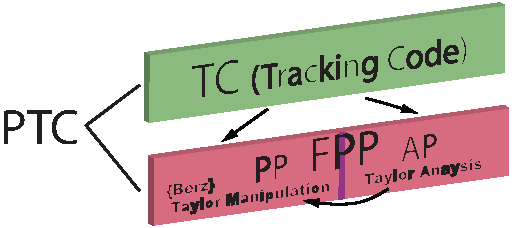
\includegraphics[width=0.9\textwidth]{ptcfppe.pdf}
  \caption{
The Fully Polymorphic Package (FPP) part of the FPP/PTC library provides manipulation and analysis
of Taylor series and maps and the Tracking Code (TC) part contains the physics of 
 the  accelerators. Arrows indicate code dependencies. The Taylor analysis code uses
the Taylor manipulation code but not vice versa. FPP does not use PTC but PTC code uses both FPP's
Taylor manipulation and potentially analysis as the red arrow indicates.
  }
  \label{f:ptc}
\end{figure}

The red arrow in Figure~\ref{f:ptc} refers to a potential dependency. PTC can dump on files Taylor series which can be analyzed or tracked by another code. Conversely, PTC (via FPP), can read maps produced by other codes and track them. For example, a person might have a COSY-INFINITY version of a damping ring and the subsequent injection line. The Taylor map describing this structure can be an input to PTC in the absence of a PTC lattice for this structure: this is equivalent to inputting linear uncoupled lattice functions in a regular code but much more general.


In fact most analysis in PTC in done by people (including the authors) who write independent modules for generalized Twiss calculations. This will be illustrated later and is the main topic of reference \cite{thenewbook}.


The FPP package can be used with any  tracking code including TC. Indeed one can  write an integrator in Fortran90 using the polymorphic types of FPP for the production and analysis of Taylor maps: Forest has written many such examples in lectures.



%--------------------------------------------------------------------------------------------------------
\Section{Where to Obtain FPP/PTC}
\label{s:obtain}

FPP/PTC can be downloaded from the web via the Bmad web site\cite{b:bmad} or at
\begin{code}
https://github.com/jceepf/fpp_book
\end{code}

Taylor manipulation routines are contained in the following code files:
\begin{code}
a_scratch_size.f90                j_tpsalie.f90           
b_da_arrays_all.f90               k_tpsalie_analysis.f90
b_da_arrays_all_pancake.f90       l_complex_taylor.f90    
c_dabnew.f90                      m_real_polymorph.f90    
c_dabnew_pancake.f90              n_complex_polymorph.f90
d_lielib.f90                      o_tree_element.f90      
h_definition.f90                  Sa_extend_poly.f90     
i_tpsa.f90
\end{code}

Taylor analysis routines are contained in the following code files
\begin{code}
cb_da_arrays_all.f90               Ci_tpsa.f90
cc_dabnew.f90                      Su_duan_zhe_map.f90
\end{code}

{\color{h}
The library 
\begin{code}
             Su_duan_zhe_map.f90
\end{code}
can actually be used separately. It allows for   tracking using Taylor maps: remember that PTC proper (TC) does not use Taylor maps for tracking, it is a ``kick code'' or integrator.}
%--------------------------------------------------------------------------------------------------------
\Section{Concepts: Taylor series, polymorphs and Taylor maps}
\label{s:concepts}

The purpose of this section is to explain why we would like to write an integrator equipped with polymorphism. Of course the purpose exists before the code and, for the most part, is not the result of ``Darwinian evolution''. 


 It is true from a goal driven point of view (teleological) that PTC was created with  the production of Taylor maps of phase space in mind. This is simply because Forest is convinced, see references \cite{thebook} and \cite{thenewbook}, that an analytical theory primarily based on finite ``s'' maps is superior than a theory primarily based on the  s-dependent Hamiltonian of the Courant-Snyder theory in the context of accelerators. This s-dependent Hamiltonian is far from the code and thus not adequate as the primary theory for most applications. 
 
 But can we guess from TC's structure, the tracking part, that PTC prioritizes  a map-based theory for analysis? The answer as we will see is :no.
 
 There are two options if we have Taylor maps in mind: 
 
 \begin{enumerate}
 \item We can write a beam line code whose goal is the production of Taylor series approximate maps around some chosen orbit and whose internal structure reflects this goal. 
 The prime representative of such codes is COSY-INFINITY\cite{cosy9,cosynim}. This is also true of MARYLIE,  TRANSPORT\cite{slac75} and the Twiss modules part of MAD8 ported into  MAD-X. All these codes choose a ``design'' orbit and then compute Taylor maps around this orbit. If a user examine these codes, especially  TRANSPORT, Taylor series maps will jump in their faces: arrays of monomial coefficients for each phase space variables are defined and they contain increasingly complex  formulae as the degree increases. The TRANSPORT approach reached a grotesque end point with the code COSY 5.0
 \footnote{This is not to be confused with COSY-INFINITY which uses Berz's TPSA package. COSY 5.0\cite{cosy5ham} was really the end of the dinosaur line of TRANSPORT like codes. It is mercifully extinct.}
% 
 of Berz : Fortran formulae at the fifth order Taylor coefficients covered pages of computer generated algebra.
 \item
 Forest, following mainly the philosophy of Talman, prefers the usage of integrators, in particular, symplectic integrator in the simulations of LINACs, recirculators and rings. (See Forest's review article \cite{forestreview} for a comprehensive opinionated description of this topic.)  As a result, and irrespective of teleological consideration i.e., wanting Taylor maps for analysis--Twiss, etc\ldots, TC  is a (mostly symplectic) integrator whose main purpose is the tracking of rays. It is only via polymorphism that this integrator can, under some very specific conditions, produce a Taylor map which approximates the phase space maps produced by the likes of COSY-INFINITY or MARYLIE.
  \end{enumerate}
  
 In fact Forest produced a ``kick code''. Imagine if the type \vn{real_8} was a Fortran90 intrinsic. Anyone could write a kick code using the floating point \vn{real(8)}. The fact that same person could recompile the code using \vn{real_8} would not automatically elevate the code to a code which produces sensible phase space maps. COSY-INFINITY, MARYLIE or TRANSPORT on the other hand always produce sensible maps when applied to magnets: this is their end purpose and their internal structure can be guessed from their purpose.

 Looking internally at TC, it is not possible to see any maps \footnote{A now retired CERN scientist exclaimed upon looking in the guts of PTC: ``where are the beta functions?'' The reader should understand upon reading this manual that this question  is ridiculous: they are nowhere. PTC is unaware of them even when it tracks them! This is the central topic of reference \cite{thenewbook}.}: only tracking of \vn{real_8} completely mimicking the tracking of \vn{real(8)}.
 
 
Therefore it  is not mathematically true that PTC produces ``Taylor maps'' despite Forest's motives. Sometimes PTC produces Taylor series and it is not clear to the author of PTC (Forest) what kind of maps should be created. An example of this is provided in sections (\sref{s:exttay}) and (\sref{s:lagmap}): from the Taylors series produced by PTC we construct a contracting map to be used in a Newton search. In that case, the user must write the interface since no one can guess {\it a priori} what the user has in mind.

 We will see that PTC provides an interface between TC and AP which privileges the production of phase space maps so that the users can {\it de facto} state that for the most part PTC facilitates the production of Taylor maps related to phase space via the derived type \vn{real_8}. But this is not visible in TC proper and is only true because Forest has programmed a very specific interface between polymorphs and Taylor maps. He could have left that task to the user (Bmad and MAD-X programmers) but they would have complained. Forest himself as the prime user would have complained schizophrenically to himself.
 
 



In the rest of this section we explain TC's interaction with FPP.  It is thus necessary to introduce certain concepts in very broad terms. Since PTC is an existing code, we can use its existing structures to describe the general approach. Someone else, writing in a different language would most likely be tempted to use similar concepts and perhaps do a better job.

After general considerations to set the tone and provide some context, we will examine 3 cases in section (\sref{s:tracking.analysis}):

 \begin{enumerate}
 \item In section (\sref{s:extmap}), we extract a phase space map.  We use special constructs  and routines  that facilitates this for the user. Namely they connect TC to AP. In AP, normal forms for example have very special assumptions : they deal with linearly stable spin-orbit maps for example.
 \item\label{itemla} In sections (\sref{s:exttay}) and (\sref{s:lagmap}), we create a contraction map that fits the output of TC  that has no connection with accelerator theory proper. FPP is used directly without the interface to AP. This program can be understood without the slightest understanding of TC and what it allegedly computes.
 \item In  section (\sref{s:lagmapt}), we fit the orbit (as in item \ref{itemla}) and the tunes/phase-slip. This is a typical accelerator physics case. We create the usual one-turn maps as well as the Langrangian contraction maps of item \ref{itemla}.
 \end{enumerate}
%-------------------------------------------------------------------
\subsection{Conventions}
\label{s:conventions}

FPP/PTC is written in Fortran90. It is assumed that the reader has some familiarity with this
language. In particular, it is assumed that the reader knows what a \vn{structure} is (roughly
corresponding to a \vn{class} in Python or C++) which is also called a \vn{derived type}. Additionally it is
assumed that the reader knows about operator overloading.

FPP/PTC uses double precision numbers. The kind type parameter ``\vn{dp}'' is defined in FPP/PTC to
correspond to double precision numbers.    For example:
\begin{code}
real(dp) abc, xyz             ! Declare double precision vars abc and xyz.
xyz = 3.4_dp * abc / 1e9_dp   ! 3.4_dp and 1e9_dp are double precision.
\end{code}

In this manual, \vn{real(dp)} is often written as \vn{real(8)} in case the meaning of \vn{dp} is forgotten. However \vn{dp} could be \vn{16} if quadruple precision is used.

\subsection{Some useful operators on Taylor series}\label{s:useful}

This section contains simple operations which are useful mainly to programmers using FPP.

 It must be remarked that the integral operator \vn{.i.} loses one order in the taylor series. It is better to use the \vn{c_universal_taylor} if integrals are needed to obtained Poisson bracket operators.

\setcounter{mytable}{0}
{\footnotesize
\begin{center}
\begin{tabular}{|l|c|c|}
\hline
 & Description (t: c_taylor) & Fortran Operator \\ \hline
\multirow{3}{*}{ \refstepcounter{mytable}\label{t:1}\themytable}
 & & \\
 & Real and imaginary part of c_taylor       & t=real(t) and t= aimag(t)  \\
  & & \\
 \hline
\multirow{3}{*}{\smytable}
 & & \\
 & Extract the coefficient of $x_i$  (constructing matrices)  & r=t.index.i \\
  & & \\
 \hline
\multirow{3}{*}{\smytable}
 & & \\
 & ${dt \over d{x}_{i}}$ and  $\int_{}^{}t\ d{x}_{i}$  & \href{\ta z_deriv.f90}{t=t.d.i } and \href{\ta z_deriv.f90}{t=t.i.i } \\
  & & \\
 \hline
\multirow{3}{*}{\smytable}
 & & \\
 & Extract  order ``i''  & \href{\ta z_sub_i.f90}{t=t.sub.i } \\
  & & \\
 \hline

\multirow{3}{*}{ \refstepcounter{mytable} \themytable}
 & & \\
 & Truncates above ``i''  & \href{\ta z_cut_sub.f90}{m=m.cut.i } \\
  & & \\
 \hline

\multirow{3}{*}{\smytable}
 & & \\
 & Extracts  coefficient $r$ of  monomials $\ {x}_{1}^{{j}_{1}}\cdots{x}_{1}^{{j}_{nv}}$ & \href{\ta z_sub_j.f90}{r=t.sub.j or r=t.sub.j}   \\
  & & \\
 \hline

\multirow{3}{*}{\smytable}
 & & \\
 &
 t=a + b $x_i$ where a and b are real or complex
& %
\href{\ta z_var.f90}{t=a+b dz_c(i)} 
 \\
  & & \\
 \hline



\multirow{3}{*}{\smytable}
 & & \\
 &Create Monomials 
%
%
%]|Expr|[#b @`b___})## b'4" Helvetica|: ;bP8&c0!*,D[#! (&"!*|:!r|
%| $^x^1^$^j^1_'b M$^x^1^$^j(!nv}_: }(%:!r $^x^1^$^j^1_'b M$^x^|
%|1^$^j(!nv}_}(#r $^x^i_}}: ,D}& b!( b"0 b#8 b$@ b%H b&P!WW}]|[
$\begin{array}{ccc}r\ {x}_{1}^{{j}_{1}}\cdots{x}_{1}^{{j}_{nv}}\\
r\ {x}_{1}^{{j}_{1}}\cdots{x}_{1}^{{j}_{nv}}\\
r\ {x}_{i}\end{array}$


& %
%]|Expr|[#b @`b___})## b'4" Helvetica|: ;bP8&c0!*,D[#! (?-[-<rm|
%| -<href-[-<ta z-?sub-?i,Nf90-]-[t,]r,Ncmono,Nj,H1,Znv,I-] -]}|
%|(?-[-<rm -<href-[-<ta z-?sub-?i,Nf90-]-[t,]r,Ncmono,Nj,H1,Znv|
%|,I-] -]}(?-[-<rm -<href-[-<ta z-?sub-?i,Nf90-]-[t,]r,Ncmono,N|
%|j,H1,Znv,I-] -]}},D}& b!( b"0 b#8 b$@ b%H b&P!WW}]|[
$\begin{array}{ccc}{\rm \href{\ta z_sub_i.f90}{t=r.cmono.j(1:nv)} }\\
{\rm \href{\ta z_mono.f90}{t=r.cmono.'j1...jnv'} }\\
{\rm \href{\ta z_mono.f90}{t=r.cmono.i} }\end{array}$
 \\
  & & \\
 \hline
\multirow{3}{*}{ \refstepcounter{mytable}\label{t:par}\themytable}
 & & \\ &
Peek coefficient $t$ , as a c_taylor, of monomial %
%]|Expr|[#b @`b___})%# b'4" Helvetica|: ;bP8&c0!*,D$^"!*|:!x^1|
%|^$^j^1_'b M$^x^n^$^j^n_: ,D}& b!( b"0 b#8 b$@ b%H b&P!WW}]|[
${x}_{1}^{{j}_{1}}\cdots{x}_{n}^{{j}_{n}}$
& %
 %
%]|Expr|[#b @`b___})## b'4" Helvetica|: ;bP8&c0!*,D["! (=-[-<rm|
%| -<href-[-<ta z-?par,Nf90-]-[t,]r,Npar,Nj,H1,Znv,I-] -]}(<-[-<|
%|rm -<href-[-<ta z-?par,Nf90-]-[t,]r,Npar,N,Gj1,N,N,Njn,G -]-]}}|
%|,D}& b!( b"0 b#8 b$@ b%H b&P!WW}]|[
$\begin{array}{cc}{\rm \href{\ta z_par.f90}{t=r.par.j(1:nv)} }\\
{\rm \href{\ta z_par.f90}{t=r.par.'j1...jn' }}\end{array}$
 \\
  & & \\
 \hline
\multirow{3}{*}{\smytable}
 & & \\
 &
Generalization of .par. using a type called sub_taylor (inf)
& %
\href{\ta z_parT.f90}{t=r.par.inf or t=r.part.inf } 
 \\
  & & \\
 \hline
\multirow{3}{*}{ \refstepcounter{mytable}\label{t:shift}\themytable}
 & & \\
 &
Shift exponents downwards by k
& %
\href{\ta z_shift.f90}{t=t<=k} 
 \\
  & & \\
 \hline
\multirow{3}{*}{\smytable}
 & & \\
 &
 Peek and shift (operators \ref{t:par} and \ref{t:shift}  combined)
& %
\href{\ta z_shift.f90}{t=t<=k} 
 \\
  & & \\
 \hline
\multirow{3}{*}{\smytable}
 & & \\
 &
	Pseudo derivative  : %
$d({x}_{i}^{n})={x}_{i}^{n-1}$

& %
\href{\ta z_pseudo_deriv.f90}{t=t.k.i} 
 \\
  & & \\
 \hline
\multirow{3}{*}{\smytable}
 & & \\
 &
Poisson Bracket

& %
\href{\ta z_poisson.f90}{t=t.pb.t'} 
 \\
  & & \\
 \hline
\end{tabular}
\end{center}
 }

\subsection{Some useful operators on c_damap and c_vector_field  }\label{s:usefulmap}


\setcounter{mytable}{0}
{\footnotesize
\begin{center}
\begin{tabular}{|l|c|c|}
\hline
 & Description  (M,A: c_damap and F,F': c_vector_field %
%]|Expr|[#b @`b___})%# b'4" Helvetica|: ;bP8&c0!*,DF"!Symbol^:!&c0  /7|
%|/1: &c0!*,D}& b!( b"0 b#8 b$@ b%H b&P!WW}]|[
$F\cdot \nabla $
)& Fortran Operator \\ \hline
\multirow{3}{*}{ \refstepcounter{mytable} \themytable}
 & & \\
 & Extract  order ``i''  & \href{\tb z_cut_sub.f90}{M=M.sub.i } \\
  & & \\
 \hline
\multirow{3}{*}{ \refstepcounter{mytable} \themytable}
 & & \\
 & Truncates above ``i''  & \href{\tb z_cut_sub.f90}{M=M.cut.i } \\
  & & \\
 \hline
\multirow{3}{*}{ \refstepcounter{mytable} \themytable}
 & & \\
 & Extracts  order ``i''  & \href{\tb z_vf_cut_sub.f90}{F=F.sub.i } \\
  & & \\
 \hline
\multirow{3}{*}{ \refstepcounter{mytable} \themytable}
 & & \\
 & Truncates above ``i''  & \href{\tb z_vf_cut_sub.f90}{F=F.cut.i } \\
  & & \\
 \hline
\multirow{3}{*}{ \refstepcounter{mytable} \themytable}
 & & \\
 & Exponenting a vector field & \href{\tb z_vf_cut_sub.f90}{M=exp(F,M) or M=exp(F)} \\
  & & \\
 \hline
\multirow{3}{*}{ \refstepcounter{mytable} \themytable}
 & & \\
 & Logarithm of a map (look at link for optional variables) & \href{\tb z_vf_cut_sub.f90}{F=ln(M)} \\
  & & \\
 \hline
\multirow{3}{*}{ \refstepcounter{mytable}\label{t1:vect}\themytable}
 & 
%
%]|Expr|[#b @`b___})## b'4" Helvetica|: ;bP8&c0!*,D["" (."!Chicago^:!A|
%|<c!$1()""Times|:"F"#Symbol^:#&c0  /7/1"$*|:$&c0!*,K: -<hat-[:$f|
%|: -]}}$^:!A_(": ,M1},]:$ <c$4Q^F}:#&c0  /7/1:$&c0!*,K: -<hat-[|
%|<c$4Q^:$f}: -]}_(%:!A:$,]: -<exp<c!$1(%$^:$F^a_:#&c0  /7/1:$&c0!*,K|
%|$^q^:#&c0  a_}}}_}: &c0!*,D}& b!( b"0 b#8 b$@ b%H b&P!WW}]|[
$\begin{array}{cc}{\cal A}\left({F\cdot \nabla +\hat{f}}\right){{\cal A}}^{-1}=\ \widetilde{F}\cdot \nabla +\hat{\widetilde{f}}&\\
{\cal A}=
\exp\left({{F}_{a}\cdot \nabla +{q}_{\alpha }}\right)&\end{array}$

%
%]|Expr|[#b @`b___})## b'4" Helvetica|: ;bP8&c0!*,D[#" )%# b'4|
%|$^<c$4Q^"!*|:!F}^k_: ,]<c!$1(#$^:!F^i_$^""Symbol^:"&c0  .V^:!&c0!*i|
%|_$^a^k(",M1}}}:"&c0  .P:!&c0!*a}& b!( b"0 b#8 b$@ b%H b&P!WW}|
%|_),# b'4<c$4Q^: f} ,]<c!$1(#$^<c$4Q^:!F}^k_$^:"&c0  .V^:!&c0!*k|
%|_$^:"&c0  a_(":!&c0!*,M1}}}:"&c0  a:!&c0!*,K$^:"&c0  a_(":!&c0!*,M|
%|1}f:"&c0  .P:!&c0!*a :"&c0  a}& b!( b"0 b#8 b$@ b%H b&P!WW}_(4|
%|:!&c0!*a"#Monaco^:# is the orbital map and :"&c0  a:#&c0!* is|
%| the quaternion:! }_}: ,D}& b!( b"0 b#8 b$@ b%H b&P!WW}]|[
$\begin{array}{cc}{\widetilde{F}}_{k}=\left({{F}_{i}{\partial }_{i}{a}_{k}^{-1}}\right)\circ a&\\
\widetilde{f} =\left({{\widetilde{F}}_{k}{\partial }_{k}{\alpha }^{-1}}\right)\alpha +{\alpha }^{-1}f\circ a\ \alpha &\\
a~{\rm i}{\rm s}~{\rm t}{\rm h}{\rm e}~{\rm o}{\rm r}{\rm b}{\rm i}{\rm t}{\rm a}{\rm l}~{\rm m}{\rm a}{\rm p}~{\rm a}{\rm n}{\rm d} ~\alpha ~{\rm i}{\rm s}~{\rm t}{\rm h}{\rm e}~{\rm q}{\rm u}{\rm a}{\rm t}{\rm e}{\rm r}{\rm n}{\rm i}{\rm o}{\rm n}\ &\end{array}$
& \href{\tb z_vf_Lie_sub.f90}{F=A*F}
\\
  & & \\
 \hline
\multirow{3}{*}{ \refstepcounter{mytable} \themytable}
 & & \\
 & If $\cal A = $exp(F'$\cdot \nabla$) in item \ref {t1:vect}& \href{\tb z_vf_Lie_sub.f90}{F=exp_ad( F',F)}\\
  & & \\
 \hline
\multirow{3}{*}{ \refstepcounter{mytable} \themytable}
 & & \\
 & Lie Bracket: exp_ad reprogrammed with .lb. & \href{\tb z_vf_Lie_sub.f90}{F=F.lb.F}\\
  & & \\
 \hline
\multirow{3}{*}{ \refstepcounter{mytable} \themytable}
 & & \\
 & Tpsa and DA concatenation of \vn{c_damap}'s and powers (see \sref{s:datpsamaps})& %
%
%]|Expr|[#b @`b___})3# b'4" Helvetica|: ;bP8&c0!*,D-<href-[-<tc|
%| z-?track-?da-?tpsa,Nf90-]-[["" )1# b'4M,]A,No,NM,L M,]M,Noo,N,H|
%|n,I}& b!( b"0 b#8 b$@ b%H b&P!WW}_)-# b'4M,]A,N,J,NM,L M,]M,N,J,J,N,H|
%|n,I}& b!( b"0 b#8 b$@ b%H b&P!WW}_} -],D|
%|}& b!( b"0 b#8 b$@ b%H b&P!WW}]|[
$\href{\tb z_track_da_tpsa.f90}{\begin{array}{cc}M=A.o.M, M=M.oo.(n)&\\
M=A.*.M, M=M.**.(n)&\end{array} }$

\\
  & & \\
 \hline
\multirow{3}{*}{ \refstepcounter{mytable} \themytable}
 & & \\
 & M+M',M-M', r*M (r is real or complex) & \href{\tb z_simple_operations.f90}{M=A*M  and M=M**(n)}\\
  & & \\
 \hline

\end{tabular}
\end{center}

 }

\subsection{The type c_universal_taylor }\label{s:cuniversal}


A taylor series produced by TC or a map analysed by FPP depends on the two versions of the TPSA package of Berz. One version deals intrinsically with real Taylor: this is \vn{c_dabnew.f90}. It is the package on which the polymorphs are used and therefore used by the code TC.  A complex taylor does exist but simply made of two real taylors
\begin{code}
  type complextaylor
     type (taylor) r  ! Real part
     type (taylor) i  ! Imaginary part
  end type complextaylor
\end{code}
and similarily a complex polymorph exists and it is used in TC and it uses the above \hbox{\vn{complextaylor}}:
\begin{code}
  type complex_8
     type (complextaylor) t
     complex(dp) r
     logical(lp) alloc
     integer kind
     integer i,j
     complex(dp) s
   end type complex_8
\end{code}

The other package, \vn{cc_dabnew.f90} is a version of Berz package which is intrisically complex. It is used in the analysis part of FPP namely \vn{Ci_tpsa.f90}. During a run of PTC or worse BMAD, we would like to store permanently some Taylor series.  This is not possible via Berz's package since they function with a given order and number of variables. For that purpose BMAD uses a type  \vn{universal_taylor} and AP uses the complex equivalent \vn{c_universal_taylor}. Since this manual is about analysis --- not BMAD--- we describe  the \vn{c_universal_taylor} via examples in a table.


\setcounter{mytable}{0}
{\footnotesize
\begin{center}
\begin{tabular}{|l|c|c|}
\hline
 & \mbox{\footnotesize   (t,f: c_taylor, M,A: c_damap and F,F': c_vector_field, uf,uf1: c_universal_taylor )}& Fortran Operator \\ \hline
\multirow{3}{*}{ \refstepcounter{mytable}\label{t3:1}\themytable}
 & & \\
 & \mbox{\scriptsize Simple operations illustrated via a one-resoance normal form }&
 \href{\td z_uni.f90}{ \mbox{\scriptsize .sub.~.par.~.d.}} \\
  & & \\
 \hline
\multirow{3}{*}{ \refstepcounter{mytable}\label{t3:2}\themytable}
 & & \\
 & \mbox{\scriptsize Multiplicity of logarithms of maps and unversal taylors for Poisson brackets }& \href{\td z_vector_field_poisson.f90}{ \mbox{\scriptsize  get_field_c_universal_taylor(vf,uf1)}} \\
  & & \\
 \hline
\multirow{3}{*}{ \refstepcounter{mytable}\label{t3:3}\themytable}
 & & \\
 & \mbox{\scriptsize Evaluation via .o. on c_universal_taylor(:) }&
 \href{\td z_uni.f90}{ \mbox{\scriptsize uf.o.c_ray and uf(:).o.c_ray}} \\
  & & \\
 \hline
\end{tabular}
\end{center}

 }


In item \ref{t3:2}, we compute the logarithm of map two different ways: via \vn{ln(c_damap)} and normal form. The logarithm can only be used on map near the identity.  Via the normal form, it is easy to generate an infinite number of logarithms for maps far from the identity by simply adding integer units of tune to the linear tune.

In item  \ref{t3:3}, we substitute a type \vn{c_ray} into a inversal taylor or an array. An array can represent a map for example: not fast by very convenient. The type c_ray is:

\renewcommand{\codefont}{\footnotesize}
\begin{code}
 type c_ray
  complex(dp) x(lnv)            ! orbital and/or PTC magnet modulation clocks
  type(complex_quaternion) q    ! quaternion
  integer n                     ! of dimensions used in x(lnv)
!  Obsolescent
  complex(dp) s1(3),s2(3),s3(3) !# 3 spin directions
 end type c_ray
\end{code}
\renewcommand{\codefont}{\small}

If a \vn{c_ray}  is used with a \vn{c_damap}, the quaternion array will be filled with the resulting quaternion.


%-------------------------------------------------------------------
\subsection{TPSA Versus DA}
\label{s:tpsa}

TPSA stands for ``Truncated Power Series Algebra'' and DA stands for ``Differential Algebra.''
What does it mean when applied to a typical accelerator ring? Once we cut the mathematical jargon,
we will see that

\begin{itemize}
\item TPSA operations take into account the constant part and the results change as a function of the order (see below). 
%
\item DA operations are equivalent to normal TPSA operations used around the closed orbit and thus the
constant part of the map is ignored. All the coefficients of the Taylor series stay the same
independently of the order invoked. It so happens that the computation of nonlinear differential
operators (Lie vector fields for example), are self-consistent because they form a differential
algebra. But it is much simpler in our field to state that they are self-consistent because there
are no feed down terms.
\end{itemize}

It is important to understand why a non-zero constant part of a Taylor series can be
problematical. To see this, consider two TPSA maps of order $N$. One maps $x$ to $y$ and the second
maps $y$ to $z$:
\begin{align}
  y &= \sum_{j = 0}^N a_j x^j  \label{yj0n} \\
  z &= \sum_{j = 0}^N b_j y^j + \calO(y^{N+1}) \label{zj0n}
\end{align}
In \Eq{zj0n} it is made explicit that there are terms of order $N+1$ or higher that are being neglected.
The two maps can be concatenated to form a map of {\color{h}$w$ as a function of $x$:
\begin{equation}
  w\left({x}\right) = \sum_{j = 0}^N c_j x^j
  %
%]|Expr|[#b @`b___})## b'4" Symbol^: ;bP8&c0  .Z"!*|:!&c0!*z<c!$1|
%|("y<c!$1^x}}}}& b!( b"0 b#8 b$@ b%H b&P!WW}]|[
\equiv z\left({y\left({x}\right)}\right)
  \label{zj0nc}
\end{equation}
}
If there is a neglected term in \Eq{zj0n} that looks, for example, like $b_m y^m$ with $m > N$, substituting
\Eq{yj0n} into this term will result in modification of all lower order terms in \Eq{zj0nc} if, and
only if, $a_0$ is non-zero. This is
called ``feed-down''. That is, terms of higher order will affect the coefficients of lower order
terms when TPSA maps are combined. To avoid this, maps with zero constant term (DA maps) should be used. With
simulations, this generally means computing maps with respect to the   orbit. For
lattices with a closed geometry, this generally means computing maps with respect to the {\color{h} actual period-one closed} 
orbit. For lattices with an open geometry (EG: Linacs), the reference orbit can be some orbit
defined by tracking a beam from some {\color{h} wisely } user-specified initial position.

%-------------------------------------------------------------------
\subsection{Polymorphism}
\label{s:poly}

In computer programming ``\vn{polymorphism}'' is the property that a given variable, object, or
function can act in different ways depending upon the context. With FPP/PTC, polymorphism is used to
define types that can act as if the structure components were real valued numbers or Taylor series.
See the documentation of the \vn{real_8} type (\sref{s:real.8}) as an example.

Note: Many \vn{PTC} tracking code routines come in pairs. One routine of the pair, typically having a 
``r'' suffix in its name, will use real variables while the other routine, typically having a ``p'' suffix 
in its name. {\color{h} One could track real numbers with the polymorphic routines but this with entail a substantial speed decrease and therefore we opted for a duplication of the routines.}

Polymorphic types always have structure names that have a \vn{_8}
suffix.

%-------------------------------------------------------------------
\subsection{Operator Overloading}
\label{s:overloading}

FPP/PTC heavily uses operator overloading for  the manipulation of Taylor series  and polymorphs. Not only are the standard
arithmetical operators ($+, -, *, /, **$) overloaded as well as the equal sign ($=$), but there are
a number of custom operators that are defined as well. Below is a partial list.\footnote
  {\color{h}
Note: Fortran mandates that custom operator names begin and end with a dot ``.''. These operators have the lowest priority and therefore require parentheses. The usual Fortran operators, if overloaded, inherit the priorities of the intrinsic operators. 
  }
\begin{description}
\item[+, -] \Newline
Standard addition and subtraction of Taylor series.
%
\item[*] \Newline
$M1 * M2$ is used with two maps for  {\color{h} a DA concatenation while  $M1 \rm{.o.} M2$ is a TPSA concatenation with constant part retained.}
%
\item[.o.] \Newline

\item[**] \Newline   Powers of Taylor maps

\item[.oo.] \Newline Powers of Taylor maps using .o. for concatenation.

\end{description}

The difference between \vn{.o.} and \vn{*} was explained in section (\sref{s:datpsamaps}) using a one-dimensional example for simplicity.  

\subsection{Tracking Versus Analysis}
\label{s:tracking.analysis}

An important distinction here is the difference between \vn{tracking} and \vn{analysis}. By
``tracking'' it is meant  the propagation through a lattice of a single particle {\color{h} which typically 
involves six \vn{real_8} numbers for the orbital motion and four \vn{real_8}  for spin represented via a quaternion.}

{\color{h} However,  with  objects ending in  \vn{_8}, the orbital part and the quaternion can   internally become Taylor series in some variables via polymorphism.
{\it De facto}, if these polymorphs are properly initialized, then we can end up tracking Taylor series which can be turned into {\it bona fide} Taylor maps which approximate the beam line as they do in COSY-INFINITY or MARYLIE. Typically this is used to either compute a one-turn Taylor map or propagate a 
canonical transformation such as the Courant-Snyder transformation. However it could also produce a map unrelated to the usual one-turn map, for example, the closed orbit as a Taylor series in  dipole strengths or anything \ldots}
 \footnote
  {
Mathematically, single particle tracking is just tracking  using Taylor series
truncated at zeroth order. From the code perspective, due to the speed reduction with dealing with
Taylor series, the two are distinct: the routines with suffixes \vn{_r} and \vn{_p}.
  }
This is opposed to ``analysis'' which is the study of a {\color{h} Taylor} transport map to extract such things as
tunes, lattice functions, resonance driving terms, etc. With \vn{FPP}, analysis is always done on  {\color{h} Taylor}  maps.

\subsection{TC tracks elements of the algebra $\prescript{}{no}{D}_{nv}$
}
\label{s:tpsadef}

The purpose of this section is to unpack clearly the statement that PTC can track Taylor maps while TC tracks polymorphs which are members of an algebraic extensions of the real numbers. We do this with examples because in the end, all of this is very trivial if we focus on applications rather than theory. For the theory, the reader can look at Berz's book \cite{theberzbook} and in particular  the section on Levi-Civita fields\footnote{We think that it is better for most readers to get a practical view of Berz's idea before reading his exposition of such fields.} which provide inverses to the infinitesimals.

Since any function is a map, we usually reserve the word map to a function of phase space which, in TC, is of dimension 2 at a minimum. Therefore when PTC invokes TPSA it will always track Taylor ``maps'' but they can be nonsensical as a beam line map. We do  allow PTC  to track without any TPSA monomials reserved for the orbital motion, but this is only  permitted if the TPSA package is initialized with a subroutine proper to FPP: it forces the programmer to view TC as  just  an ``unknown'' black box subroutine. We will see what it implies  in section (\sref{s:exttay}).


Mathematically what does TC track?

A normal ``kick'' code tracks a subset of the field $(\mathbb{R},+,\times)$, namely floating point numbers. When embedded in the code Bmad, the TC subroutine ``\vn{propagate}'' , which we will encounter in the examples, is a function (or map in the usual mathematical sense) from :
%
%]|Expr|[#b @`b___})b P# b'4" Chicago^: ;bP8&c0!*-="!Helvetica|:! |
%|$('-[-<mathbb-[R-]-]}_^6""Times|:" :!,F-<stackrel-[TC-]-[-<longmapsto|
%|-]:"  $(':!-[-<mathbb-[R-]-]}_^6"#Symbol^:# :!-<-<:# :! z ,F-<|
%|longrightarrow $^z_^f,]TC,Hz,I:# :!-<-<"$Monaco^:$ where  in |
%|Bmad  "%*|:%z:!,F:%,]<c!$1(3x,L$^p^x_,O$^p^0_,Ly,L$^p^y_,O$^p|
%|^0_,L:#&c0  b:%&c0!*ct,L:#&c0  d:%&c0!*p,O$^p^0_}}:#&c0  /., |
%|$(':!&c0!*-[-<mathbb-[R-]-]}_^6:#&c0  : &c0!*-;|
%|}& b!( b"0 b#8 b$@ b%H b&P!WW}]|[
\begin{align} {{\mathbb{R}}}^{6}\ &\stackrel{TC}{\longmapsto}\ \ {{\mathbb{R}}}^{6} \\  z &\longrightarrow {z}^{f}=TC(z) \\~{\rm w}{\rm h}{\rm e}{\rm r}{\rm e}~~{\rm i}{\rm n}~{\rm B}{\rm M}{\rm A}{\rm D}~~z&=
\left({x,{P}_{x}/{p}_{0},y,{P}_{y}/{p}_{0},\beta ct,\delta P/{p}_{0}}\right)\in {{\mathbb{R}}}^{6}\end{align}


PTC or \vn{propagate}  is a map of  ${{\mathbb{R}}}^{6}$ in PTC at a minimum. (Spin and other goodies can be included).

Polymorphism extends $(\mathbb{R},+,\times)$ to an algebra called by Berz\cite{theberzbook} ~$\prescript{}{no}{D}_{nv} $, i.e., to $(\prescript{}{no}{D}_{nv} ,+,\times )$. This is the TPSA algebra described in  \sref{s:tpsa}. This algebra is a ring, not a field, i.e., not all elements have inverses. In fact all the so-called infinitesimals have no inverses. Colloquially, we might say that we deal with Taylor series not Laurent series. Thus we can say very clearly that 
%
%]|Expr|[#b @`b___})b R# b'4" Chicago^: ;bP8&c0!*-="!Helvetica|:! |
%| $(.-<prescript-[-]-[no-]-[D-]-?-[nv-]}_^6""Times|:"  :!,F-<stackrel|
%|-[TC-]-[-<longmapsto-]:"  $(.:!-<prescript-[-]-[no-]-[D-]-?-[|
%|nv-]}_^6 "#Symbol^:# :!-<-<:# :! z ,F-<longrightarrow $^z_^f,]|
%|TC,Hz,I:# : ;8/<"$*|:$;bP8eq,Zptcmap: ;8/=:!;bP8-<-<"%Monaco^:% |
%|where :$z:!,F:$,]<c!$1(3x,L$^p^x_,O$^p^0_,Ly,L$^p^y_,O$^p^0_,L|
%|:#&c0  b:$&c0!*ct,L:#&c0  d:$&c0!*p,O$^p^0_}}:#&c0  /.:$&c0!* |
%|$(.:!-<prescript-[-]-[no-]-[D-]-?-[nv-]}_^6: -;|
%|}& b!( b"0 b#8 b$@ b%H b&P!WW}]|[
\begin{align}  {\prescript{}{no}{D}_{nv}}^{6}\ \ &\stackrel{TC}{\longmapsto}\ \ {\prescript{}{no}{D}_{nv}}^{6}  \\  z &\longrightarrow {z}^{f}=TC(z) \label{eq:ptcmap}\\~{\rm w}{\rm h}{\rm e}{\rm r}{\rm e}~z&=
\left({x,{p}_{x}/{p}_{0},y,{p}_{y}/{p}_{0},\beta ct,\delta p/{p}_{0}}\right)\in \ {\prescript{}{no}{D}_{nv}}^{6}\end{align}

As an example, we can use a 1-d example as in \Eq{eq:m1t0}. Consider  two second order polynomials in one-variable, i.e., elements of $\prescript{}{2}{D}_{1}$:
%
%]|Expr|[#b @`b___})b K# b'4" Chicago^: ;bP8&c0!*-="!Monaco^:! |
%|if   ""Times|:"m"#Helvetica|:#,F,]$^"$*|:$m^0_,K$^m^1_"%Symbol^:%&c0  D|
%|:$&c0!*,K$^m^2_$^:%&c0  D_^:$&c0!*2   : ;bP;/":#;bP8 :!and   |
%|:$n:#,F,]$^:$n^0_,K$^n^1_:%&c0  D:$&c0!*,K$^n^2_$^:%&c0  D_^:$&c0!*2|
%|    : ;8/<:$;bP8eq,Znodnv: ;8/=;bP8-;}& b!( b"0 b#8 b$@ b%H b&P!WW}]|[
\begin{align}~{\rm i}{\rm f}~~~m&={m}_{0}+{m}_{1}\Delta +{m}_{2}{\Delta }^{2}\ \ \ \nonumber \\
 {\rm a}{\rm n}{\rm d} ~~~n&={n}_{0}+{n}_{1}\Delta +{n}_{2}{\Delta }^{2}\ \ \ \ \label{eq:nodnv}\end{align}
then we can write
%
%]|Expr|[#b @`b___})b O# b'4" Chicago^: ;bP8&c0!*-="!Monaco^:! |
%|if   ""Times|:"m"#Helvetica|:#,F"$Symbol^:$&c0  .Z<c!$1(%$^"%*|:%&c0!*m|
%|^0_,L$^m^1_,L$^m^2_}}:$&c0  /.:#&c0!*-<prescript-[-]-[2-]-[D-]-?-[|
%|1-]: ;bP;/":#;bP8 :!and   :%n:#,F:$&c0  .Z<c!$1(%$^:%&c0!*n^0|
%|_,L$^n^1_,L$^n^2_}}:$&c0  /.:#&c0!*-<prescript-[-]-[2-]-[D-]-?-[|
%|1-]: ;8/<:%;bP8eq,Znodnv1: ;8/=;bP8-;}& b!( b"0 b#8 b$@ b%H b&P!WW}]|[
\begin{align}~{\rm i}{\rm f}~~~m&\equiv \left({{m}_{0},{m}_{1},{m}_{2}}\right)\in \prescript{}{2}{D}_{1}\nonumber \\
 {\rm a}{\rm n}{\rm d} ~~~n&\equiv \left({{n}_{0},{n}_{1},{n}_{2}}\right)\in \prescript{}{2}{D}_{1}\label{eq:nodnv1}\end{align}
%
 In \Eq{eq:nodnv1}, we use the array notation for elements of the ring $\prescript{}{2}{D}_{1}$ which is more in line with the actual Fortran90 code.
Then we have:
%
%]|Expr|[#b @`b___})-# b'4" Chicago^: ;bP8&c0!*-="!Times|:!m.Q|
%|n""Helvetica|:",F,]<c!$1).# b'4$^"#*|:#m^0_:!&c0  .Q$^:#&c0!*n|
%|^0_,L$^m^1_:!&c0  .Q$^:#&c0!*n^1_,L$^m^2_:!&c0  .Q$^:#&c0!*n^|
%|2_}& b!( b"0 b#8 b$@ b%H b&P!WW}} : ;8/<:#;bP8eq,Znodnvpm: ;8/=|
%|;bP8-;}& b!( b"0 b#8 b$@ b%H b&P!WW}]|[
\begin{align}m\pm n&=\left({{m}_{0}\pm {n}_{0},{m}_{1}\pm {n}_{1},{m}_{2}\pm {n}_{2}}\right)\ \label{eq:nodnvpm}\end{align}
and for multiplication,
%
%]|Expr|[#b @`b___})-# b'4" Chicago^: ;bP8&c0!*-="!Times|:!m""Symbol^:"&c0  .T|
%|:!&c0!*n"#Helvetica|:#,F,]<c!$1)1# b'4$^"$*|:$m^0_$^n^0_,L$^m|
%|^0_$^n^1_,K$^m^1_$^n^0_,L$^m^2_$^n^0_,K$^m^1_$^n^1_,K$^m^0_$^|
%|n^2_}& b!( b"0 b#8 b$@ b%H b&P!WW}} : ;8/<:$;bP8eq,Znodnvpmul|
%|: ;8/=;bP8-;}& b!( b"0 b#8 b$@ b%H b&P!WW}]|[
\begin{align}m\times n&=\left({{m}_{0}{n}_{0},{m}_{0}{n}_{1}+{m}_{1}{n}_{0},{m}_{2}{n}_{0}+{m}_{1}{n}_{1}+{m}_{0}{n}_{2}}\right)\ \label{eq:nodnvpmul}\end{align}
and finally for division we have,
%
%]|Expr|[#b @`b___})-# b'4" Chicago^: ;bP8&c0!*-="!Times|:!m""Symbol^:"&c0  .X|
%|:!&c0!*n"#Helvetica|:#,F,]<c!$1)%# b'4<2^$^"$*|:$m^0_)!# b'4$|
%|^n^0_}& b!( b"0 b#8 b$@ b%H b&P!WW}},L,M<2(%$^m^0_$^n^1_,M$^m|
%|^1_$^n^0_})!# b'4$^n^0^2}& b!( b"0 b#8 b$@ b%H b&P!WW}},L,M<2|
%|(-$^m^0_$^n^0_$^n^2_,M$^m^0_$^n^1^2,K$^m^1_$^n^0_$^n^1_,M$^m^|
%|2_$^n^0^2})!# b'4$^n^0^3}& b!( b"0 b#8 b$@ b%H b&P!WW}}|
%|}& b!( b"0 b#8 b$@ b%H b&P!WW}} : ;8/<:$;bP8eq,Znodnvpdiv: ;8/=|
%|;bP8-;}& b!( b"0 b#8 b$@ b%H b&P!WW}]|[
\begin{align}m\div n&=\left({{{m}_{0} \over {n}_{0}},-{{m}_{0}{n}_{1}-{m}_{1}{n}_{0} \over {n}_{0}^{2}},-{{m}_{0}{n}_{0}{n}_{2}-{m}_{0}{n}_{1}^{2}+{m}_{1}{n}_{0}{n}_{1}-{m}_{2}{n}_{0}^{2} \over {n}_{0}^{3}}}\right)\ \label{eq:nodnvpdiv}\end{align}

It should be clear from this example that we regain the field of real (or complex) numbers if only the entry of the element of $\prescript{}{2}{D}_{1}$ is used. Secondly, if $n_0 = 0$, then the division of \Eq{eq:nodnvpdiv} is not defined: we have a ring, not a scalar field (See Berz\cite{theberzbook}).


When  TC tracks elements of $ \prescript{}{no}{D}_{nv} $, it is totally ``unaware'' that these objects can be turned into {\it bona fide} phase space Taylor maps: this was shown in the drift code fragment of section (\sref{s:intro}) where no ``Taylor maps'' are to be seen. In  
order to explain this dichotomy between tracking and analysis, between polymorphs and Taylors maps, we need to  define  different structures of FPP/PTC that
are optimized to handle one or the other. 
Structures that have been designed to handle tracking are
\begin{code}
TC structures

real_8
complex_8    (only used internally in TC)
probe_8
probe    (this is the real version of probe_8)
\end{code}

and for analysis here is an important subset  

\begin{code}
AP structures

c_taylor
c_damap
c_normal_form
c_vector_field
\end{code}

Finally we have structures which allow us to save Taylor series outside the TPSA package(s) of Berz. This is a permanent kind of storage that does not depend
on the order and number of variables used by the TPSA of Berz which underpins FPP. They are totally independent.
\begin{code}
Storage structures

universal_taylor
c_universal_taylor
\end{code}

While the structures that PTC uses for tracking are discussed here, the details of how to track through
a lattice are deferred to the PTC documentation. Here the primary concern is FPP and analysis as well as the interaction between analysis and tracking, between AP and TC.

 The interaction between the world of polymorphs \vn{_8}, which are elements of $\prescript{}{no}{D}_{nv} $ and Taylor maps, we will illustrate below in section (\sref{s:extmap}).
In summary, the code TC produces the usual orbital and spin but, via polymorphism, it can be fed into a structure \vn{c_damap}, which is a Taylor map and thus can be analyzed if sensible. The result of this analysis, for example a Courant-Snyder transformation, in the form of a \vn{c_damap}, can then be fed into a polymorphic ray (\vn{probe_8}, and tracked again. This is how one does any type of Twiss calculation, i.e., propagates canonical transformations including spin and nonlinearities. This is the topic of reference \cite{thenewbook}.

{\bf Nota Bene:}

In summary, there are 3 ways to look at a TPSA variable. They are all isomorphic mathematically but they serve very different purposes in the human brain.

\begin{enumerate}
\item As a polynomial in some variable, say $\Delta $ of \Eq{eq:nodnv}, with automatic truncation at order $no+1$. Our brains are in physics mode when doing this.
\item As a polynomial in some abstract object, say $\Delta $ of \Eq{eq:nodnv}, where  ${\Delta }^{no+1}=0$.  In that case we are dealing with an abstract representation of $\prescript{}{no}{D}_{nv} $.  This is useful when thinking about $(\prescript{}{no}{D}_{nv},+,\times )$. Our brains are in mathematical mode. 
\item\label{itemsp} Finally, the algebra $(\prescript{}{no}{D}_{nv},+,\times )$ can be represented as an n-tuple as in \Eq{eq:nodnv1}. Here we are in a computer science mode since ultimately the computer stores all the TPSA variables in arrays with specific rules under addition and multiplication. 
\end{enumerate}

Item \ref{itemsp} is fully demonstrated if one downloads from the git site the following folder:
\begin{code}
https://github.com/jceepf/fpp_book/my_demo_package
\end{code}
This folder contains a mini-TPSA and analysis package as well as a nonlinear Twiss example.


Indeed, the TSPA package of that site (no polymorph but only Taylor) contains the following definition of a Taylor derived type:


\begin{code}
 TYPE my_taylor             
    complex(dp) a(0:n_mono)    
END TYPE my_taylor
\end{code}

This package can represent  $(\prescript{}{0}{D}_{3},+,\times )$, $(\prescript{}{1}{D}_{3},+,\times )$, $(\prescript{}{2}{D}_{3},+,\times )$, $(\prescript{}{3}{D}_{3},+,\times )$ and $(\prescript{}{4}{D}_{3},+,\times )$. Obviously $(\prescript{}{0}{D}_{3},+,\times )$ is just the field of complex numbers $({\mathbb{C}},+,\times )$ where each number is stored \vn{my_taylor%a(0)}.

Moreover addition and subtraction  are defined respectively by overloading the Fortran90 intrinsic operators via the following functions:

\begin{code}
  FUNCTION add( S1, S2 )
    implicit none
    TYPE (my_taylor) add
    TYPE (my_taylor), INTENT (IN) :: S1, S2

     add%a=S1%a + S2%a     
     
     call clean(add)
  END FUNCTION add
  
  
  FUNCTION subs( S1, S2 )
    implicit none
    TYPE (my_taylor) subs
    TYPE (my_taylor), INTENT (IN) :: S1, S2

     subs%a=S1%a - S2%a     
     
     call clean(subs)
  END FUNCTION subs
  
  
 \end{code}

This is exactly \Eq{eq:nodnvpm}.  We encourage the reader to compile the files and run the main program. 


\section{DA and TPSA maps}\label{s:datpsamaps}

The code for this section is located at \href{\tc z_track_da_tpsa.f90}{\vn{z_track_da_tpsa.f90}}.

A code like TC always produces TPSA objects by default. To make the explanations simple, we will assume here  that TC is tracking for one turn in a ring. The closed orbit in that case is a natural special orbit demanded by theory. For example, all textbooks assume some version of Hill's equation {\bf around the  ideal closed orbit} when discussing Courant-Snyder theory.


Calling this orbit $f$ --- for fixed point --- we have: 
%
%]|Expr|[#b @`b___})0# b'4" Chicago^: ;bP8&c0!*-="!Helvetica|:! |
%|f,]TC,Hf,I : ;8/<""*|:";bP8eq,Zfixtc: ;8/=:!;bP8 : -;|
%|}& b!( b"0 b#8 b$@ b%H b&P!WW}]|[
\begin{align} f=TC(f) \label{eq:fixtc} \end{align}
%
We now, via polymorphism, track the following ray $z_0$:
%
%]|Expr|[#b @`b___}).# b'4" Chicago^: ;bP8&c0!*-="!Helvetica|:! |
%|$^""*|:"z^0_,]f,K"#Symbol^:#&c0  D:!&c0!* : ;8/<:";bP8eq,Zidtpsa|
%|: ;8/=;bP8-;}& b!( b"0 b#8 b$@ b%H b&P!WW}]|[
\begin{align} {z}_{0}=
f+\Delta  \label{eq:idtpsa}\end{align}
%
%
$\Delta $ is an array of infinitesimals:
%
%]|Expr|[#b @`b___})8# b'4" Chicago^: ;bP8&c0!*-="!Helvetica|:! |
%|""Symbol^:"&c0  D:!&c0!*,F,]<c!$1(%$^:"&c0  D^"#*|:#&c0!*1_,L|
%|'b M,L$^:"&c0  D(!:#&c0!*nv}_}}"$Monaco^:$     where   $^:"&c0  D|
%|^:#&c0!*k(#no,K1},]0:! : ;8/<:#;bP8eq,Znilpot: ;8/=;bP8-;|
%|}& b!( b"0 b#8 b$@ b%H b&P!WW}]|[
\begin{align} \Delta &=\left({{\Delta }_{1},\cdots,{\Delta }_{nv}}\right)~~~~~{\rm w}{\rm h}{\rm e}{\rm r}{\rm e}~~~{\Delta }_{k}^{no+1}=
0 \label{eq:nilpot}\end{align}
%
If we substitute \Eq{eq:idtpsa} in $TC(z)$, we get:
%
%]|Expr|[#b @`b___})b @# b'4" Chicago^: ;bP8&c0!*-="!Helvetica|:! |
%|TC,H""*|:"f,K"#Symbol^:#&c0  D:!&c0!*,I ,]TC,H:"f:!,I,K$^:"t^|
%|f_:!,H:#&c0  D:!&c0!*,I,]:"f,K$^t^f_:!,H:#&c0  D:!&c0!*,I : ;8/<|
%|:";bP8eq,Zfixtmap: ;8/=:!;bP8 : -;}& b!( b"0 b#8 b$@ b%H b&P!WW}]|[
\begin{align} TC(f+\Delta ) =TC(f)+{t}_{f}(\Delta )=f+{t}_{f}(\Delta ) \label{eq:fixtmap} \end{align}
%
${t}_{f}(\Delta )$ is a (vector) polynomial in $\Delta $ of maximum degree $no$ and such that ${t}_{f}(0)=0$

We can evaluate $TC$ at a different ray not involving the closed orbit $f$, for example, we can use some arbitrary input in the units of TC:

%
%]|Expr|[#b @`b___})b @# b'4" Chicago^: ;bP8&c0!*-="!Helvetica|:! |
%|TC,H""*|:"z,K"#Symbol^:#&c0  D:!&c0!*,I ,]TC,H:"z:!,I,K$^:"t^|
%|z_:!,H:#&c0  D:!&c0!*,I,]$^:"z^1_,K$^t^z_:!,H:#&c0  D:!&c0!*,I|
%| : ;8/<:";bP8eq,Zztmap: ;8/=:!;bP8 : -;|
%|}& b!( b"0 b#8 b$@ b%H b&P!WW}]|[
\begin{align} TC(z+\Delta ) =TC(z)+{t}_{z}(\Delta )={z}_{1}+{t}_{z}(\Delta ) \label{eq:ztmap} \end{align}


In \Eq{eq:fixtmap} and \Eq{eq:ztmap}, the variable $\Delta $ represents a different expansion. If we want $\Delta $ to represent  the same variable, we need to translate these expressions:
%
%]|Expr|[#b @`b___})b H# b'4" Chicago^: ;bP8&c0!*-="!Helvetica|:! |
%|$^""*|:"m^f_<c!$1^"#Symbol^:#&c0  D}:!&c0!*,]:"f,K$^t^f_:!,H:#&c0  D|
%|:"&c0!*,Mf:!,I"$Monaco^:$   and   $^:"m^z_<c!$1^:#&c0  D}:!&c0!*,]|
%|$^:"z^1_,K$^t^z_:!,H:#&c0  D:"&c0!*,Mz:!,I : ;8/<:";bP8eq,Zfixtmapf|
%|: ;8/=:!;bP8 : -;}& b!( b"0 b#8 b$@ b%H b&P!WW}]|[
\begin{align} {m}_{f}\left({\Delta }\right)=f+{t}_{f}(\Delta -f)~~~{\rm a}{\rm n}{\rm d} ~~~{m}_{z}\left({\Delta }\right)={z}_{1}+{t}_{z}(\Delta -z) \label{eq:fixtmapf} \end{align}


In \Eq{eq:fixtmapf}, the maps $m_f$ and $m_z$ are the same if and only if $no=\infty$.  For example, we have:
%
%]|Expr|[#b @`b___})9# b'4" Chicago^: ;bP8&c0!*-="!Helvetica|:! |
%|$^""*|:"m^f_<c!$1^f}:!,]:"f,]$^m^z_<c!$1^f} ,K O,H$^<c!1!(#z,M|
%|f}}_(#no,K1},I"#Monaco^:# :" : ;8/<:";bP8eq,Zfixtmapfe: ;8/=:!;bP8 |
%|: -;}& b!( b"0 b#8 b$@ b%H b&P!WW}]|[
\begin{align} {m}_{f}\left({f}\right)=f=
{m}_{z}\left({f}\right)\ +\ O({\left|{z-f}\right|}^{no+1})~\ \label{eq:fixtmapfe} \end{align}

\Eq{eq:fixtmapfe} is again exposing a symptom to TPSA maps: inconstant in the order ${no}$ is finite.

Next we see how to such maps can be concatenated.

\subsection{Concatenating two TPSA maps}\label{s:concattpsa}
 
 Consider two TPSA maps:
%
%]|Expr|[#b @`b___})b H# b'4" Chicago^: ;bP8&c0!*-="!Helvetica|:! |
%|$^""*|:"m)!# b'4$^w^0_}& b!( b"0 b#8 b$@ b%H b&P!WW}_<c!$1^z}|
%|:!,]$^:"w^1_,K$^M)!# b'4$^w^0_}& b!( b"0 b#8 b$@ b%H b&P!WW}_|
%|:!,H:"z,M$^w^0_:!,I"#Monaco^:#   and   $^:"n)!# b'4$^z^0_|
%|}& b!( b"0 b#8 b$@ b%H b&P!WW}_<c!$1^z}:!,]$^:"z^1_,K$^N)!# b'4|
%|$^z^0_}& b!( b"0 b#8 b$@ b%H b&P!WW}_:!,H:"z,M$^z^0_:!,I : ;8/<|
%|:";bP8eq,Zconcatt: ;8/=:!;bP8 :" : -;}& b!( b"0 b#8 b$@ b%H b&P!WW}]|[
\begin{align} {m}_{{w}_{0}}\left({z}\right)={w}_{1}+{M}_{{w}_{0}}(z-{w}_{0})~~~{\rm a}{\rm n}{\rm d} ~~~{n}_{{z}_{0}}\left({z}\right)={z}_{1}+{N}_{{z}_{0}}(z-{z}_{0}) \label{eq:concatt} \ \end{align}


For the record here, in FPP, the map ${m}_{{w}_{0}}$ of \Eq{eq:concatt} is stored as follows:

\vskip 0.2cm
{\color{blue}
\small
\hskip 1cm type(c_damap) m    | Here nv=nd2 + \# of parameters

\hskip 4cm  .

\hskip 1cm m\%x0(1:nd2)=$w_0$ \hskip 0.5cm | these are \vn{complex(dp)}, nd2 is the size of phase space

\vskip -1.2cm
%
%]|Expr|[#b @`b___}))# b'4" Chicago^: ;bP8&c0!*-="!Helvetica|:! |
%|: ;8/<""*|:";bP8eq,Zcdamap: ;8/=:!;bP8 : -;|
%|}& b!( b"0 b#8 b$@ b%H b&P!WW}]|[
\begin{align} \label{eq:cdamap} \end{align}

\hskip 1cm m\%v(1:nd2) = $w_1$(1:nd2)+$M_{w_0}(\Delta$(1:nv))   \hskip 0.5cm | these are complex Taylor, i.e., in Berz's $\prescript{}{no}{D}_{nv} $

 }
\vskip 0.2cm

We  compute now the map $t=m\circ n$:


%
%]|Expr|[#b @`b___})b T# b'4" Chicago^: ;bP8&c0!*-="!Times|:!t|
%|""Helvetica|:",F,]<c!$1(#$^"#*|:#m)!# b'4$^w^0_|
%|}& b!( b"0 b#8 b$@ b%H b&P!WW}_"$Symbol^:$&c0  .P$^:#&c0!*n)!# b'4|
%|$^z^0_}& b!( b"0 b#8 b$@ b%H b&P!WW}_}}<c!$1^:$&c0  D}: ;bP;&c0!*/"|
%|:";bP8 ,F,]$^:#w^1_,K$^M)!# b'4$^w^0_}& b!( b"0 b#8 b$@ b%H b&P!WW}|
%|_:",H$^:#n)!# b'4$^z^0_}& b!( b"0 b#8 b$@ b%H b&P!WW}_<c!$1^:$&c0  D}|
%|:#&c0!*,M$^w^0_:",I: ;bP;/":";bP8 ,F,]$^:#w^1_,K$^M)!# b'4$^w|
%|^0_}& b!( b"0 b#8 b$@ b%H b&P!WW}_:",H$^:#N)!# b'4$^z^0_|
%|}& b!( b"0 b#8 b$@ b%H b&P!WW}_:",H:$&c0  D:#&c0!*,M$^z^0_:",I,K|
%|$^:#z^1_,M$^w^0_:",I: ;bP;/":";bP8 ,F,]<c%"C^<cY A(($^:#w^1_,K|
%|$^M)!# b'4$^w^0_}& b!( b"0 b#8 b$@ b%H b&P!WW}_:",H$^:#z^1_,M|
%|$^w^0_,I}}^$^t^1__}:",K<c%"C^<cY A(#$^:#M)!# b'4$^w^0_|
%|}& b!( b"0 b#8 b$@ b%H b&P!WW}_:$&c0  .P$^:#&c0!*N)!# b'4$^z^|
%|0_}& b!( b"0 b#8 b$@ b%H b&P!WW}_}}^$^T^$^z^0__(#DA :$&c0  .P}}|
%|:"&c0!*,H:$&c0  D:#&c0!*,M$^z^0_:",I : ;8/<:#;bP8eq,Zconcattot|
%|: ;8/=;bP8-;}& b!( b"0 b#8 b$@ b%H b&P!WW}]|[
%

%
%]|Expr|[#b @`b___})b J# b'4" Chicago^: ;bP8&c0!*-="!Times|:!t|
%|<c!$1^""*|:"x}"#Helvetica|:#,F,]<c!$1(#$^:"m)!# b'4$^w^0_|
%|}& b!( b"0 b#8 b$@ b%H b&P!WW}_"$Symbol^:$&c0  .P$^:"&c0!*n)!# b'4|
%|$^z^0_}& b!( b"0 b#8 b$@ b%H b&P!WW}_}}<c!$1^x}: ;bP;/":#;bP8 |
%|,F,]$^:"w^1_,K$^M)!# b'4$^w^0_}& b!( b"0 b#8 b$@ b%H b&P!WW}_|
%|:#,H$^:"n)!# b'4$^z^0_}& b!( b"0 b#8 b$@ b%H b&P!WW}_<c!$1^x}|
%|,M$^w^0_:#,I: ;bP;/":#;bP8 ,F,]$^:"w^1_,K$^M)!# b'4$^w^0_|
%|}& b!( b"0 b#8 b$@ b%H b&P!WW}_:#,H$^:"N)!# b'4$^z^0_|
%|}& b!( b"0 b#8 b$@ b%H b&P!WW}_:#,H:"x,M$^z^0_:#,I,K$^:"z^1_,M|
%|$^w^0_:#,I:" : ;8/<:";bP8eq,Zconcattot: ;8/=;bP8-;|
%|}& b!( b"0 b#8 b$@ b%H b&P!WW}]|[
\begin{align}t\left({x}\right)&=\left({{m}_{{w}_{0}}\circ {n}_{{z}_{0}}}\right)\left({x}\right)\nonumber \\
 &={w}_{1}+{M}_{{w}_{0}}({n}_{{z}_{0}}\left({x}\right)-{w}_{0})\nonumber \\
 &={w}_{1}+{M}_{{w}_{0}}({N}_{{z}_{0}}(x-{z}_{0})+{z}_{1}-{w}_{0})\ \label{eq:concattot}\end{align}

This operation is done in FPP between two \vn{c_damap}'s using the operator \vn{.o.}

\subsection{Inverse of a TPSA map in terms of  a DA map }\label{s:inversetpsa}

The inverse of a DA map is well known. First one inverses the linear part, a matrix, and then one inverses the nonlinear part by an iterative method that has a finite number of steps, namely $no$ at most.  This routine was programmed by Berz and is in \vn{c_dabnew.f90}.  In FPP is called  as follows:

\begin{code}
type(c_damap) m, m_inverse
       .
       .
m_inverse= m**(-1)
       .
       .
\end{code}

We work out the TPSA inverse of ${m}_{{w}_{0}}$   of \Eq{eq:concatt}. To do so we solve the following equation for $y$ in terms of $x$:
%
%
%]|Expr|[#b @`b___})b M# b'4" Chicago^: ;bP8&c0!*-="!Helvetica|:! |
%|$^""*|:"m)!# b'4$^w^0_}& b!( b"0 b#8 b$@ b%H b&P!WW}_<c!$1^x}|
%|:!,]$^:"w^1_,K$^M)!# b'4$^w^0_}& b!( b"0 b#8 b$@ b%H b&P!WW}_|
%|:!,H:"x,M$^w^0_:!,I,]y"#Monaco^:# : ;bP;/":!;bP8 "$Symbol^:$&c0  />|
%|:"&c0!* x,]$^M)!# b'4$^w^0_}& b!( b"0 b#8 b$@ b%H b&P!WW}(",M|
%|1}<c!$1(#y,M$^w^1_}},K$^w^0_:# : ;bP;/":#;bP8 or  $^:"m)!# b'4|
%|$^w^0_}& b!( b"0 b#8 b$@ b%H b&P!WW}(",M1}<c!$1^x},]$^M)!# b'4|
%|$^w^0_}& b!( b"0 b#8 b$@ b%H b&P!WW}(",M1}<c!$1(#x,M$^w^1_}},K|
%|$^w^0_: ;8/<:";bP8eq,Ztpsainv: ;8/=:!;bP8 : -;|
%|}& b!( b"0 b#8 b$@ b%H b&P!WW}]|[
\begin{align} {m}_{{w}_{0}}\left({x}\right)={w}_{1}+{M}_{{w}_{0}}(x-{w}_{0})=y~\nonumber \\
 \Rightarrow \ x=
{M}_{{w}_{0}}^{-1}\left({y-{w}_{1}}\right)+{w}_{0}~\nonumber \\
~{\rm o}{\rm r}~~{m}_{{w}_{0}}^{-1}\left({x}\right)=
{M}_{{w}_{0}}^{-1}\left({x-{w}_{1}}\right)+{w}_{0}\label{eq:tpsainv} \end{align}


In FPP, the TPSA inverse is invoked by the following call:

\begin{code}
type(c_damap) m, m_tpsa_inverse
       .
       .
m_tpsa_inverse= m.oo.(-1)
       .
       .
\end{code}



\subsection{Concatenating two DA maps using their TPSA representation}\label{s:concatda}

In a ``DA'' situation, the exit value of the first map must be the entrance value of the second map,i.e., they must be evaluated on the same orbit. Therefore we must have  ${z}_{1}={w}_{0}$:
%
%]|Expr|[#b @`b___})b G# b'4" Chicago^: ;bP8&c0!*-="!Helvetica|:! |
%|$^""*|:"m)!# b'4$^w^0_}& b!( b"0 b#8 b$@ b%H b&P!WW}_<c!$1^"#Symbol^:#&c0  D}|
%|:!&c0!*,]$^:"w^1_,K$^M)!# b'4$^w^0_}& b!( b"0 b#8 b$@ b%H b&P!WW}|
%|_:!,H:#&c0  D:"&c0!*,M$^w^0_:!,I"$Monaco^:$   and   $^:"n)!# b'4|
%|$^z^0_}& b!( b"0 b#8 b$@ b%H b&P!WW}_<c!$1^:#&c0  D}:!&c0!*,]|
%|$^:"w^0_,K$^N)!# b'4$^z^0_}& b!( b"0 b#8 b$@ b%H b&P!WW}_:!,H|
%|:#&c0  D:"&c0!*,M$^z^0_:!,I : ;8/<:";bP8eq,Zdadatpsa: ;8/=:!;bP8 |
%|: -;}& b!( b"0 b#8 b$@ b%H b&P!WW}]|[
\begin{align} {m}_{{w}_{0}}\left({\Delta }\right)={w}_{1}+{M}_{{w}_{0}}(\Delta -{w}_{0})~~~{\rm a}{\rm n}{\rm d} ~~~{n}_{{z}_{0}}\left({\Delta }\right)={w}_{0}+{N}_{{z}_{0}}(\Delta -{z}_{0}) \label{eq:dadatpsa} \end{align}

For example the first map could be from the entrance of a wiggler to its center followed by the second half of the wiggler. Obviously, the exit value of ${n}_{{z}_{0}}$ must be the entrance value of the ray of map  ${m}_{{w}_{0}}$.  Here we verified, that in this case, we can ignore completely these constant values. In an integrator, this happens completely naturally since we do not deal with \vn{c_damap} but with the rays themselves in polymorphic form, i.e., type \vn{probe_8}. 

%
%]|Expr|[#b @`b___})b P# b'4" Chicago^: ;bP8&c0!*-="!Helvetica|:! |
%|<c!$1(#$^""*|:"m)!# b'4$^w^0_}& b!( b"0 b#8 b$@ b%H b&P!WW}_"#Symbol^:#&c0  .P|
%|$^:"&c0!*n)!# b'4$^z^0_}& b!( b"0 b#8 b$@ b%H b&P!WW}_}}<c!$1|
%|^:#&c0  D}:!&c0!*,F,]$^:"w^1_,K$^M)!# b'4$^w^0_|
%|}& b!( b"0 b#8 b$@ b%H b&P!WW}_:!,H$^:"n)!# b'4$^z^0_|
%|}& b!( b"0 b#8 b$@ b%H b&P!WW}_<c!$1^:#&c0  D}:"&c0!*,M$^w^0_|
%|:!,I: ;bP;/":!;bP8 ,F,]$^:"w^1_,K$^M)!# b'4$^w^0_|
%|}& b!( b"0 b#8 b$@ b%H b&P!WW}_:!,H$^:"N)!# b'4$^z^0_|
%|}& b!( b"0 b#8 b$@ b%H b&P!WW}_:!,H:#&c0  D:"&c0!*,M$^z^0_:!,I,I|
%|: ;bP;/":!;bP8 ,F,]$^:"w^1_,K<c!$1()$^M)!# b'4$^w^0_|
%|}& b!( b"0 b#8 b$@ b%H b&P!WW}_:#&c0  .P$^:"&c0!*N)!# b'4$^z^|
%|0_}& b!( b"0 b#8 b$@ b%H b&P!WW}_:#&c0  .P:!&c0!*,H:"I,M$^z^0|
%|_:!,I}}<c!$1^:#&c0  D}:!&c0!* : ;bP;/":!;bP8 ,F,]$^:"w^1_,K<c%"C|
%|^<cY A^<c!$1(#$^M)!# b'4$^w^0_}& b!( b"0 b#8 b$@ b%H b&P!WW}_|
%|:#&c0  .P$^:"&c0!*N)!# b'4$^z^0_}& b!( b"0 b#8 b$@ b%H b&P!WW}|
%|_}}}_(#DA :#&c0  .P}}<c!$1($D, :"&c0!*,M$^z^0_:#&c0  }}: ;8&c0!*/<|
%|:";bP8eq,Zconcatda: ;8/=;bP8-;}& b!( b"0 b#8 b$@ b%H b&P!WW}]|[
\begin{align} \left({{m}_{{w}_{0}}\circ {n}_{{z}_{0}}}\right)\left({\Delta }\right)&={w}_{1}+{M}_{{w}_{0}}({n}_{{z}_{0}}\left({\Delta }\right)-{w}_{0})\nonumber \\
 &={w}_{1}+{M}_{{w}_{0}}({N}_{{z}_{0}}(\Delta -{z}_{0}))\nonumber \\
 &={w}_{1}+\left({{M}_{{w}_{0}}\circ {N}_{{z}_{0}}\circ (I-{z}_{0})}\right)\left({\Delta }\right) \nonumber \\
 &={w}_{1}+\underbrace{\left({{M}_{{w}_{0}}\circ {N}_{{z}_{0}}}\right)}\limits_{}^{DA\ \circ }\left({\Delta -{z}_{0}}\right)\label{eq:concatda}\end{align}


We see in \Eq{eq:concatda},  where $I-{z}_{0}$ represents a translation,  that only the concatenation of the map around the orbit is necessary, i.e., %
%
%]|Expr|[#b @`b___}(%" Helvetica|: ;bP8&c0!*,D$^"!*|:!M)!# b'4|
%|$^w^0_}& b!( b"0 b#8 b$@ b%H b&P!WW}_""Symbol^:"&c0  .P$^:!&c0!*N|
%|)!# b'4$^z^0_}& b!( b"0 b#8 b$@ b%H b&P!WW}_: ,D}]|[
${M}_{{w}_{0}}\circ {N}_{{z}_{0}}$. This is why, in FPP, the DA concatenation does not keep track of the constant parts at all. This is the case, for example, during all the normal form operations:   in the linear case for example, all the  the matrices are  around the closed orbit, no feed-down effects are present and thus constant parts can be ignored in diagonalizing the matrix.


This DA operation is done in FPP between two \vn{c_damap}'s using the operator \vn{*}.

\subsubsection{Where are  TPSA map and DA stored: one two Fortran type but two operations}\label{s:storage}

A code like TC naturally produces TPSA maps of the form
%
%]|Expr|[#b @`b___}):# b'4" Chicago^: ;bP8&c0!*-="!Times|:!TC,H|
%|z,I,]$^""*|:"m)!# b'4$^w^0_}& b!( b"0 b#8 b$@ b%H b&P!WW}_<c!$1|
%|^z}"#Helvetica|:#,]$^:"w^1_,K$^M)!# b'4$^w^0_|
%|}& b!( b"0 b#8 b$@ b%H b&P!WW}_:#,H:"z,M$^w^0_:#,I"$Monaco^:$ |
%|  : ;8/<:";bP8eq,Ztpsamap: ;8/=:#;bP8 : -;|
%|}& b!( b"0 b#8 b$@ b%H b&P!WW}]|[
\begin{align}TC(z)=
{m}_{{w}_{0}}\left({z}\right)={w}_{1}+{M}_{{w}_{0}}(z-{w}_{0})~~~\label{eq:tpsamap} \end{align}
%
%
This map is produced by tracking a particle starting at  ${w}_{0}$ and using TPSA to extract the Taylor representation denoted by ${M}_{{w}_{0}}$.  However there is an infinite number of choices for $w_0$:
%
%]|Expr|[#b @`b___}).# b'4" Chicago^: ;bP8&c0!*-="!Times|:!TPSA|
%|,]$^<c!(A($$^""*|:"w^0_"#Symbol^:#&c0  /.$(%"$Helvetica|:$&c0!*-<|
%|mathbb-[R-]}_^6<c!0!(0:"TC,Hz,I,]$^m)!# b'4$^w^0_|
%|}& b!( b"0 b#8 b$@ b%H b&P!WW}_<c!$1^z}:$,]$^:"w^1_,K$^M)!# b'4|
%|$^w^0_}& b!( b"0 b#8 b$@ b%H b&P!WW}_:$,H:"z,M$^w^0_:$,I}}}}(#|
%|:"No,]:#&c0  .E}_"%Monaco^:%&c0!*   : ;8/<:";bP8eq,Ztpsamapd: ;8/=|
%|:$;bP8 : -;}& b!( b"0 b#8 b$@ b%H b&P!WW}]|[
\begin{align}TPSA=
{\left\{{{w}_{0}\in {\mathbb{R}}^{6}\left|{TC(z)=
{m}_{{w}_{0}}\left({z}\right)={w}_{1}+{M}_{{w}_{0}}(z-{w}_{0})}\right.}\right\}}_{No=
\infty }~~~\label{eq:tpsamapd} \end{align}

If the order $No$ is infinite, then all these maps are identical and anyone could be used to represent the map of the code, namely $TC(z)$. You are simply expanding the same function around a different point.

In fact their Taylor representations form a natural equivalent class. Things start to degenerate if $No$ is finite, as it is in all realistic applications:
%
%]|Expr|[#b @`b___}).# b'4" Chicago^: ;bP8&c0!*-=$(!"!Times|:!TPSA}|
%|(!No}_,]$^<c!(A($$^""*|:"w^0_"#Symbol^:#&c0  /.$(%"$Helvetica|:$&c0!*-<|
%|mathbb-[R-]}_^6<c!0!(0:"TC,Hz,I:#&c0  .[$^:"&c0!*m)!# b'4$^w^|
%|0_}& b!( b"0 b#8 b$@ b%H b&P!WW}_<c!$1^z}:$,]$^:"w^1_,K$^M)!# b'4|
%|$^w^0_}& b!( b"0 b#8 b$@ b%H b&P!WW}_:$,H:"z,M$^w^0_:$,I}}}}(#|
%|:"No,\:#&c0  .E}_"%Monaco^:%&c0!*   : ;8/<:";bP8eq,Ztpsamapda|
%|: ;8/=:$;bP8 : -;}& b!( b"0 b#8 b$@ b%H b&P!WW}]|[
\begin{align}{TPSA}_{No}=
{\left\{{{w}_{0}\in {\mathbb{R}}^{6}\left|{TC(z)\approx {m}_{{w}_{0}}\left({z}\right)={w}_{1}+{M}_{{w}_{0}}(z-{w}_{0})}\right.}\right\}}_{No<\infty }~~~\label{eq:tpsamapda} \end{align}

With a finite $No$, there is a need to be close to the design orbit (LINAC) or closed orbit (ring). This is to avoid feed down issues. This is achieved, in a ring, by choosing the map expressed around the actual closed orbit of the code TC.

It is clear that any member of that set can be stored to order $No$ in the type \vn{c_damap}. Therefore we use this type for both DA and TPSA maps.

 The difference is in the operator used: both are types \vn{c_damap}. If \vn{M} and \vn{N} are DA maps, then the resulting DA map \vn{K} will be:

\begin{code}
K=M*N
\end{code}

If we intend \vn{M} and \vn{N} to be TPSA maps, then the code is

\begin{code}
K=M.o.N
\end{code}

The code for \vn{M*N} completely ignore the constant parts when performing the required substitutions. For example, in a linear map, we are just multiplying matrices.

As we will see in section (\sref{s:exampletpsa}) ), $w_0$ is stored in \vn{c_damap%x0(:)}. It is ignored by the DA concatanation ``$*$''.

\subsection{Finding the closed orbit of  a one-turn TPSA map}\label{s:fixtpsa}

In an integrator such as Bmad or PTC, we normally find the exact closed orbit $f$. However what if we have a TPSA map ${m}_{{w}_{0}}$ which is {\bf not} around the closed orbit? We need to solve the following equation:
%
%]|Expr|[#b @`b___})7# b'4" Chicago^: ;bP8&c0!*-="!Helvetica|:! |
%|$^""*|:"m)!# b'4$^w^0_}& b!( b"0 b#8 b$@ b%H b&P!WW}_<c!$1^f}|
%|:!,]$^:"w^1_,K$^M)!# b'4$^w^0_}& b!( b"0 b#8 b$@ b%H b&P!WW}_|
%|:!,H:"f,M$^w^0_:!,I,]f"#Monaco^:# :" : ;8/<:";bP8eq,Zfpeq: ;8/=|
%|:!;bP8 : -;}& b!( b"0 b#8 b$@ b%H b&P!WW}]|[
\begin{align} {m}_{{w}_{0}}\left({f}\right)={w}_{1}+{M}_{{w}_{0}}(f-{w}_{0})=f~\ \label{eq:fpeq} \end{align}

\Eq{eq:fpeq} into an equation involving a map:
%
%]|Expr|[#b @`b___})b!7# b'4" Chicago^: ;bP8&c0!*.["!Helvetica|:! |
%| $^""*|:"m)!# b'4$^w^0_}& b!( b"0 b#8 b$@ b%H b&P!WW}_<c!$1^f}|
%|:!,F,]f: ;bP;/":!;bP8 $^:"w^1_,K$^M)!# b'4$^w^0_|
%|}& b!( b"0 b#8 b$@ b%H b&P!WW}_:!,H:"f,M$^w^0_:!,I,Mf,F,]0"#Monaco^:# |
%|: ;8/<:";bP8eq,Zfixpeqtpsa: ;8/=:!;bP8-<-<"$Symbol^:$ :! $^:"w|
%|^1_,K$^M)!# b'4$^w^0_}& b!( b"0 b#8 b$@ b%H b&P!WW}_<c!$1(#f,M|
%|$^w^0_}}:!,M <c!$1(#f:",M$^w^0_}}:!,M$^:"w^0_:!,F,]0: ;bP;/":!;bP8 |
%|$^:"w^1_:!,M$^:"w^0_,K$^M)!# b'4$^w^0_|
%|}& b!( b"0 b#8 b$@ b%H b&P!WW}_<c!$1(#f,M$^w^0_}}:!,M<c!$1(#f|
%|:",M$^w^0_}}:!,F,]0:" : ;bP;/":!;bP8 $^:"w^1_:!,M$^:"w^0_,K<c!$1|
%|(#$^M)!# b'4$^w^0_}& b!( b"0 b#8 b$@ b%H b&P!WW}_,MI}}<c!$1(#|
%|f,M$^w^0_}}:!,F,]0:$ : ;8/<:";bP8eq,Zcw0: ;8/=:!;bP8-<-<:$ :! |
%|$^c)!# b'4$^:"w^0_}& b!( b"0 b#8 b$@ b%H b&P!WW}_<c!$1^f}:!,F,]|
%|0:" : ;8/<:";bP8eq,Zfmaptpsa: ;8/=:!;bP8 :" :! : .K|
%|}& b!( b"0 b#8 b$@ b%H b&P!WW}]|[
\begin{subequations}\begin{align}  {m}_{{w}_{0}}\left({f}\right)&=f\nonumber \\
 {w}_{1}+{M}_{{w}_{0}}(f-{w}_{0})-f&=0~\label{eq:fixpeqtpsa}\\  {w}_{1}+{M}_{{w}_{0}}\left({f-{w}_{0}}\right)- \left({f-{w}_{0}}\right)-{w}_{0}&=0\nonumber \\
 {w}_{1}-{w}_{0}+{M}_{{w}_{0}}\left({f-{w}_{0}}\right)-\left({f-{w}_{0}}\right)&=0\ \nonumber \\
 {w}_{1}-{w}_{0}+\left({{M}_{{w}_{0}}-I}\right)\left({f-{w}_{0}}\right)&=0 \label{eq:cw0}\\  {c}_{{w}_{0}}\left({f}\right)&=0\ \label{eq:fmaptpsa} \  \end{align}\end{subequations}



\Eq{eq:cw0} is exactly in the TPSA form of our \vn{c_damap}, i.e., the right hand term of \Eq{eq:fixtmapf}.  We can solve for the fixed point $f$:
%
%]|Expr|[#b @`b___})/# b'4" Chicago^: ;bP8&c0!*,^"!*|:!f""Helvetica|:",F,]|
%|$^c)!# b'4$^:!w^0_}& b!( b"0 b#8 b$@ b%H b&P!WW}(",M1}<c!$1^0}|
%|   : ;8/<:!;bP8eq,Zfp0: ;8/=;bP8,\}& b!( b"0 b#8 b$@ b%H b&P!WW}]|[
\begin{eqnarray}f&={c}_{{w}_{0}}^{-1}\left({0}\right)\ \ \ \label{eq:fp0}\end{eqnarray}
%

Once again, the value of $f$ will depend on the order of truncation $no$ while the fixed point of the integrator is ``exact''.

\subsection{Computing the DA map from the TPSA map: inconsistent}\label{s:dafromtpsa}

Consider the map of \Eq{eq:fpeq}
%
%]|Expr|[#b @`b___})5# b'4" Chicago^: ;bP8&c0!*-="!Helvetica|:! |
%|$^""*|:"m)!# b'4$^w^0_}& b!( b"0 b#8 b$@ b%H b&P!WW}_<c!$1^z}|
%|:!,]$^:"w^1_,K$^M)!# b'4$^w^0_}& b!( b"0 b#8 b$@ b%H b&P!WW}_|
%|:!,H:"z,M$^w^0_:!,I:" : ;8/<:";bP8eq,Zfpeqz: ;8/=:!;bP8 : -;|
%|}& b!( b"0 b#8 b$@ b%H b&P!WW}]|[
\begin{align} {m}_{{w}_{0}}\left({z}\right)={w}_{1}+{M}_{{w}_{0}}(z-{w}_{0})\ \label{eq:fpeqz} \end{align}
%
%
and its fixed point given by \Eq{eq:fp0}. We can re-expressed around the fixed point $f$. It is done by a strange similarity transformation. Consider this representation of the identity map:
%
%]|Expr|[#b @`b___})0# b'4" Chicago^: ;bP8&c0!*-="!Helvetica|:! |
%|$^""*|:"a^f_<c!$1^z}:!,F,]"#Times|:#f,KI<c!$1(#z,Mf}}:! : ;8/<|
%|:";bP8eq,Zidf: ;8/=;bP8-;}& b!( b"0 b#8 b$@ b%H b&P!WW}]|[
\begin{align} {a}_{f}\left({z}\right)&=f+I\left({z-f}\right) \label{eq:idf}\end{align}
%
\Eq{eq:idf} is the identity ``expressed'' around $f$. The two $f$'s obviously cancel.  We also notice, not too surprisingly,  following  \Eq{eq:tpsainv}, we have 
%
%]|Expr|[#b @`b___}).# b'4" Chicago^: ;bP8&c0!*-="!Helvetica|:! |
%|$^""*|:"a^f(",M1}<c!$1^z}:!,F,]$^:"a^f_<c!$1^z} : ;8/<:";bP8eq|
%|,Zainv: ;8/=;bP8-;}& b!( b"0 b#8 b$@ b%H b&P!WW}]|[
\begin{align} {a}_{f}^{-1}\left({z}\right)&={a}_{f}\left({z}\right)\ \label{eq:ainv}\end{align}

We are now ready to make the following similarity transformation on ${m}_{{w}_{0}}$. To do so, we keep the identity explicitly in \Eq{eq:idf} and apply twice the  concatenation formula of \Eq{eq:concattot}. It is just a matter of substituting carefully variables:
%
%]|Expr|[#b @`b___})b F# b'4" Chicago^: ;bP8&c0!*.["!Helvetica|:! |
%|<c!$1(%$^""*|:"a^f_"#Symbol^:#&c0  .P$^:"&c0!*m)!# b'4$^w^0_|
%|}& b!( b"0 b#8 b$@ b%H b&P!WW}_:#&c0  .P$^:"&c0!*a^f_}}<c!$1^|
%|:#&c0  D}:";bP;&c0!* :!;bP8 ,F,]$^:"w^1_,K$^M)!# b'4$^w^0_|
%|}& b!( b"0 b#8 b$@ b%H b&P!WW}_:!,H:"I<c!$1(#:#&c0  D:"&c0!*,M|
%|f}},M$^w^0_,Kf:!,I:# : ;8/<:";bP8eq,Zsimil0: ;8/=:!;bP8-<-<:# |
%|:" :!,F,]<c!(A(#<c%"C^<cY A^<c!$1(+$^:"w^1_,K$^M)!# b'4$^w^0_|
%|}& b!( b"0 b#8 b$@ b%H b&P!WW}_:#&c0  .P:!&c0!*,H:"I,M$^w^0_,K|
%|f:!,I}}}('"$Monaco^:$DA map around :"f}_}:#&c0  .P<c%"C^<cY A|
%|^<c!$1(#:"&c0!*I,Mf}}}(!:$shift}_}}}<c!$1^:#&c0  D}: ;8&c0!*/<|
%|:";bP8eq,Zsimil: ;8/=:!;bP8 : .K}& b!( b"0 b#8 b$@ b%H b&P!WW}]|[
\begin{subequations}\begin{align} \left({{a}_{f}\circ {m}_{{w}_{0}}\circ {a}_{f}}\right)\left({\Delta }\right)\  &={w}_{1}+{M}_{{w}_{0}}(I\left({\Delta -f}\right)-{w}_{0}+f) \label{eq:simil0}\\ \ &=\left\{{\underbrace{\left({{w}_{1}+{M}_{{w}_{0}}\circ (I-{w}_{0}+f)}\right)}\limits_{{\rm D}{\rm A}~{\rm m}{\rm a}{\rm p}~{\rm a}{\rm r}{\rm o}{\rm u}{\rm n}{\rm d} ~f}^{}\circ \underbrace{\left({I-f}\right)}\limits_{{\rm s}{\rm h}{\rm i}{\rm f}{\rm t}}^{}}\right\}\left({\Delta }\right)\label{eq:simil} \end{align}\end{subequations}


%
In \Eq{eq:simil0}\footnote{We avoided  abuses of notation in \Eq{eq:simil0}. Some people may want to confuse the identity $I$ with the dummy variable $\Delta$ if that helps.}, if we use the definition of $I$, clearly all  $f$'s disappear and we are back where we started. However we use the definition of a \vn{c_damap} and extract $-f$ from the map and use a shift. This is consistent with the definition shown in blue in \Eq{eq:cdamap}.

This last formula allows for normal form on TPSA maps. Of course, if $no/=\infty$ inconsistencies will appear. For example otherwise symplectic maps will become non-symplectic or, worse, radiation effects will be wiped out. This is why we love integrators with DA maps around the true closed orbit.

We now illustrates all of this in a one dimensional example and also with a real map from a ring.

Finally we substitute $\Delta =0$ is the left factor (DA map) of \Eq{eq:simil} and get
%
%]|Expr|[#b @`b___})+# b'4" Chicago^: ;bP8&c0!*-="!Helvetica|:! |
%|$^""*|:"w^1_,K$^M)!# b'4$^w^0_}& b!( b"0 b#8 b$@ b%H b&P!WW}_|
%|:!,H,M$^:"w^0_,Kf:!,I: .O-;}& b!( b"0 b#8 b$@ b%H b&P!WW}]|[
\begin{align} {w}_{1}+{M}_{{w}_{0}}(-{w}_{0}+f)\nonumber 
\end{align}
which is, according to \Eq{eq:fixpeqtpsa}, precisely the fixed orbit if $f$ is selected according to \Eq{eq:fmaptpsa}. 

\subsection{Concatenating two ``DA'' maps from the ``code'' of \Eq{eq:m12}}\label{s:exampleda}

We provide an actual one-dimensional example using AP. This is a map in one dimension which is the result of the concatenation of two maps. It imitates a ring made of two parts.  
%
%]|Expr|[#b @`b___})b X# b'4" Chicago^: ;bP8&c0!*-="!Helvetica|:! |
%|$^""*|:"m^1_,Hx,I:!,F,]:"0,N05,K:!-<sin<c!$1($:"0,N5x}},K0,N3|
%| $(":!-<sin}_^2<c!$1^:"x}: ;bP;/":!;bP8 $^:"m^2_,Hx,I:!,F,]:"0|
%|,N03,K:!-<sin<c!$1($:"0,N3x}},K0,N2 $(":!-<sin}_^2<c!$1^:"x}: ;bP;/"|
%|:!;bP8 $^:"m(!12}_:!,F,]$^:"m^2_"#Symbol^:#&c0  .P$^:"&c0!*m^|
%|1_: ;8/<:";bP8eq,Zm12: ;8/=;bP8-;}& b!( b"0 b#8 b$@ b%H b&P!WW}]|[
\begin{align} {m}_{1}(x)&=0.05+\sin\left({0.5x}\right)+0.3\ {\sin}^{2}\left({x}\right)\nonumber \\
 {m}_{2}(x)&=0.03+\sin\left({0.3x}\right)+0.2\ {\sin}^{2}\left({x}\right)\nonumber \\
 {m}_{12}&={m}_{2}\circ {m}_{1}\label{eq:m12}\end{align}


As we can see, $m(0)\ne 0$: therefore the numbers $0.05$ and $0.03$  represent  a deliberate weird placement of a magnet or the inevitable misalignments found in every beam line.  Suppose we want the linear properties of this map, in a code like PTC, it is recommended to first solve for the closed orbit, 

%
%]|Expr|[#b @`b___}):# b'4" Chicago^: ;bP8&c0!*-="!Helvetica|:! |
%|""*|:"m$(!}(!12}_,H$^x^0_,I,]$^x^0_ "#Symbol^:#&c0  .N:"&c0!* |
%|$^x^0_,]0,N05469119581164052'b M: ;8/<:";bP8eq,Zm1t0: ;8/=;bP8-;|
%|}& b!( b"0 b#8 b$@ b%H b&P!WW}]|[
\begin{align} m{}_{12}({x}_{0})=
{x}_{0}\ \rightarrow \ {x}_{0}=
0.05469119581164052\cdots\label{eq:m1t0}\end{align}


and then we expand the one-turn map around this closed orbit:
%
%
%]|Expr|[#b @`b___}):# b'4" Chicago^: ;bP8&c0!*-="!Helvetica|:! |
%|$^""*|:"m(!12}_,H$^x^0_,K"#Symbol^:#&c0  D:"&c0!*,I,]$^x^0_,K|
%|$^m(#12,[1}_:#&c0  D:"&c0!*,K$^m(#12,[2}_$^:#&c0  D_^:"&c0!*2|
%|,K'b M: ;8/<:";bP8eq,Zm1t0: ;8/=;bP8-;|
%|}& b!( b"0 b#8 b$@ b%H b&P!WW}]|[
\begin{align} {m}_{12}({x}_{0}+\Delta )=
{x}_{0}+{m}_{12;1}\Delta +{m}_{12;2}{\Delta }^{2}+\cdots\label{eq:m1t0}\end{align}

The actual ``DA'' map is made of the coefficients $m_{12;i}$ of \Eq{eq:m1t0}. We can compute this map to second order which is very common in ring dynamics: the linear part gives the usual lattice functions and the second order  part gives us the sextupoles distortions and/or chromaticities in a real ring. Here is the code fragment:

\begin{code}
type(c_taylor)  x   ! In PTC, x would be a probe_8

write(6,*) "Imitating PTC: tracking through  "

x=x_closed+(1.d0.cmono.1)
x=sin(x/2.d0)+0.3d0*sin(x)**2+0.05d0     
x_closed1=x	! recording orbit for future use
x=sin(0.3d0*x)+0.2d0*sin(x)**2+0.03d0

call print(x)
 \end{code}
 
 The result, for \vn{x}, is:
%-------------------------------------------------------------------
\begin{code}
 Imitating PTC: tracking through

          1, NO =    2, NV =    1, INA =    9
 *********************************************

    I  COEFFICIENT          ORDER   EXPONENTS
      NO =     2      NV =     1
   0  0.5469119581164052E-01   0.000000000000000       0
   1  0.1763235586477631       0.000000000000000       1
   2  0.1533323662801814       0.000000000000000       2
    -3   0.000000000000000       0.000000000000000       0
\end{code}
We see that the real part of the Taylor series is the closed orbit indeed.



The code fragment is:



\begin{code}
! computing map1
x=x_closed+(1.d0.cmono.1)
x=sin(x/2.d0)+0.3d0*sin(x)**2+0.05d0  
map1%v(1)=x
! computing map2
x=x_closed1+(1.d0.cmono.1)
x=sin(0.3d0*x)+0.2d0*sin(x)**2+0.03d0
map2%v(1)=x
one_turn_map_AP = map2*map1
Write(6,*) " This is map1 "
call print(map1)
Write(6,*) " This is map2 "
call print(map2)
write(6,*) "one_turn_map_AP = map2*map1 "
call print(one_turn_map_AP)
!!! Saving DA coefficients to imitate a TRANSPORT-like code
m(1,1)=map1%v(1).sub.'1'
m(1,2)=map1%v(1).sub.'2'
m(2,1)=map2%v(1).sub.'1'
m(2,2)=map2%v(1).sub.'2'
write(6,*) "Coefficients using Taylor Map Multiplication "
write(6,*) m(1,1)*m(2,1), m(2,1)*m(1,2)+m(2,2)*m(1,1)**2
\end{code} 
and the result is


\begin{code}
 Creating two DA maps : map1 and map2
  This is map1
  tpsa status for tracking type(c_ray)  F
           1  Dimensional DA map (around chosen orbit in map%x0)

          1, NO =    2, NV =    1, INA =   10
 *********************************************

    I  COEFFICIENT          ORDER   EXPONENTS
      NO =     2      NV =     1
   0  0.7823863368603357E-01   0.000000000000000       0
   1  0.5325623875161611       0.000000000000000       1
   2  0.2947893387720240       0.000000000000000       2
    -3   0.000000000000000       0.000000000000000       0
  No Spin Matrix
  No c_quaternion
 No Stochastic Radiation
  This is map2
  tpsa status for tracking type(c_ray)  F
           1  Dimensional DA map (around chosen orbit in map%x0)

          1, NO =    2, NV =    1, INA =   24
 *********************************************

    I  COEFFICIENT          ORDER   EXPONENTS
      NO =     2      NV =     1
   0  0.5469119581164052E-01   0.000000000000000       0
   1  0.3310852639633932       0.000000000000000       1
   2  0.1965003538431843       0.000000000000000       2
    -3   0.000000000000000       0.000000000000000       0
  No Spin Matrix
  No c_quaternion
 No Stochastic Radiation
 one_turn_map_AP = map2*map1
  tpsa status for tracking type(c_ray)  F
           1  Dimensional DA map (around chosen orbit in map%x0)

          1, NO =    2, NV =    1, INA =   66
 *********************************************

    I  COEFFICIENT          ORDER   EXPONENTS
      NO =     2      NV =     1
   0  0.5469119581164052E-01   0.000000000000000       0
   1  0.1763235586477631       0.000000000000000       1
   2  0.1533323662801814       0.000000000000000       2
    -3   0.000000000000000       0.000000000000000       0
  No Spin Matrix
  No c_quaternion
 No Stochastic Radiation
 Coefficients using Taylor Map Multiplication
  0.176323558647763       0.153332366280181
\end{code}

Since the maps \vn{map1} and \vn{map2} are around the closed orbit, we expect them to obey the usual rules of DA concatenation which ignore the constant parts. Thus, given {$m_{12}=m_2 \circ m_1$, 
%
%]|Expr|[#b @`b___})b!F# b'4" Chicago^: ;bP8&c0!*.["!Helvetica|:! |
%|""Monaco^:"if    $^"#*|:#m^1_,H$^x^0_,K"$Symbol^:$&c0  D:#&c0!*,I|
%|:!,F,]$^:#x^1_,K$^m(#1,[1}_:$&c0  D:#&c0!*,K$^m(#1,[2}_$^:$&c0  D|
%|_^:#&c0!*2,K'b M: ;8/<:#;bP8eq,Zmap1: ;8/=:!;bP8-<-<:$ :"and |
%|$^:#m^2_,H$^x^0_,K:$&c0  D:#&c0!*,I:!,F,]$^:#x^2_,K$^m(#2,[1}|
%|_:$&c0  D:#&c0!*,K$^m(#2,[2}_$^:$&c0  D_^:#&c0!*2,K'b M:$ :!-<-<|
%|:$ :";8then  $^:#;bP8m(!12}_,H$^x^0_,K:$&c0  D:#&c0!*,I:!,F,]|
%|$^:#x^0_,K$^m(#12,[1}_:$&c0  D:#&c0!*,K$^m(#12,[2}_$^:$&c0  D|
%|_^:#&c0!*2,K  :$ :!-<-<:"   where   $^:#m(#12,[1}_:!,F:#,]$^m|
%|(#1,[1}_$^m(#2,[1}_:"   and   $^:#m(#12,[1}_,]$^m(#2,[1}_$^m(#|
%|1,[2}_,K$^m(#2,[2}_$^m(#1,[1}^2:! : .K|
%|}& b!( b"0 b#8 b$@ b%H b&P!WW}]|[
\begin{subequations}\begin{align} {\rm i}{\rm f}~~~~{m}_{1}({x}_{0}+\Delta )&={x}_{1}+{m}_{1;1}\Delta +{m}_{1;2}{\Delta }^{2}+\cdots\label{eq:map1}\\ {\rm a}{\rm n}{\rm d} ~{m}_{2}({x}_{0}+\Delta )&={x}_{2}+{m}_{2;1}\Delta +{m}_{2;2}{\Delta }^{2}+\cdots \\ {\rm t}{\rm h}{\rm e}{\rm n}~~{m}_{12}({x}_{0}+\Delta )&={x}_{0}+{m}_{12;1}\Delta +{m}_{12;2}{\Delta }^{2}+\ \  \\~~~{\rm w}{\rm h}{\rm e}{\rm r}{\rm e}~~~{m}_{12;1}&=
{m}_{1;1}{m}_{2;1}~~~{\rm a}{\rm n}{\rm d} ~~~{m}_{12;1}=
{m}_{2;1}{m}_{1;2}+{m}_{2;2}{m}_{1;1}^{2} \end{align}\end{subequations}

We see perfect agreements in the numerical results. Now we will turn this into a TPSA concatenation problem.


\renewcommand{\codefont}{\small}

\subsection{Concatenating the two ``TPSA'' maps from the ``code'' of \Eq{eq:m12}}\label{s:exampletpsa}
 
 Let us compute  the one-turn map by concatenating the two maps   map1 and map2 around, respectively,  the weird orbits $x1= 0.015$ and $x2=0.02$.  As we explained before these are the same as the DA maps of section (\sref{s:exampleda}) is $no=\infty$ but here $no=2$.

 The map is computed using the code fragment
 
 \renewcommand{\codefont}{\footnotesize}
\begin{code}
!  Creating TPSA maps around the design orbit 

x1= 0.015d0
map1%x0(1)=x1
x=map1%x0(1)+(1.d0.cmono.1)
map1%v(1)=sin(x/2.d0)+0.3d0*sin(x)**2+0.05d0

x2=.02d0
map2%x0(1)=x2
x=map2%x0(1)+(1.d0.cmono.1)
map2%v(1)=sin(0.3d0*x)+0.2d0*sin(x)**2+0.03d0

!!! multiplying the TPSA maps
 map12=map2.o.map1
  
 
x=map12%v(1)+i_*one_turn_map_AP%v(1)
 write(6,*)  "    The map map12 for one turn"
 call print(map12)
 write(6,*)  "    Comparing the TPSA one-turn map with the DA one-turn map"
 write(6,*)  "    TPSA coefficients      DA coefficient ",k
 call print(x)
\end{code}
 \renewcommand{\codefont}{\small}

The results are: 

\begin{code}
     The map map12 for one turn
  tpsa status for tracking type(c_ray)  F
           1  Dimensional DA map (around chosen orbit in map%x0)
 Initial orbit for TPSA calculations
 (1.500000000000000E-002,0.000000000000000E+000)

          1, NO =    2, NV =    1, INA =   38
 *********************************************

    I  COEFFICIENT          ORDER   EXPONENTS
      NO =     2      NV =     1
   0  0.4793209256475234E-01   0.000000000000000       0
   1  0.1643954713972499       0.000000000000000       1
   2  0.1482514114953167       0.000000000000000       2
    -3   0.000000000000000       0.000000000000000       0
  No Spin Matrix
  No c_quaternion
 No Stochastic Radiation
     Comparing the TPSA one-turn map with the DA one-turn map
     TPSA coefficients      DA coefficient            0

          1, NO =    2, NV =    1, INA =    9
 *********************************************

    I  COEFFICIENT          ORDER   EXPONENTS
      NO =     2      NV =     1
   0  0.4793209256475234E-01  0.5469119581164052E-01   0
   1  0.1643954713972499      0.1763235586477631       1
   2  0.1482514114953167      0.1533323662801814       2
    -3   0.000000000000000       0.000000000000000       0
 \end{code}

The two maps, map12 and one_turn_map_AP, are identical but expressed around different orbits.  The map one_turn_map_AP is expressed around the closed orbit. We will use the results of section (\sref{s:fixtpsa}) to move map12 to its fixed point. This is done with the code fragment:


\begin{code}
type(c_ray) rayon
      .
      .
      .
! TPSA maps re-expressed around the closed orbit !

write(6,*) " closed orbit computation "
write(6,*) map12%x0(1)
c_w0%x0=map12%x0
c_w0%v(1)=map12%v(1)-(1.d0.cmono.1)-map12%x0(1)
c_w0_inv=c_w0.oo.(-1)

f_map%x0=0
f_map%v(1)=0.d0
f_map=c_w0_inv.o.f_map
f_ray=0
f_ray=c_w0_inv.o.f_ray
call print(c_w0_inv)
call print(f_map)
write(6,*) "exact ", x_closed
x_closed_tpsa=map1%v(1)
write(6,*) "TPSA  ", x_closed_tpsa
write(6,*) "f_ray ", f_ray%x(1)

go_to_orbit%v(1)= (1.d0.cmono.1)+x_closed_tpsa
go_to_orbit%x0=x_closed_tpsa 

map12=(go_to_orbit.o.map12).o.(go_to_orbit.oo.(-1))

call print(map12)

x=map12%v(1)+i_*one_turn_map_AP%v(1)
 write(6,*)  "    Maps around the TPSA closed orbit "
 write(6,*)  "    Comparing TPSA one-turn map around the TPSA fixed point "
write(6,*)  "    with the DA one-turn map"
 write(6,*)  "    TPSA coefficients      DA coefficient "

 call print(x)
 \end{code}

The answer for the TPSA map around the approximately computed closed orbit is:

\begin{code}
      Maps around the TPSA closed orbit
     Comparing TPSA one-turn map around the TPSA fixed point
     with the DA one-turn map
     TPSA coefficients      DA coefficient

          1, NO =    2, NV =    1, INA =    9
 *********************************************

    I  COEFFICIENT          ORDER   EXPONENTS
      NO =     2      NV =     1
   0  0.5469069935363461E-01  0.5469119581164052E-01   0
   1  0.1761640230032753      0.1763235586477631       1
   2  0.1482514114953167      0.1533323662801814       2
    -3   0.000000000000000       0.000000000000000       0
\end{code}
\label{p:tpage}  

We see that the agreement has improved. Indeed if $no=\infty $, the agreement would be perfect. This is why a code like COSY-INFINITY usually runs at a high order.
If  we rerun this example with $no=10$, we get:

\begin{code}
     Maps around the TPSA closed orbit
     Comparing TPSA one-turn map around the TPSA fixed point
     with the DA one-turn map
     TPSA coefficients      DA coefficient

          1, NO =   10, NV =    1, INA =   17
 *********************************************

    I  COEFFICIENT          ORDER   EXPONENTS
      NO =    10      NV =     1
   0  0.5469119581164050E-01  0.5469119581164052E-01   0
   1  0.1763235586477634      0.1763235586477631       1
   2  0.1533323662802094      0.1533323662801814       2
   3  0.4375700106665827E-01  0.4375700106455089E-01   3
   4 -0.3637622533509953E-01 -0.3637622544112402E-01   4
   5 -0.3834044616082886E-01 -0.3834044989384196E-01   5
   6 -0.1063392477923387E-01 -0.1063401860744071E-01   6
   7  0.1162532131698485E-01  0.1162363855314815E-01   7
   8  0.1090970864911106E-01  0.1088862478020678E-01   8
   9  0.2833241323816774E-03  0.1079668683861611E-03   9
  10 -0.3309462539739653E-02 -0.4174183972224262E-02  10
\end{code}

We can see that we are  closing on the DA map section (\sref{s:exampleda}).

In a kick code or integrator, we can compute  maps at a low order while preserving perfect self-consistency provided all the maps are computed around the closed orbit in a ring.  Therefore, in an integrator, if you like your model, you are assured of self-consistency.

One additional issue is ``symplecticity'' which cannot be analyzed with a fake map like that of \Eq{eq:m12}. This can become a severe issue especially if radiation is turned on: the TPSA maps lack of consistency can be greater than radiation damping, thus erasing a  very important effect. This does not happen in a (symplectic) integrator since the maps are always self-consistent.

\section{PTC examples of DA vs TPSA maps }\label{s:ptcmap} 

The code for this section is located at \href{\tc z_track_map_code.f90}{\vn{z_track_map_code.f90}}.   If you run the code, you can select case 1,2,3 or 4 which correspond respectively to sections 
(\sref{s:extmap}),  (\sref{s:exttay}), (\sref{s:lagmap}) and (\sref{s:lagmapt}).


\subsection{Extracting Taylor orbital maps around the closed orbit: case 1 }\label{s:extmap} 


Now we look at  a ``PTC'' piece of code which mixes, in a trivial  but very fundamental way, the analysis part (AP) with the tracking part (TC) of PTC with the specific intent of creating a {\it bona fide} Taylor series map which approximates the beam line in PTC, i.e., the output of the  subroutine  \vn{propagate}.  

Consider:

\begin{code}
p=>ring%start
closed_orbit=0
call find_orbit_x(closed_orbit,bmad_state, 1.0e-7_dp, fibre1=p)
write(6,*) " closed orbit "
write(6,"(6(1x,g11.4))") closed_orbit
\end{code}

The above code is pure tracking of real numbers. The closed orbit is   computed at the start of the ring. The \vn{find_orbit_x} routines finds the closed orbit and  returns :
\begin{code}
  closed orbit
 -0.1788E-03 -0.9790E-05 -0.1328E-04 -0.6548E-04 -0.1866E-05 -0.5154E-01
 \end{code}
 
 The object \vn{Bmad_state}, of type \vn{internal_state}, is a PTC structure where the particulars of Bmad are fed for compatibility : units of Bmad, phase space dimension of 6 for \vn{c_damap}'s,  etc\ldots 
 
  \vn{internal_state}'s are objects which   control the initialization  interface between TC and AP when {\it bona fide} Taylor maps are needed for analysis. They do not need to exist and could be left to the user if the interaction between TC and AP was a once-in-a-blue-moon event.
 
 The new code fragment is interesting:
\begin{code}
select case(case_section)
case(1)
p=>ring%start
call move_to(ring,p,"QF1")   !  Locating QF1 in TC
call make_it_knob(p%magp%bn(1),1)  !  PP : making a Polymorph into a knob
call move_to(ring,p,"QF2")   !  Locating QF2 in TC
call make_it_knob(p%magp%an(1),2)  !  PP : making a Polymorph into a knob

p=>ring%start
closed_orbit=0
call find_orbit_x(closed_orbit,bmad_state, 1.0e-7_dp, fibre1=p)
write(6,*) " closed orbit "
write(6,"(6(1x,g11.4))") closed_orbit
 
no=1 ; np=2 ;  ! nv=6+2=8
call init(bmad_state,no,np)   ! Berz's TPSA package is initialized
\end{code}



The TPSA variables will be of order no=1 and the phase space dimension will be six via \vn{Bmad_state}.
Additionally, via np=2, the polynomials will have two extra variables---knob 1 and 2. Therefore the total number of variables will be 8.
Then it is decided that the dipole components of the first QF1 and QF2 will be the 7th (6+1) and 8th (6+2) variables representing
respectively the  normal dipole component of QF1 and the skew component of QF2. These things are called knobs and can turned off at will.
If they are active, then the dipoles components of these quadrupoles are TPSA variables otherwise they stay \vn{real(8)} variables.

Now we mix TC and AP:
%\newpage 
 \begin{code}
type(probe) ray_TC 
type(probe_8) ray_8_TC
type(c_damap)  one_turn_map_AP, identity_AP,two_turn_map_AP
real(dp)  closed_orbit(6)
type(internal_state),target :: Bmad_state
   .
   .
   .

ray_TC=closed_orbit   !  For TC

identity_AP=1  !  For AP

ray_8_TC=ray_TC+identity_AP   ! Connect AP with TC
write(6,*) " The initial x "
call print(ray_8_TC%x(1))
call propagate(ray_8_TC,+bmad_state,fibre1=p) ! TC of PTC proper

one_turn_map_AP=ray_8_TC ! TC into AP : makes a map out of ray_8_TC

write(6,*) "x_final for one turn "
call print(one_turn_map_AP%v(1))

two_turn_map_AP=one_turn_map_AP*one_turn_map_AP
write(6,*) "x_final for two turns : squaring the map "
call print(two_turn_map_AP%v(1))

!  Tracking two turns using TC
ray_8_TC=ray_TC+identity_AP   ! Connect AP with TC
call propagate(ray_8_TC,+bmad_state,fibre1=p) ! TC of PTC proper
call propagate(ray_8_TC,+bmad_state,fibre1=p) ! TC of PTC proper
two_turn_map_AP=ray_8_TC ! TC into AP : makes a map out of ray_8_TC
write(6,*) "x_final for two turns : tracking two turns "
call print(two_turn_map_AP%v(1))
\end{code}

\vn{identity_AP} is an AP object of type \vn{c_damap}. It is set to a phase space identity by equating it to 1. Indeed in any code which tracks Taylor maps (COSY-INFINITY, TRANSPORT, MARYLIE, etc\ldots) the initial value of a map must be the identity in 6 dimensions. In the linear case, it amounts to the identity matrix in the 6 orbital variables of Bmad. The first variable is the monomial $z_1$ representing $x$, the second variable is $z_2$ will represent $p_x$ and so on, i.e., the variables of the Bmad phase space. (See Bmad manual)

The next line is crucial: it mixes AP and TC. \vn{ray_8_TC} is a \vn{probe_8}: we feed in it the closed orbit buried in ray_TC which is made of \vn{real(8)} and add to this the identity map. This operation  reveals  Forest intent: generally make useful Taylor series phase space maps from TC. It could have been left to the user. Indeed if a user  links TC to a library which finds the linear eigenvalues of a matrix, neither Forest nor the authors of that library would provide the interface: it must be written by the user based on the nature of these matrices. Here the object \vn{Bmad_state}, of type \vn{internal_state}, contains all that is needed to make  of TC and AP  consistent packages. 

So now the polymorphic probe \vn{ray_8_TC} contains a polymorph consistent with  the identity map expressed around the closed orbit.  The code prints this polynomial:
\renewcommand{\codefont}{\footnotesize}
\begin{code}
  The initial x

 etall    1, NO =    1, NV =    8, INA =   29
 *********************************************

    I  COEFFICIENT          ORDER   EXPONENTS
      NO =     1      NV =     8
   0 -0.1787724612820044E-03   0  0  0  0  0  0  0  0
   1   1.000000000000000       1  0  0  0  0  0  0  0
    -2   0.000000000000000       0  0  0  0  0  0  0  0
   \end{code} 
We recognize the closed orbit value of $x$ and the monomial     $1.0*z_1^1$.
    
    
    Therefore the tracking will take place correctly around the closed orbit and the feed down effects will be correctly computed. This is to be contrasted with {\it bona fide} Taylor codes (COSY-INFINITY, TRANSPORT, MARYLIE, etc\ldots) where feed-down effects are not self-consistent\footnote{COSY-INFINITY is often more accurate than PTC but is not self-consistent with its own model. In rings, this can be a  problem. In a single pass system, it might be better to have accurate inconsistent models with complex fringe effects, then simplistic integrators like TC.}. Here they are totally self-consistent with the code. 



The next is TC proper: \vn{propagate(ray_8_TC,+Bmad_state,fibre1=p)} tracks through the total beam line--- actually one turn in this example. The \vn{+} sign in front of 
 \vn{Bmad_state}  activates the ``knobs'' connected to QF1 and QF2. In TC, knobs are deactivated by default. This is not true of PP proper.
 
 The next line \vn{one_turn_map_AP=ray_8_TC} sends the final TC structure \vn{ray_8_TC} into a \vn{c_damap}: it connects TC to AP. Finally, we attempt a pure AP operation
\begin{code}
two_turn_map_AP=one_turn_map_AP*one_turn_map_AP 
\end{code}

This operation is  the concatenation of two ``differential algebraic'' maps: the constant part is ignored.

This is followed by a two turns tracking of TC. The results are identical to machine precision. This is the virtue of using ``DA'' maps around the closed orbit in an ``kick code'' or integrator like TC. We print the results for the skeptics: notice machine precision agreement---only the last two digits are different.

    \begin{code}
x_final for one turn
          1, NO =    1, NV =    8, INA =  230
 *********************************************

    I  COEFFICIENT          ORDER   EXPONENTS
      NO =     1      NV =     8
   0 -0.1787724612819064E-03   0.000000000000000       0  0  0  0  0  0  0  0
   1 -0.3889828486539758       0.000000000000000       1  0  0  0  0  0  0  0
   1   11.40736328972829       0.000000000000000       0  1  0  0  0  0  0  0
   1 -0.3464662557908923E-02   0.000000000000000       0  0  1  0  0  0  0  0
   1 -0.4171271427570414E-01   0.000000000000000       0  0  0  1  0  0  0  0
   1  0.6963086125527715E-10   0.000000000000000       0  0  0  0  1  0  0  0
   1  0.8036598951947091E-01   0.000000000000000       0  0  0  0  0  1  0  0
   1  -4.224142793166476       0.000000000000000       0  0  0  0  0  0  1  0
   1 -0.3125492004102120E-05   0.000000000000000       0  0  0  0  0  0  0  1
    -9   0.000000000000000       0.000000000000000       0  0  0  0  0  0  0  0
 x_final for two turns : squaring the map

          1, NO =    1, NV =    8, INA =  179
 *********************************************

    I  COEFFICIENT          ORDER   EXPONENTS
      NO =     1      NV =     8
   0 -0.1787724612819064E-03   0.000000000000000       0  0  0  0  0  0  0  0
   1 -0.7056565190107400       0.000000000000000       1  0  0  0  0  0  0  0
   1  -8.751690962380659       0.000000000000000       0  1  0  0  0  0  0  0
   1 -0.3542316696944531E-01   0.000000000000000       0  0  1  0  0  0  0  0
   1  0.2562552716914303E-02   0.000000000000000       0  0  0  1  0  0  0  0
   1  0.5610356685840276       0.000000000000000       0  0  0  0  1  0  0  0
   1  0.8726398593300869E-01   0.000000000000000       0  0  0  0  0  1  0  0
   1  -2.218998803166924       0.000000000000000       0  0  0  0  0  0  1  0
   1 -0.1965421389017537E-01   0.000000000000000       0  0  0  0  0  0  0  1
    -9   0.000000000000000       0.000000000000000       0  0  0  0  0  0  0  0
 x_final for two turns : tracking two turns

          1, NO =    1, NV =    8, INA =  179
 *********************************************

    I  COEFFICIENT          ORDER   EXPONENTS
      NO =     1      NV =     8
   0 -0.1787724612818773E-03   0.000000000000000       0  0  0  0  0  0  0  0
   1 -0.7056565190107397       0.000000000000000       1  0  0  0  0  0  0  0
   1  -8.751690962380632       0.000000000000000       0  1  0  0  0  0  0  0
   1 -0.3542316696944601E-01   0.000000000000000       0  0  1  0  0  0  0  0
   1  0.2562552716913452E-02   0.000000000000000       0  0  0  1  0  0  0  0
   1  0.5610356685840368       0.000000000000000       0  0  0  0  1  0  0  0
   1  0.8726398593301046E-01   0.000000000000000       0  0  0  0  0  1  0  0
   1  -2.218998803166917       0.000000000000000       0  0  0  0  0  0  1  0
   1 -0.1965421389017552E-01   0.000000000000000       0  0  0  0  0  0  0  1
    -9   0.000000000000000       0.000000000000000       0  0  0  0  0  0  0  0
\end{code}
\renewcommand{\codefont}{\small}



\subsection{Extracting Taylor Series which are not orbital maps: case 2}\label{s:exttay}

{\it Nota Bene :  In this section, we call FPP outside the constructs of PTC, namely without  the use of \vn{bmad_state}. Of course, we could still use \vn{bmad_state} and thus produce a phase space map  with null transverse entry.
In this case we waste, in Bmad, 6 TPSA variables. This might be a memory/speed  issue if a large number of variables or a higher order are required. Otherwise it is perfectly fine.  See section (\sref{s:lagmapt}) to see how the equivalent calculation is done when running with Bmad variables as Taylor series.}


The function \vn{propagate} of TC computes a final position  $ z^f =(z_{1}^{f},z_{2}^{f},z_{3}^{f},z_{4}^{f})$ in terms of an initial  position
$ z^0 =(z_{1}^{0},z_{2}^{0},z_{3}^{0},z_{4}^{0})$. 

Furthermore, we can choose  6 magnets to have TPSA parameters. Namely 3 of them will be normal dipole kicks and 3 of them will be skew dipole kicks.

\begin{code}
p=>ring%start
call move_to(ring,p,"QF1")   !  Locating QF1 in TC
call make_it_knob(p%magp%bn(1),1)  !  PP : making a Polymorph into a knob
call move_to(ring,p,"QF2")  !  Locating QF2 in TC
call make_it_knob(p%magp%an(1),2)  !  PP : making a Polymorph into a knob
call move_to(ring,p,"QD1")     !  Locating QD1 in TC
call make_it_knob(p%magp%bn(1),3)  !  PP : making a Polymorph into a knob
call move_to(ring,p,"QD2")     !  Locating QD2 in TC
call make_it_knob(p%magp%an(1),4)  !  PP : making a Polymorph into a knob
call move_to(ring,p,"BEND")     !  Locating BEND in TC
call make_it_knob(p%magp%bn(1),5)  !  PP : making a Polymorph into a knob
call move_to(ring,p,"BEND1")    !  Locating BEND1 in TC
call make_it_knob(p%magp%an(1),6)  !  PP : making a Polymorph into a knob
\end{code}

Even if  $z^0$ starts as \vn{real(8)}, by virtue of polymorphism, it  will become a vector of Taylor series if \vn{propagate} visits any of the above magnets.. 

Here is the code computing $z^f$. Notice that in this example we start with the entrance orbit $z^0=0$.  We will try to fit the output $z^f$ also to $0$. None of this will depend on the meaning of TC. It could compute the values of stocks for all that we know.



\begin{code}
bmad_state=bmad_state+nocavity0 ! turns cavities into drifts

p=>ring%start
closed_orbit=0
call find_orbit_x(closed_orbit,bmad_state, 1.0e-7_dp, fibre1=p)
write(6,*) " closed orbit "
write(6,"(6(1x,g11.4))") closed_orbit
 
np=6     ! number of free parameters to solve these equations
no=1; nV=NP ;  ! nv=6 
call c_init_all(no,nv)   ! FPP command to initialize the TPSA
  
call alloc(ct);call alloc(ray_8_TC);
 
ray_TC=entrance_orbit   !  For TC
ray_8_TC=ray_TC  ! Connect AP with TC: no identity added
write(6,*) "The variable x = z_1^0 "
call print(ray_8_TC%x(1))
p=>ring%start
call propagate(ray_8_TC,+bmad_state,fibre1=p) !  TC of PTC proper
call print(ray_8_TC%x(1))
\end{code}
\renewcommand{\codefont}{\small}
 

The important difference is the line \vn{ray_8_TC=ray_TC}: the initial  orbit made of 6 \vn{real(8)} numbers  is simply put into the polymorphic \vn{probe_8} structure \vn{ray_8_TC}.  At this stage, there are no Taylor series in sight. Indeed the code print the initial value of $x$ and it is the simply a \vn{real(8)} unlike the example of section   (\sref{s:extmap}):

\begin{code}
 The variable x = z_1^0
  0.000000000000000E+000
\end{code}


However,  TC will encounters some Taylor series during the tracking, namely the dipole components of the magnets QF1,  QF2, QD1, QD2, BEND and BEND1. Thus, via polymorphism, a Taylor series in these components will appear as the 1st to  6th variables of the TPSA package. 

Additionally, the command to initialize TPSA,  \vn{call c_init_all(no,nv)},  is pure FPP and is unware of the analysis package (symplectic maps) or of the code PTC. Indeed while \vn{propagate} is a PTC command, we could have used any code computing anything for the example of this section and   section (\sref{s:lagmap}).

 The output for the  variable x = z_1 is 

\begin{code}

 The variable x = z_1^f

 etall    1, NO =    1, NV =   10, INA =   44
 *********************************************

    I  COEFFICIENT          ORDER   EXPONENTS
      NO =     1      NV =    10
   0  0.6109701219350949E-02   0  0  0  0  0  0  0  0  0  0
   1  -4.962724533009230       1  0  0  0  0  0  0  0  0  0
   1 -0.2968892804328157E-05   0  1  0  0  0  0  0  0  0  0
   1  -1.421420498227908       0  0  1  0  0  0  0  0  0  0
   1 -0.1231462510798852E-05   0  0  0  1  0  0  0  0  0  0
   1  -1.116448300584394       0  0  0  0  1  0  0  0  0  0
   1 -0.4314330647295780E-04   0  0  0  0  0  1  0  0  0  0
    -7   0.000000000000000       0  0  0  0  0  0  0  0  0  0   
\end{code}
\renewcommand{\codefont}{\small}

Naive attempts to create a Taylor map using the standard interface between TC and AP, in this example, will  lead to nonsense. Instead we will use the resulting  polymorphic \vn{probe_8} to create a kind of closed orbit bump by fitting the final $z^f$ to $z^0$:



This is the topic of the next section using the  example of this section.

 \subsection{Fitting the output of section (\protect\sref{s:exttay}): case 3}\label{s:lagmap}

In section   (\sref{s:exttay}), the Taylor series of the output \vn{probe_8}  called  \vn{ray_8_TC} have 6 variables for the dipole strengths. Consider the following functions 
 
%
%]|Expr|[#b @`b___})1# b'4" Chicago^: ;bP8&c0!*-="!Helvetica|:! |
%|""*|:"G:!,F,]<2^:"1^2}<c%#D^$^k^i^2(":!-<sum}(%:"i,]1,L6}_} ,K|
%| <c%#D("$^"#Symbol^:#&c0  l^:"&c0!*i_<c!$1(&$^z^i^f<c!$1(%:!-[-<|
%|bf k-]}} ,M $(%-[-<bf g-]}^i_}}}("-<sum}(%:"i,]1,L4}_}:! : ;8/<|
%|:";bP8eq,Zlang: ;8/=;bP8-;}& b!( b"0 b#8 b$@ b%H b&P!WW}]|[
\begin{align} G&={1 \over 2}\sum\limits_{i=
1,6}^{} {k}_{i}^{2}\ +\ \sum\limits_{i=
1,4}^{} {\lambda }_{i}\left({{z}_{i}^{f}\left({{\bf k}}\right) - {{\bf g}}_{i}}\right) \label{eq:lang}\end{align}


The vector ${\bf v}=(k_1,k_2,k_3,k_4,k_5,k_6,{\lambda }_{1},{\lambda }_{2},{\lambda }_{3},{\lambda }_{4})$ contains the 6 dipole strengths and 4 Lagrange multipliers.  The first term in \Eq{eq:lang} is the function we will minimize namely the norm of the total dipole strengths. The second term represents the equations we want to set equal to a goal function namely $\bf g$. In our example, they are the values of $x$, $p_x$, $y$, and $p_y$.


The solutions are found by solving the   following set of equations:
%
%]|Expr|[#b @`b___})0# b'4" Chicago^: ;bP8&c0!*-="!Helvetica|:! |
%|""*|:"D<c!$1((:!-[ -<bf v -]}},F,]$^"#Symbol^:#&c0  /1^:"&c0!*v|
%|_G,]0:! : ;8/<:";bP8eq,Znewt: ;8/=;bP8-;|
%|}& b!( b"0 b#8 b$@ b%H b&P!WW}]|[
\begin{align} lagrange\_map\_ap\left({{ \bf v }}\right)&={\nabla }_{v}G=
0 \label{eq:newt}\end{align}

$lagrange\_map\_ap$ is a map in 10 TPSA variables. We can solve with by TPSA inversion since the constant part is significant:
%
%]|Expr|[#b @`b___})4# b'4" Chicago^: ;bP8&c0!*-="!Helvetica|:! |
%|-[ -<bf v -],F,]""*|:" $^D_(",M1}<c!$1^0}:! : ;8/<:";bP8eq,Znewts|
%|: ;8/=;bP8-;}& b!( b"0 b#8 b$@ b%H b&P!WW}]|[
\begin{align} { \bf v }&=\ {lagrange\_map\_ap}^{-1}\left({0}\right) \label{eq:newts}\end{align}

If the order of the TPSA was infinite, then we would get an exact solution. Otherwise this is simply the first step of a Newton search. We show the actual algorithm and the results:

\begin{code}
bmad_state=bmad_state+nocavity0 ! turns cavities into drifts

p=>ring%start
closed_orbit=0
call find_orbit_x(closed_orbit,bmad_state, 1.0e-7_dp, fibre1=p)
write(6,*) " closed orbit "
write(6,"(6(1x,g11.4))") closed_orbit
 
 goal=0.d0
entrance_orbit=0
goal(1:6)=entrance_orbit

do k=1,4    ! performing 4 iterations

   !!!!!! Part 1 : calling TC !!!!!!
   neq=4    ! number of equations to solve
   np=6     ! number of free parameters to solve these equations
   no=1; nV=NP ;  ! nv=6 
   call c_init_all(no,nv)   ! FPP command to initialize the TPSA
    
   call alloc(ct);call alloc(ray_8_TC);
   
   ray_TC=entrance_orbit   !  For TC
   ray_8_TC=ray_TC  ! Connect AP with TC: no identity added
   !write(6,*) "The variable x = z_1^0 "
   !call print(ray_8_TC%x(1))
   p=>ring%start
   call propagate(ray_8_TC,+bmad_state,fibre1=p) !  TC of PTC proper
   !call print(ray_8_TC%x(1))
   
   !!!!!! Part 2 : saving the relevant Taylor series  !!!!!!

   call ALLOC(tpos,1,NV,0) ! c_universal_taylor
   do i=1,4
    ct=ray_8_TC%x(i)%t   ! saving final transverse positions and momenta
    tpos(i)=ct
   enddo
   call kill(ct);call kill(ray_8_TC);

!!!!!!!! Part 3 : creating a map of some sort and using it !!!!!!


   nV=NP+neq ;  ! nv=6+4=10
   call c_init_all(no,nv)   ! FPP command to initialize the TPSA
   call alloc(ct);call alloc(eq);

   lagrange_map_ap%n=nv
   call alloc(lagrange_map_ap)
   
   do i=1,4
    eq(i)=tpos(i)   ! putting the c_universal_taylor into c_taylor
   enddo
   
   !!!  Construction of Lagrange function
   do i=1,np
    lagrange_map_ap%v(i)=1.d0.cmono.i 
    do j=np+1,np+neq

     ct=((eq(j-np).d.i)*(1.d0.cmono.j))
     lagrange_map_ap%v(i)=lagrange_map_ap%v(i)+ct
    enddo         
   enddo 

   do i=np+1,np+neq
    lagrange_map_ap%v(i)=eq(i-np)-goal(i-np)       
   enddo 
   
   lagrange_map_ap=lagrange_map_ap.oo.(-1)

   f_ray=0
   f_ray=lagrange_map_ap.o.f_ray
   
   p=>ring%start
   call move_to(ring,p,"QF1")   !  Locating QF1 in TC
    k1=f_ray%x(1)   
    call add(p,1,1,k1)
   call move_to(ring,p,"QF2") 
    k1=f_ray%x(2)   
    call add(p,-1,1,k1)
   call move_to(ring,p,"QD1")   !  Locating QF1 in TC
    k1=f_ray%x(3)   
    call add(p,1,1,k1)
   call move_to(ring,p,"QD2")   !  Locating QF2 in TC
    k1=f_ray%x(4)   
    call add(p,-1,1,k1)
   call move_to(ring,p,"BEND")   !  Locating QF2 in TC
    k1=f_ray%x(5)  
    call add(p,1,1,k1)
   call move_to(ring,p,"BEND1")   !  Locating QF2 in TC
    k1=f_ray%x(6)   
    call add(p,-1,1,k1)

   p=>ring%start

   ray_TC=entrance_orbit   !  For TC
    
   call propagate(ray_TC,bmad_state,fibre1=p) !  TC of PTC proper

   write(6,*) " exit orbit " 
   write(6,"(4(1x,g11.4))") ray_TC%x(1:4)
   call kill(lagrange_map_ap);call kill(ct);call kill(eq);call kill(tpos);

enddo
\end{code}

This code fragment has two parts:
\begin{enumerate}
\item\label{itf1} In the  first part, TC is called with the FPP initialization \vn{call c_init_all(no,nv)} with \vn{nv=6}. 
\item\label{itf2}  In the  second part,  some Taylor series are saved for future used in 4 \vn{c_universal_taylor}'s. These are the Taylor series for the transverse phase space as a function of 6 dipole strengths.
\item\label{itf3}  A map is created to fit the final positions and momenta reconstructed from the  4 \vn{c_universal_taylor}'s. FPP is initialized with with \vn{nv=10}. 
\end{enumerate}



First we are taking the derivative of the output of the orbital ray.  
 Secondly we multiply is by \vn{(1.d0.mono.j)} which represents the variables $v_{7,8,9,10}$, i.e., the Lagrange multipliers. There is no chance in hell that this could have been guessed by the  programmers of either PTC or Bmad. This map is truly a construction of the user and is not the output of PTC. It is created from the output of PTC the same way a matrix can be computed from the output of an ordinary \vn{real(8)} code via numerical differentiation.  What for? Up to the user.
 

Here is the result of 4 iterations with no=1:
\renewcommand{\codefont}{\footnotesize}
\begin{code}
  exit orbit
  0.5673E-03  0.4982E-04 -0.1294E-06  0.4597E-08
  exit orbit
  0.1903E-04 -0.2253E-07 -0.1233E-09  0.1115E-08
  exit orbit
  0.6044E-09  0.5405E-09 -0.1040E-11 -0.1279E-12
  exit orbit
  0.1130E-14 -0.3989E-16  0.1440E-19  0.5051E-19
  \end{code}
  
  With no=5, the convergence takes two iterations:
  \begin{code}
  exit orbit
 -0.1216E-06  0.9864E-08  0.1979E-09  0.6521E-10
  exit orbit
 -0.1139E-15  0.1102E-16 -0.2711E-19 -0.1347E-19
 \end{code}
  \renewcommand{\codefont}{\small}
  
  In conclusion, the subroutine \vn{propagate} returns Taylor series which have no apparent  special meaning. The user creates in this case a map which the author of PTC, Etienne Forest, could never have anticipated. For this reason, the creation of this Lagrangian-Newton map is entirely the responsibility of the user.
  
  On the other hand, in section (\sref{s:extmap}), the code TC was initialized with the construct
  

\begin{code}
identity_AP=1  !  For AP
ray_8_TC=ray_TC+identity_AP   ! Connect AP with TC
\end{code}

This construction is provided by PTC under the assumption that Taylor maps produced by PTC are the usual phase space maps. The \vn{probe_8} is constructed by adding phase space identity to the closed orbit or entrance orbit. In that sense, PTC  tracks phase space maps because of the default interface between TC and FPP.

In fact, as we pointed out, not only the identity  can be added but any canonical transformation which represent the shape of a beam or lattice functions--- linear, nonlinear, spin, etc\ldots

But it is important to remember that any change of variables within PTC involves elements of Berz's TPSA algebra $\prescript{}{no}{D}_{nv}$ and manipulations which are identical to the manipulations of \vn{real(8)}. There are no Taylor maps, no \vn{c_damap}.

 \subsection{Fitting the orbital ray and the tunes: case 4}\label{s:lagmapt}
 
 
 This example is a more in tune (pun intended) with the usual usage of PTC. Suppose we want to fit the final position of the ray, as in section (\sref{s:lagmap}), as well as the transverse tunes and the phase slip.  Then, as in \Eq{eq:lang}, a contracting map can be constructed from a Lagrange function:
%
%]|Expr|[#b @`b___})3# b'4" Chicago^: ;bP8&c0!*-="!Helvetica|:! |
%|""*|:"G:!,F,]<2^:"1^2}<c%#D^$^k^i^2(":!-<sum}(%:"i,]1,L12}_} |
%|,K <c%#D("$^"#Symbol^:#&c0  m^:"&c0!*i_<c!$1(&$^:#&c0  n^:"&c0!*i|
%|_<c!$1(&:!-[-<bf k-]}} ,M $^:#&c0  n(":!&c0!*0i}_}}}("-<sum}(%|
%|:"i,]1,L3}_},K<c%#D("$^:#&c0  l^:"&c0!*i_<c!$1(&$^z^i^f<c!$1(&|
%|:!-[-<bf k-]}} ,M $(&-[-<bf g-]}^i_}}}("-<sum}(%:"i,]1,L4}_}:! |
%|: ;8/<:";bP8eq,Zlangt: ;8/=;bP8-;}& b!( b"0 b#8 b$@ b%H b&P!WW}]|[
\begin{align} G&={1 \over 2}\sum\limits_{i=
1,12}^{} {k}_{i}^{2}\ +\ \sum\limits_{i=
1,3}^{} {\mu }_{i}\left({{\nu }_{i}\left({{\bf k}}\right) - {\nu }_{0i}}\right)+\sum\limits_{i=
1,4}^{} {\lambda }_{i}\left({{z}_{i}^{f}\left({{\bf k}}\right) - {{\bf g}}_{i}}\right) \label{eq:langt}\end{align}


This time the  vector ${\bf v}=(k_1,\cdots ,k_{12},{\mu }_{1},{\mu }_{2},{\mu }_{3},{\lambda }_{1},{\lambda }_{2},{\lambda }_{3},{\lambda }_{4})$ contains the 12 dipole strengths,  3 Lagrange multipliers for the tunes and phase slip and finally 4 Lagrange multipliers for the orbit.  

The code  is similar to the code of section (\sref{s:lagmap}). However this time a ``real map'' is computed  with 6 phase space variables (Bmad) and 12 parameters for a total of 18 variables. This map is normalized and the transverse tunes in \vn{phase(1:2)} and the phase slip in \vn{phase(3)} are extracted.

In part 2, the equations to solve are saved via the \vn{c_universal_taylor}'s \vn{tpos(:)}. Finally the Lagrange map with the 19 variables of ${\bf v}$ is computed and inverted as part of the Newton search.

Here is the code. This concludes our discussion on ``Taylor maps'' coming out of TC.

\renewcommand{\codefont}{\scriptsize}
\begin{code}
p=>ring%start
call move_to(ring,p,"QF1")   !  Locating QF1 in TC
call make_it_knob(p%magp%bn(2),1)  !  PP : making a Polymorph into a knob
call move_to(ring,p,"QF2")   ! Locating QF2 in TC
call make_it_knob(p%magp%an(2),2)  !  PP : making a Polymorph into a knob
call move_to(ring,p,"QD1")     !  Locating QD1 in TC
call make_it_knob(p%magp%bn(2),3)  !  PP : making a Polymorph into a knob
call move_to(ring,p,"QD2")     !  Locating QD2 in TC
call make_it_knob(p%magp%an(2),4)  !  PP : making a Polymorph into a knob
call move_to(ring,p,"BEND")     !  Locating BEND in TC
call make_it_knob(p%magp%bn(2),5)  !  PP : making a Polymorph into a knob
call move_to(ring,p,"BEND1")    !  Locating BEND1 in TC
call make_it_knob(p%magp%an(2),6)  !  PP : making a Polymorph into a knob

p=>ring%start
call move_to(ring,p,"QF1")   !  Locating QF1 in TC
call make_it_knob(p%magp%bn(1),7)  !  PP : making a Polymorph into a knob
call move_to(ring,p,"QF2")   ! Locating QF2 in TC
call make_it_knob(p%magp%an(1),8)  !  PP : making a Polymorph into a knob
call move_to(ring,p,"QD1")     !  Locating QD1 in TC
call make_it_knob(p%magp%bn(1),9)  !  PP : making a Polymorph into a knob
call move_to(ring,p,"QD2")     !  Locating QD2 in TC
call make_it_knob(p%magp%an(1),10)  !  PP : making a Polymorph into a knob
call move_to(ring,p,"BEND")     !  Locating BEND in TC
call make_it_knob(p%magp%bn(1),11)  !  PP : making a Polymorph into a knob
call move_to(ring,p,"BEND1")    !  Locating BEND1 in TC
call make_it_knob(p%magp%an(1),12)  !  PP : making a Polymorph into a knob


write(6,*) " %%%%%%%%%%%%%%%%%%%%%%%%%%%%%%%%%%%%%%%%%%%%%%%%%%%%%%%%%%"

bmad_state=bmad_state+nocavity0

p=>ring%start
closed_orbit=0
call find_orbit_x(closed_orbit,bmad_state, 1.0e-7_dp, fibre1=p)
write(6,*) " closed orbit "
write(6,"(6(1x,g11.4))") closed_orbit
 
goal=0.d0
entrance_orbit=closed_orbit
goal(1)=0.28d0
goal(2)=0.79d0
goal(3)=(-1)**ndpt_bmad*2.5d-2
goal(4:7)=entrance_orbit(1:4)

do k=1,8

!!!!!! Part 1 : calling TC !!!!!!
neq=7     ! number of equations to solve
np=12     ! number of free parameters to solve these equations
no=2 ;    ! nv=6+12=18
call init(bmad_state,no,np)   ! Berz's TPSA package is initialized
nV=c_%nv   !     
call alloc(ct)  
call alloc(identity_AP,one_turn_map_AP);call alloc(normal_form);
call alloc(ray_8_TC);call alloc(phase);call alloc(eq)
p=>ring%start
   
ray_TC=entrance_orbit   !  For TC
identity_AP=1
ray_8_TC=ray_TC + identity_AP ! Connect AP with TC: identity added
 
p=>ring%start
call propagate(ray_8_TC,+bmad_state,fibre1=p) !  TC of PTC proper
 
one_turn_map_AP=ray_8_TC

! compute 2 tunes and the phase slip
call c_normal(one_turn_map_AP,normal_form,phase=phase) 
ray_TC=ray_8_TC
write(6,"(3(1x,g17.10,1x))") normal_form%tune(1:3)
write(6,"(6(1x,g17.10,1x))") ray_TC%x(1:6)
 identity_AP=0

phase(3)=phase(3).d.(5+ndpt_bmad)    ! compute phase slip dbeta*t/ddelta 
 
phase(1)=(phase(1).o.identity_AP)<=6  ! removing delta dependence
phase(2)=(phase(2).o.identity_AP)<=6  ! removing delta dependence
phase(3)=(phase(3).o.identity_AP)<=6  ! removing delta dependence
 

eq(1)=phase(1)-goal(1)  ! tune x
eq(2)=phase(2)-goal(2)  ! tune y
eq(3)=phase(3)-goal(3)  ! pahse slip  
 
do i=1,4
ct=ray_8_TC%x(i)%t
eq(3+i)=((ct.o.identity_AP)<=6)-goal(3+i)
enddo

!!!!!! Part 2 : saving the relevant Taylor series  !!!!!!
   call ALLOC(tpos,1,NV,0)
do i=1,7
 tpos(i)=eq(i)
enddo


call kill(identity_AP,one_turn_map_AP);call kill(normal_form);
call kill(ray_8_TC);call kill(phase);call kill(eq);call kill(ct)  ;
!!!!!! Part 3 : creating a map of some sort and using it !!!!!!

neq=7    ! number of equations to solve
np=12     ! number of free parameters to solve these equations
no=no-1; nV=NP+neq ;  ! nv=7+12=19
call c_init_all(no,nv)   ! FPP command to initialize the TPSA
lagrange_map_ap%n=nV   ! size of the c_damap must be explicitely stated
call alloc(ct);call alloc(eq);call alloc(lagrange_map_ap);
do i=1,7
 eq(i)=tpos(i)
enddo
!!!  Construction of Lagrange function
do i=1,np
 lagrange_map_ap%v(i)=1.d0.cmono.i 
 do j=np+1,np+neq 
  ct=(eq(j-np).d.i)*(1.d0.cmono.j)
   lagrange_map_ap%v(i)=lagrange_map_ap%v(i)+ct
 enddo         
enddo 
 
do i=np+1,np+neq 
 lagrange_map_ap%v(i)=eq(i-np) 
enddo 

lagrange_map_ap=lagrange_map_ap.oo.(-1)

f_ray=0
f_ray=lagrange_map_ap.o.f_ray

p=>ring%start
call move_to(ring,p,"QF1")   !  Locating QF1 in TC
 k1=f_ray%x(1)   
 call add(p,2,1,k1)
call move_to(ring,p,"QF2") 
 k1=f_ray%x(2)   
 call add(p,-2,1,k1)
call move_to(ring,p,"QD1")   !  Locating QF1 in TC
 k1=f_ray%x(3)   
 call add(p,2,1,k1)
call move_to(ring,p,"QD2")   !  Locating QF2 in TC
 k1=f_ray%x(4)   
 call add(p,-2,1,k1)
call move_to(ring,p,"BEND")   !  Locating QF2 in TC
 k1=f_ray%x(5)   
 call add(p,2,1,k1)
call move_to(ring,p,"BEND1")   !  Locating QF2 in TC
 k1=f_ray%x(6)   
 call add(p,-2,1,k1)

p=>ring%start
call move_to(ring,p,"QF1")   !  Locating QF1 in TC
 k1=f_ray%x(7)   
 call add(p,1,1,k1)
call move_to(ring,p,"QF2")   ! Locating QF2 in TC
 k1=f_ray%x(8)   
 call add(p,-1,1,k1)
call move_to(ring,p,"QD1")     !  Locating QD1 in TC
 k1=f_ray%x(9)   
 call add(p,1,1,k1)
call move_to(ring,p,"QD2")     !  Locating QD2 in TC
 k1=f_ray%x(10)   
 call add(p,-1,1,k1)
call move_to(ring,p,"BEND")     !  Locating BEND in TC
 k1=f_ray%x(11)   
 call add(p,1,1,k1)
call move_to(ring,p,"BEND1")    !  Locating BEND1 in TC
 k1=f_ray%x(12)   
 call add(p,-1,1,k1)

call kill(ct) ;call kill(eq);call kill(lagrange_map_ap);
enddo
\end{code}
\renewcommand{\codefont}{\small}

In this code we fit the orbit to the original closed orbit. 

The results are for the tunes, phase slip and the orbit:

\begin{code}
  0.2828310304       0.7875313802      -0.2508933816E-01
  0.4575879602E-02  -0.8650459066E-05  -0.1701393632E-04  -0.4623033694E-04  -0.1176909853E-02    0.000000000
  0.2799916973       0.7900014703      -0.2499706314E-01
  0.4581594167E-02  -0.8590151609E-05  -0.1700070068E-04  -0.4623484201E-04  -0.1214079405E-02    0.000000000
  0.2799981589       0.7900002081      -0.2500013027E-01
  0.4575879632E-02  -0.8650379343E-05  -0.1701358606E-04  -0.4623024223E-04  -0.1212988306E-02    0.000000000
  0.2799999976       0.7899999994      -0.2500000017E-01
  0.4575879600E-02  -0.8650459057E-05  -0.1701393633E-04  -0.4623033694E-04  -0.1213016115E-02    0.000000000
  0.2800000000       0.7900000000      -0.2500000000E-01
  0.4575879602E-02  -0.8650459066E-05  -0.1701393632E-04  -0.4623033694E-04  -0.1213016151E-02    0.000000000
  0.2800000000       0.7900000000      -0.2500000000E-01
  0.4575879602E-02  -0.8650459067E-05  -0.1701393632E-04  -0.4623033694E-04  -0.1213016151E-02    0.000000000
  0.2800000000       0.7900000000      -0.2500000000E-01
  0.4575879602E-02  -0.8650459066E-05  -0.1701393632E-04  -0.4623033694E-04  -0.1213016151E-02    0.000000000
  0.2800000000       0.7900000000      -0.2500000000E-01
  0.4575879602E-02  -0.8650459066E-05  -0.1701393632E-04  -0.4623033694E-04  -0.1213016151E-02    0.000000000
\end{code}



 \section{Normalizing a TPSA map}\label{s:normdatpsa}
 

 The code for this section is located at  \href{\tc z_track_normal_tpsa.f90}{\vn{z_track_normal_tpsa.f90}}.
 
  \subsection{Normalizing as a DA map around the closed orbit}\label{s:normda}

 Here we run a code where we can choose to get a one-turn map around the closed orbit (DA map) or around the orbit $x=0$ which in this ring would correspond to the so-called ``design orbit''.  As in section  (\sref{s:extmap}) we used to knobs corresponding to quadrupole components:
 

\begin{code}
p=>ring%start
call move_to(ring,p,"QF1")   !  Locating QF1 in TC
call make_it_knob(p%magp%bn(2),1)  !  PP : making a Polymorph into a knob
call move_to(ring,p,"QF2")   ! Locating QF2 in TC
call make_it_knob(p%magp%an(2),2)  !  PP : making a Polymorph into a knob
\end{code}

 The next step is to decide whether we want a DA map or a TPSA map around the so-called ``design orbit'' \vn{x0=0} here:
 
 \begin{code}
 bmad_state=only_4d
     .
     .
     .
 p=>ring%start
closed_orbit=0
call find_orbit_x(closed_orbit,bmad_state, 1.0e-7_dp, fibre1=p)
write(6,*) " closed orbit "
write(6,"(6(1x,g11.4))") closed_orbit
 x0=closed_orbit

write(6,*) " For TPSA map around f=(0,...,0) type 1 "
write(6,*) " For DA map around closed orbit type 0 "
read(5,*) ignore_closed_orbit 
write(6,*) " Give order no "
read(5,*) no
if(ignore_closed_orbit==1) then
 closed_orbit=0
endif
\end{code}
 
 We first show the results for the DA map:
 
 \renewcommand{\codefont}{\footnotesize}
\begin{code}
  closed orbit
  0.4576E-02 -0.8650E-05 -0.1701E-04 -0.4623E-04   0.000       0.000
  For TPSA map around f=(0,...,0) type 1
  For DA map around closed orbit type 0
0
  Give order no
2
 Transverse tunes
  0.2828310304       0.7875313802
 Dampings (numerical noise)
 -0.4329869796E-14   0.1332267630E-14

z_1-component of the Linear Vector Field in Phasors Variables

          1, NO =    3, NV =    6, INA =  358
 *********************************************

    I  COEFFICIENT          ORDER   EXPONENTS
      NO =     3      NV =     6
   1   0.000000000000000      -1.777079774508286       1  0  0  0  0  0
    -1   0.000000000000000       0.000000000000000       0  0  0  0  0  0

 z_1-component of the Non-Linear Vector Field in Phasors Variables (2nd order)

          1, NO =    3, NV =    6, INA =  659
 *********************************************

    I  COEFFICIENT          ORDER   EXPONENTS
      NO =     3      NV =     6
   2   0.000000000000000      -2.580306677113468       1  0  0  0  1  0
   2   0.000000000000000      0.3425829877097634E-01   1  0  0  0  0  1
   3   0.000000000000000      -2900.949436382287       2  1  0  0  0  0
   3   0.000000000000000       6556.211092278534       1  0  1  1  0  0
   3   0.000000000000000     -0.2020888563626094       1  0  0  0  2  0
   3   0.000000000000000     -0.2080839310516064       1  0  0  0  1  1
   3   0.000000000000000       5.902822986039759       1  0  0  0  0  2
    -7   0.000000000000000       0.000000000000000       0  0  0  0  0  0
\end{code}

 
 
In the above  example, the vector field is given by:
%
%]|Expr|[#b @`b___})8# b'4" Chicago^: ;bP8&c0!*-="!Helvetica|:! |
%|""*|:"F"#Symbol^:#&c0  /7/1:!&c0!*,F,] i<c!(A)8# b'4,M1,N777,M|
%|2,N580d$^k^1^n,M 0,N034d$^k^2^s,M2900,N949<c%"C^<cY A("$^z^1_|
%|$^z^2_}}^$^J^1__},K'b M}& b!( b"0 b#8 b$@ b%H b&P!WW}}$^z^1_$|
%|^:#&c0  .V^$^:"&c0!*z^1__"$Monaco^:$,Kother planes : ;8/<:";bP8eq|
%|,Zvfk1: ;8/=:!;bP8 : -;}& b!( b"0 b#8 b$@ b%H b&P!WW}]|[
\begin{align} F\cdot \nabla &= i\left\{{-1.777-2.580d{k}_{1}^{n}- 0.034d{k}_{2}^{s}-2900.949\underbrace{{z}_{1}{z}_{2}}\limits_{{J}_{1}}^{}+\cdots}\right\}{z}_{1}{\partial }_{{z}_{1}}+{\rm o}{\rm t}{\rm h}{\rm e}{\rm r}~{\rm p}{\rm l}{\rm a}{\rm n}{\rm e}{\rm s}~\label{eq:vfk1} \end{align}

In fact, it is a purely imaginary vector field: it represents a tune. In fact $1.777079774508286/2/\pi=0.2828310304\cdots$ which is just the tune in the first plane.

There is no real part in this vector field since this would represent damping. The state of PTC,  \vn{bmad_state=only_4d}, is a cavity-less radiation-less, state which restricts Taylor maps to the transverse orbital dimensions as the \vn{4d} in \vn{only_4d} indicates.


 \subsection{Normalizing as a TPSA map around the  $(0,0,0,0,0,0)$}\label{s:normtpsa}
 
 Because the map is not around the closed orbit, we must first move the TPSA map around the closed orbit using the algorithm of section (\sref{s:fixtpsa}) and the same code as in page \pageref{p:tpage}.  
 This is given by the code:
 
  
\begin{code}
if(ignore_closed_orbit==1) then
!   Compute TPSA closed orbit
one_turn_map_AP%x0(1:c_%nd2)=x0(1:c_%nd2)
c_w0%x0(1:c_%nd2)=x0(1:c_%nd2)

!!! inversion only need in the transverse plane in this example
do i=1,c_%nd2
 c_w0%v(i)=one_turn_map_AP%v(i)-(1.d0.cmono.i)-one_turn_map_AP%x0(i)
enddo
 
 c_w0_inv=c_w0.oo.(-1)

f_map%x0=0
do i=1,c_%nd2
f_map%v(i)=0.d0
f_map=c_w0_inv.o.f_map
enddo

f_ray=0
f_ray=c_w0_inv.o.f_ray
 
! Similarity transformation to the closed orbit
 
go_to_orbit= 1
go_to_orbit%x0(1:c_%nd2)=f_ray%x(1:c_%nd2)
do i=1,c_%nd2
 go_to_orbit%v(i)= go_to_orbit%v(i)+f_ray%x(i)
enddo
 
one_turn_map_AP=(go_to_orbit.o.one_turn_map_AP).o.(go_to_orbit.oo.(-1))

 write(6,"(a18,6(1x,g11.4))") "Exact closed orbit",closed_orbit(1:c_%nd2)
 write(6,"(a18,6(1x,g11.4))") "TPSA  closed orbit",real(f_ray%x(1:c_%nd2))

endif
 
\end{code}

The result of this normalization  is to second order:
 
\begin{code}
Exact closed orbit  0.4576E-02 -0.8650E-05 -0.1701E-04 -0.4623E-04
TPSA  closed orbit  0.4575E-02 -0.8523E-05 -0.1716E-04 -0.4624E-04
  EIG6: Eigenvalues off the unit circle!
   1.00159643192902
  EIG6: Eigenvalues off the unit circle!
   1.00159643192902
  EIG6: Eigenvalues off the unit circle!
   1.00056073888672
  EIG6: Eigenvalues off the unit circle!
   1.00056073888672
 Transverse tunes
  0.2826834097       0.7872786253
 Dampings (numerical noise)
 -0.1595158986E-02  -0.5605817314E-03

 z_1-component of the Linear Vector Field in Phasors Variables

          1, NO =    3, NV =    6, INA =  358
 *********************************************

    I  COEFFICIENT          ORDER   EXPONENTS
      NO =     3      NV =     6
   1  0.1595158986163770E-02  -1.776152246232164       1  0  0  0  0  0
    -1   0.000000000000000       0.000000000000000       0  0  0  0  0  0

 z_1-component of the Non-Linear Vector Field in Phasors Variables (2nd order)

          1, NO =    3, NV =    6, INA =  667
 *********************************************

    I  COEFFICIENT          ORDER   EXPONENTS
      NO =     3      NV =     6
   2 -0.1819669443106595      -2.657937823855120       1  0  0  0  1  0
   2  0.1187338977469338E-02  0.3373570996746057E-01   1  0  0  0  0  1
   3   1707.209464520280      -2338.602046283265       2  1  0  0  0  0
   3   782.8781372860180       6922.042189398233       1  0  1  1  0  0
   3   3.114213005812829     -0.5998691420874549       1  0  0  0  2  0
   3 -0.2927537938038314E-01 -0.1634680876623557       1  0  0  0  1  1
   3  0.7397499373591118E-01   5.985271299438016       1  0  0  0  0  2
    -7   0.000000000000000       0.000000000000000       0  0  0  0  0  0
\end{code}

 
 One notices the problems: apparitions of damping, i.e., non-symplectic terms. For example, the (anti)-damping in the first plane is \vn{-0.1595158986E-02}. This is an unacceptable artifact of the feed-down being completely wrong. We see also non-linear anti-damping. This is also a phenomenon of non-symplectic integrators.
 
 
 Of course we can run at a higher order, for example $no=11$, printing only numbers greater than $10^{-10}$:
 
 \begin{code}
Exact closed orbit  0.4576E-02 -0.8650E-05 -0.1701E-04 -0.4623E-04
TPSA  closed orbit  0.4576E-02 -0.8650E-05 -0.1701E-04 -0.4623E-04
 Transverse tunes
  0.2828310304       0.7875313802
 Dampings (numerical noise)
 -0.1043609643E-13   0.2309263891E-13

 z_1-component of the Linear Vector Field in Phasors Variables

          1, NO =   11, NV =    6, INA =  494
 *********************************************

    I  COEFFICIENT          ORDER   EXPONENTS
      NO =    11      NV =     6
   1   0.000000000000000      -1.777079774507927       1  0  0  0  0  0
    -1   0.000000000000000       0.000000000000000       0  0  0  0  0  0

 z_1-component of the Non-Linear Vector Field in Phasors Variables (2nd order)

          1, NO =   11, NV =    6, INA =  605
 *********************************************

    I  COEFFICIENT          ORDER   EXPONENTS
      NO =    11      NV =     6
   2   0.000000000000000      -2.580306677112761       1  0  0  0  1  0
   2   0.000000000000000      0.3425829877673507E-01   1  0  0  0  0  1
   3  0.7402969486021055E-08  -2900.949436547272       2  1  0  0  0  0
   3  0.5652109279438409E-06   6556.211092675170       1  0  1  1  0  0
   3 -0.2248561335679724E-08 -0.2020888596108968       1  0  0  0  2  0
   3  0.6870246124991154E-09 -0.2080839306933067       1  0  0  0  1  1
   3   0.000000000000000       5.902822986046178       1  0  0  0  0  2
    -7   0.000000000000000       0.000000000000000       0  0  0  0  0  0
 \end{code}
  \renewcommand{\codefont}{\small}
  
 We see that the situation as improved and approaches the DA result.     It is not surprising that users of COSY-INFINITY must run at very higher order in rings. This is not necessary with a symplectic integrator provided all the maps are around the closed orbit, i.e., DA maps.
%--------------------------------------------------------------------------------------------------------
%--------------------------------------------------------------------------------------------------------
\Section{Taylors and Polymorphs}
\label{s:fundamental}
 
The PP of FPP defines two fundamental structures that are the building blocks of many other structures:
\vn{taylor} and \vn{complextaylor}. The \vn{direct} use of either \vn{taylor} or  \vn{complextaylor} in a tracking program (
in a  simulation code like  TC) is highly discouraged. Polymorphic types like \vn{real_8} and \vn{complex_8}
should be used.

 \vn{taylor} and \vn{complextaylor} are used  via the polymorphic types \vn{real_8} and \vn{complex_8} in the tracking code TC. They are no longer used in AP. Indeed the analysis used in FPP uses the package \vn{c_dabnew.f90} which is a ``complexification'' of Berz's \vn{dabnew.f90}: it uses the complex Taylor \vn{c_taylor}. The glue between these two world is described in section (\sref{s:ptcmap}). These types delay the usage of a Taylor and this save memory: the program can decide during execution if a quantity is real or Taylor.
 


 
 
 They are defined as follows:
 
 \begin{code}
type real_8
 type (taylor) t ! used if taylor
 real(dp) r ! used if real
!
 integer kind !  1,2,3 (1=real,2=taylor,3=taylor knob )
 integer i ! used for knobs and special kind=0
 real(dp) s ! scaling for knobs and special kind=0
 logical(lp) :: alloc ! true if taylor is allocated in c_dabnew.f90 of Berz  
end type real_8

  
type complex_8
 type (complextaylor) t    -> t= t%r +i  t%i are 2 real taylors
 complex(dp) r
 logical(lp) alloc
 integer kind
 integer i,j
 complex(dp) s
end type complex_8
 \end{code}
 
 \subsection{The various Taylor types of the analysis package}
\label{s:taylorall}


We describe below the taylor (\vn{taylor}) and complex Taylor (\vn{complextaylor}) used in the polymorphs. They  are all based on the real package of Berz: \vn{dabnew.f90}.

%--------------------------------------------------------------------------------------------------------
\subsubsection{Taylor Type}
\label{s:taylor}

The \vn{taylor} structure stores  an integer  which points to a stored Taylor (or element of $\prescript{}{no}{D}_{nv}$) in Berz's original package.

The structure is:
\begin{code}
type taylor
   type (taylor) r     ! Real part of complex Taylor series.
   type (taylor) i     ! Imaginary part of complex Taylor series.
end type complextaylor
\end{code}

We can look at the function \vn{add}, from \vn{i_tpsa.f90}, which overloads addition:

\begin{code}
  function add( s1, s2 )
    implicit none
    type (taylor) add
    type (taylor), intent (in) :: s1, s2
    integer localmaster
    if(.not.c_%stable_da) then
       add%i=0
      return
    endif
    localmaster=master

    call ass(add)
    
 ! Old Fortran77 called on the integer pointers of 
 ! s1, s2 and add, all type taylors
 
    call daadd(s1%i,s2%i,add%i)   

    master=localmaster

  end function add
  \end{code}
  
%--------------------------------------------------------------------------------------------------------
\subsubsection{ComplexTaylor Type}
\label{s:ctaylor}

The \vn{complextaylor} structure stores two Taylor series which represent the real and imaginary parts.
The structure is:
\begin{code}
type complextaylor
   type (taylor) r     ! Real part of complex Taylor series.
   type (taylor) i     ! Imaginary part of complex Taylor series.
end type complextaylor
\end{code}

Again, showing the function \vn{add}, from \vn{l_complex_taylor.f90}, which overloads addition, is self-explanatory:

\begin{code}
  function add( s1, s2 )
    implicit none
    type (complextaylor) add
    type (complextaylor), intent (in) :: s1, s2
    integer localmaster
    localmaster=master
    call ass(add)
    
    add%r=s1%r+s2%r  ! adds using overloading
    add%i=s1%i+s2%i
    
    master=localmaster
  end function add
\end{code}

 \subsubsection{C_taylor Type}\label{s:ctaylortype}
\label{s:ctaylor}

The \vn{c_taylor} structure stores  Taylor series in the complexified version of Berz's TPSA package: \vn{c_dabnew.f90}. This type is used only in AP and in the glue between AP and TC. (See section  \sref{s:extmap})

The structure is:
\begin{code}
type c_taylor
 integer i ! integer i is a pointer to the complexified berz package
end type c_taylor
\end{code}   

Everything that was said about \vn{taylor} in section (\sref{s:taylor}) applies to \vn{c_taylor} if one substitutes \vn{c_dabnew.f90} for Berz's package. In this new package, all the coefficients are \vn{complex(dp)}.

 \subsection{Examples of the polymorphs  \vn{real_8}  ~ and  \vn{complex_8}  }\label{s:rc8}
  
 The Taylor series embedded in types \vn{real_8} and \vn{complex_8}, types \vn{taylor} and \vn{complextaylor} respectively, are all coming from the real package \vn{dabnew.f90} of Berz. 
 
 A  polymorph can be an ordinary floating point number, a Taylor series from \vn{c_dabnew.f90}  or a knob which we will now describe. A knob is a latent  simple Taylor:
 %
%]|Expr|[#b @`b___})9# b'4" Chicago^: ;bP8&c0!*-="!Helvetica|:! |
%|""*|:"t :!,F,] "#Times|:#t,Er ,K t,Es $^"$Symbol^:$&c0  D)&# b'4|
%|:#&c0!*t,Ei,Knd2}& b!( b"0 b#8 b$@ b%H b&P!WW}_"%Monaco^:% : ;8/<|
%|:";bP8eq,Zknobdef: ;8/=:!;bP8 : -;}& b!( b"0 b#8 b$@ b%H b&P!WW}]|[
\begin{align} t\ &= t\%r\ +\ t\%s\ {\Delta }_{t\%i+nd2}~\label{eq:knobdef} \end{align}


To understand these three instantiations of the \vn{real8/complex_8} types, we propose the  code \href{\tc z_track_real_8.f90}{\vn{z_track_real_8.f90}}.  Consider these fragments from the program  \vn{z_track_real_8.f90}:




 
 
 \begin{enumerate}
 \item\label{itc1} {\bf Creation of knobs}
 
  \begin{code}
p=>ring%start
call move_to(ring,p,"QF1")   !  Locating QF1 in TC
!  PP : making a Polymorph into a knob
call make_it_knob(p%magp%bn(2),1)  
p_QF1=>p
call move_to(ring,p,"QF2")   ! Locating QF2 in TC
call make_it_knob(p%magp%bn(2),2)   
p_QF2=>p

write(6,*);write(6,*) "Printing knob 1  "
call print(p_QF1%magp%bn(2))
write(6,*);write(6,*) "Printing knob 2  "
call print(p_QF2%magp%bn(2))
  \end{code}
  
 \item\label{itc2} {\bf Using knobs with no phase space}
 
  \begin{code}
write(6,*) "A polyphorm powered by a knob : FPP no phase space maps "
x1=p_QF2%magp%bn(2)
write(6,*) " x1 "
call print(x1)
x2=p_QF2%magp%bn(2)+i_*p_QF1%magp%bn(2)
write(6,*) " x2"
call print(x2,6)
call kill(x1);call kill(x2);
  \end{code}
  
 \item\label{itc3} {\bf Using knobs with phase space}
 
  \begin{code}

no=2
nd=3
np=2
ndpt=0
knob=.true. 
call c_init_all(no,nd,np,ndpt)
write(6,*) " Jordan Normal Form ", c_%ndpt

call alloc(x1);call alloc(x2);

 

write(6,*) "Taylors powered by a knob : FPP with phase space maps "
x1=p_QF2%magp%bn(2)
call print(x1)
x2=p_QF2%magp%bn(2)+i_*p_QF1%magp%bn(2)
call print(x2)
call kill(x1);call kill(x2);
  \end{code}
  
 \item\label{itc4} {\bf Using knobs with phase space via PTC}
 
  \begin{code}
call in_bmad_units()
bmad_state=default+time0      !+nocavity0

call init_all(bmad_state,no,np)
write(6,*) " Jordan Normal Form ", c_%ndpt


call alloc(x1);call alloc(x2);

call print(bmad_state)
 

write(6,*) "Taylors created by a knob : PTC with phase space maps "
x1=p_QF2%magp%bn(2)
call print(x1)
x2=p_QF2%magp%bn(2)+i_*p_QF1%magp%bn(2)
call print(x2)
  \end{code}
  
 \item\label{itc5} {\bf Ignoring knobs PTC}
 
  \begin{code}
knob=.false.
write(6,*) "Knobs are ignored "

x1=p_QF2%magp%bn(2)
call print(x1)
x2=p_QF2%magp%bn(2)+i_*p_QF1%magp%bn(2)
call print(x2)

call kill(x1);call kill(x2);

  \end{code}
  
 \item\label{itc6} {\bf Removing knobs permanently}
 
  \begin{code}
write(6,*) "Knobs are eliminated "
knob=.true.  
if(p_QF1%magp%bn(2)%kind==3) p_QF1%magp%bn(2)%kind=1
if(p_QF2%magp%bn(2)%kind==3) p_QF2%magp%bn(2)%kind=1
x1=p_QF2%magp%bn(2)
call print(x1)
x2=p_QF2%magp%bn(2)+i_*p_QF1%magp%bn(2)
call print(x2)


  \end{code}
  

 
  \end{enumerate}
 
%--------------------------------------------------------------------------------------------------------
\subsubsection{Initializing a polymorph: fragment \ref{itc1} }
\label{s:inittaylor}


All polymorphs must be initialized prior to their usage: this done with the call
\begin{code}
   call alloc(x1} 
\end{code}
or in the depth of PTC by 

 \begin{code}
   subroutine zero_anbn_p(el,n)
    implicit none
    type(elementp), intent(inout) ::el
    integer, intent(in) ::n

    if(n<=0) return
    if(associated(el%an)) deallocate(el%an)
    if(associated(el%bn)) deallocate(el%bn)
    el%p%nmul=n
    allocate(el%an(el%p%nmul),el%bn(el%p%nmul))
    call alloc(el%an,el%p%nmul);    ! polymorphic an constructed
    call alloc(el%bn,el%p%nmul);    ! polymorphic bn constructed

  end subroutine zero_anbn_p
\end{code}

This allocation is done, in the case of \vn{an,bn}, prior to any call to the TPSA package. Polymorphs can be allocated as soon as the space in memory exists.

Next we create two knobs, for example,

\begin{code}
p=>ring%start
call move_to(ring,p,"QF1")   !  Locating QF1 in TC
!  PP : making a Polymorph into a knob
call make_it_knob(p%magp%bn(2),1)  
p_QF1=>p
\end{code}

This implies tthat the quadrupole component \vn{bn(2)} of the magnet QF1 can become the $nd2+1$ variable of a Taylor series. If we run the code of item \ref{itc1}, we get:

\begin{code}
 Printing knob 1
  printing a real polymorph (real_8)
2.25384743526091+1.00000000000000(x_1)

 Printing knob 2
  printing a real polymorph (real_8)
2.24740000000000+1.00000000000000(x_2)
\end{code}

This shows that the two polymorphs are latent Taylor series consistent with \Eq{eq:knobdef}. Now we see how that is actualized in a real code.

\subsubsection{Knobs with no phase space: item \ref{itc2}}
\label{s:initigno}


 Also the TPSA package must be initialized otherwise the code will not know the values $no$ and  $nv$: remember that the code tracks an element of the algebra $\prescript{}{no}{D}_{nv}$ (see section \sref{s:tpsadef}).

In fragment of item \ref{itc2},  as in section (\sref{s:exttay}), the call \vn{c_init_all(no,nv)} creates polynomials in \vn{nv} variables but {\bf no} phase space, i.e., $nd2=0$, therefore the parameters for \vn{QF1} and \vn{QF2} are respectively 1 and 2.  The output from item \ref{itc2} is:

\renewcommand{\codefont}{\footnotesize}
\begin{code}
 A polyphorm powered by a knob : FPP no phase space maps
  x1

 etall    1, NO =    2, NV =    7, INA =   28
 *********************************************

    I  COEFFICIENT          ORDER   EXPONENTS
      NO =     2      NV =     7
   0   2.247400000000000       0  0  0  0  0  0  0
   1   1.000000000000000       0  1  0  0  0  0  0
    -2   0.000000000000000       0  0  0  0  0  0  0
  x2
  Real Part

 etall    1, NO =    2, NV =    7, INA =   35
 *********************************************

    I  COEFFICIENT          ORDER   EXPONENTS
      NO =     2      NV =     7
   0   2.247400000000000       0  0  0  0  0  0  0
   1   1.000000000000000       0  1  0  0  0  0  0
    -2   0.000000000000000       0  0  0  0  0  0  0
  Imaginary Part

 etall    1, NO =    2, NV =    7, INA =   36
 *********************************************

    I  COEFFICIENT          ORDER   EXPONENTS
      NO =     2      NV =     7
   0   2.253847435260914       0  0  0  0  0  0  0
   1   1.000000000000000       1  0  0  0  0  0  0
    -2   0.000000000000000       0  0  0  0  0  0  0
\end{code}
\renewcommand{\codefont}{\small}

We see that the knobs are the first and second variable of the Taylor series.

\subsubsection{Knobs with phase space: item \ref{itc3}}
\label{s:initwithps}

In fragment of item \ref{itc3},  as in section (\sref{s:exttay}), the call \vn{c_init_all(no,nd,np,ndpt=0)} creates polynomials in \vn{nv=2*nd+np} variables. The huge difference with the call from the previous section (\sref{s:initigno}) is the creation of a phase space of  \vn{nd2=2*nd} dimension, \vn{nd}  degrees of freedom.  According to \Eq{eq:knobdef}, the position of knob 1 and 2 will be respectively 7 and 8.

The variable \vn{ndpt} can be give the values 0, 5 or 6. It affects on the normal form. If ndpt is 0 (\vn{ndpt} is optional, default=0), the 3 planes execute pseudo-harmonic oscillations and the normal form is 3 rotations. If the \vn{ndpt} is 5 or 6, than the normal form is a drift-like matrix in the longitudinal plane. In that case, \vn{ndpt} is the position of the energy-like variable. It is 6 in Bmad and that variable is $\delta p \over p_0$. In this section, since there are no normal form displayed, this is completely irrelevant. 

Here is the result of running item \ref{itc3}:

\renewcommand{\codefont}{\footnotesize}
\begin{code}
 Taylors powered by a knob : FPP with phase space maps

 etall    1, NO =    2, NV =    8, INA =   30
 *********************************************

    I  COEFFICIENT          ORDER   EXPONENTS
      NO =     2      NV =     8
   0   2.247400000000000       0  0  0  0  0  0  0  0
   1   1.000000000000000       0  0  0  0  0  0  0  1
    -2   0.000000000000000       0  0  0  0  0  0  0  0
  Real Part

 etall    1, NO =    2, NV =    8, INA =   37
 *********************************************

    I  COEFFICIENT          ORDER   EXPONENTS
      NO =     2      NV =     8
   0   2.247400000000000       0  0  0  0  0  0  0  0
   1   1.000000000000000       0  0  0  0  0  0  0  1
    -2   0.000000000000000       0  0  0  0  0  0  0  0
  Imaginary Part

 etall    1, NO =    2, NV =    8, INA =   38
 *********************************************

    I  COEFFICIENT          ORDER   EXPONENTS
      NO =     2      NV =     8
   0   2.253847435260914       0  0  0  0  0  0  0  0
   1   1.000000000000000       0  0  0  0  0  0  1  0
    -2   0.000000000000000       0  0  0  0  0  0  0  0
\end{code}
\renewcommand{\codefont}{\small}

 
\subsubsection{Knobs with phase space via PTC: item \ref{itc4}}
\label{s:initwithpsptc}

The result below is identical to that of section (\sref{s:initwithps}). The difference lies in the way the FPP is activated. Here we pass a so-called \vn{internal_state}.
First, in item \ref{itc4}, we see that main program invoked Bmad units: therefore energy will be the sixth variable. Secondly, by default, the cavity is turned on. This corresponds to the FPP call \vn{c_init_all(no,nd,np,ndpt=0)}. If the \vn{internal_state} invokes \vn{nocavity0}, than cavities are generally turned into drifts and this is equivalent to \vn{c_init_all(no,nd,np,ndpt=6)} in Bmad units.

\begin{code}
  Jordan Normal Form            0
 ************ State Summary ****************
 MADTHICK=>KIND =   32  DRIFT-KICK-DRIFT
  Rectangular Bend: input arc length (rho alpha)
  Default integration method     2
  Default integration steps      8
 This is an electron (positron actually if charge=1)
       EXACT_MODEL =  TRUE
       TOTALPATH   =     0
       RADIATION   =  FALSE
       STOCHASTIC  =  FALSE
       ENVELOPE    =  FALSE
       NOCAVITY    =  FALSE
       TIME        =  TRUE
       FRINGE      =  FALSE
       PARA_IN     =  FALSE
       ONLY_2D     =  FALSE
       ONLY_4D     =  FALSE
       DELTA       =  FALSE
       SPIN        =  FALSE
       MODULATION  =  FALSE
       RAMPING     =  FALSE
       ACCELERATE  =  FALSE
 Taylors created by a knob : PTC with phase space maps

 etall    1, NO =    2, NV =    8, INA =   30
 *********************************************

    I  COEFFICIENT          ORDER   EXPONENTS
      NO =     2      NV =     8
   0   2.247400000000000       0  0  0  0  0  0  0  0
   1   1.000000000000000       0  0  0  0  0  0  0  1
    -2   0.000000000000000       0  0  0  0  0  0  0  0
  Real Part

 etall    1, NO =    2, NV =    8, INA =   37
 *********************************************

    I  COEFFICIENT          ORDER   EXPONENTS
      NO =     2      NV =     8
   0   2.247400000000000       0  0  0  0  0  0  0  0
   1   1.000000000000000       0  0  0  0  0  0  0  1
    -2   0.000000000000000       0  0  0  0  0  0  0  0
  Imaginary Part

 etall    1, NO =    2, NV =    8, INA =   38
 *********************************************

    I  COEFFICIENT          ORDER   EXPONENTS
      NO =     2      NV =     8
   0   2.253847435260914       0  0  0  0  0  0  0  0
   1   1.000000000000000       0  0  0  0  0  0  1  0
    -2   0.000000000000000       0  0  0  0  0  0  0  0
\end{code}

\section{The \vn{c_damap} ~ type: fundamental to analysis}
\label{s:cdamap}







The \vn{c_damap} type is given by:

\begin{code}
type c_damap
! Orbital part
 type (c_taylor) v(lnv) !@1 orbital part of the map
 type(c_quaternion) q
! Stochastic part
 complex(dp) e_ij(6,6) !@1 stochastic fluctuation in radiation theory
! Number of planes allocated
 integer :: n=0 !@1 number of planes allocated
!  Initial orbit if tpsa =  true
 complex(dp) x0(lnv)
 logical :: tpsa=.false.
!  Lie map matrix  (Yu's square matrix)
 complex(dp), pointer :: cm(:,:)=> null() 
!  Moment matrix (transpose of Yu Matrix)  
 real(dpn),pointer :: m(:,:)=> null()
! SO(3) is deprecated in FPP
! and computed from quaternion if needed
 type(c_spinmatrix) s !@1 spin matrix
end type c_damap
\end{code}

\subsection{The \vn{c_} ~ type: storing global data for AP}
\label{s:cunder}

Before discussing the \vn{c_damap}, we need to understand a few parameters that are crucial to that map and are global in AP. We can show a code fragment that prints them in  particularly complex cases.  This is from the main program \href{\tc z_track_c_.f90}{\vn{z_track_c_.f90}}.



There are two basic ways to track in TC: the RF-cavity is on or the RF-cavity is off. Even when RF cavity are absolutely necessary, it is useful to compute a 6-d map with the RF cavity off, i.e., with $\delta p = \rm constant$. Why?

\begin{enumerate}
\item [state=nocavity] In that case, it is possible, via simple normal form, to compute things like the chromaticities, the dispersions, the phase slip, etc\ldots  Strictly speaking these concepts are ill-defined in the presence of longitudinal oscillations. However they are approximately defined for a small synchrotron (longitudinal) tune which is the case in normal rings. 
\item [state=default] In that case,  the cavities are turned on. This is usually the ``physical'' case. It is necessary when extracting from the map the longitudinal tunes and the damping decrements due to radiation. PTC also computes the quadratic fluctuations $\left\langle{z_i z_j}\right\rangle$, 21 of them, from which beam sizes can be extracted. We can also extract the so-called ``equilibrium'' emittances which are also approximate concepts, i.e., valid in the limit of small damping.
\end{enumerate}
 
 Consider the following call:
 
\begin{code}
p=>ring%start
call move_to(ring,p,"QF1")   !  Locating QF1 in TC
!  PP : making a Polymorph into a knob
call make_it_knob(p%magp%bn(2),1,s=1.0_dp)  
p_QF1=>p
call move_to(ring,p,"QF2")   ! Locating QF2 in TC
call make_it_knob(p%magp%bn(2),2,s=1.0_dp)  
p_QF2=>p
	.
	.
no=2
nd=3
np=2
	.
	.
call in_bmad_units()
bmad_state=default+time      !+nocavity

call init_all(bmad_state,no,np)
\end{code}
 
 This initializes FPP and AP in particular to track with cavities. The basic phase space will be 6 dimensional with 3 tunes. We print the relevant parts of \vn{c_}:
 
 \begin{code}
  Taylors created with two knobs : PTC with phase space maps
 Cavities turned on
        c_%no =   2   !  Order of TPSA
        c_%nv =   8   !  Total number of variables
        c_%nd =   3   !  Orbital degrees of freedom
       c_%nd2 =   6   !  c_%nd2=2*c_%nd
   c_%nd2harm =   6   !  All oscillating planes including magnet modulation
      c_%ndpt =   0   !  Energy is not constant
 c_%ndpt_bmad =   1   !  Bmad units used
        c_%np =   2   !  Number of parameters
  c_%npara_fpp=   6   !  Position of parameters minus 1
       c_%nd2t=   6   !  Oscillating orbital planes
      c_%ndc2t=   0   
 c_%pos_of_delta  6
         c_%rf=   0
    c_%setknob=   T
       c_%knob=   T
 \end{code}

 These numbers are all encoded in \vn{bmad_state=default+time}. Bmad by default using 3 degrees of freedom. Moreover, these 3 planes are oscillating with a cavity. This is encoded in \vn{c_%nd2t=6}.  
 Notice that there are 8 variables total: 2 quadrupole strengths at location \newline
   \vn{c_%npara_fpp+1} and \vn{c_%npara_fpp+2}.
 
 Before we go into a detailed explanations of type \vn{c_damap}, we show a more complex call to \vn{init_all}. We run PTC with the \vn{internal_state}  
 \begin{code}
 	.
 	.
 call in_bmad_units()
!call in_ptc_units()
bmad_state=default+time0+nocavity0
bmad_state=bmad_state+modulation0+spin0
 	.
 	.
  \end{code}
  and then we get:  
 \begin{code}
 Taylors created with 2 knobs : PTC with phase space maps
  without a cavity and modulation on a magnet
        c_%no =   2
        c_%nv =  10
        c_%nd =   4
       c_%nd2 =   8
   c_%nd2harm =   6
      c_%ndpt =   6
 c_%ndpt_bmad =   1
        c_%np =   2
  c_%npara_fpp=   8
       c_%nd2t=   4
      c_%ndc2t=   2
 c_%pos_of_delta  6
         c_%rf=   1
    c_%setknob=   T
       c_%knob=   T
 \end{code}
 
 The first thing we notice is that \vn{c_%ndpt=6}.
 This means that the sixth variable is the energy variable and is a constant. The orbital phase space has 6 dimensions. However we notice that the number of oscillating 
 dimensions is 4, i.e., \vn{c_%nd2t=4} that is the two transverse orbital planes.
 
 The total phase space is eight since \vn{c_%nd2=8}
  and thus the maps have 8 entries.
 This is because of the presence of a modulating magnet. Additional parameters, the two quadrupoles, must occupy the $9^{th}$ and $10^{th}$ variables. The total number of TPSA variables and indeed we have \vn{c_%nv=10}.
 
 These numbers are necessary for AP. However this is automatically set up by the call to \newline  \vn{init_all(bmad_state,no,np)}.
 
 FPP does not attempt to do a forensic analysis of a map and then determine the right settings. Indeed if a map is created outside PTC, the user must either call \vn{init_all(state,no,np)} with the proper state or directly call \vn{c_init_all}. For example, the above case can be reproduced by the pure AP call:
 
 
 \begin{code}
no=2
nd=4
np=2
ndpt=6
knob=.true.
ac_modulation=1
call c_init_all(no,nd,np,ndpt,ac_modulation) 
 \end{code}
 
 Even if you do not use PTC,  calls to initialize FPP via a PTC \vn{internal_state} like \vn{bmad_state} are far less cryptic.
 
 
 \subsection{The \vn{c_damap} ~in detail}
\label{s:cdamapdet}
 
 The Taylor maps can be used for all sorts of purposes (see \sref{s:ptcmap}). But its main function, in TC proper, is analysis and {\bf not} tracking. This is not true of ``matrix'' codes like COSY-INFINITY or MARYLIE where the ultimate object of the code is a one-turn Taylor map. In TC, the tracking is achieved normally by pushing through individual magnets using a variety of integrators. This is also true in the case of Bmad which not only includes PTC, but also also a collection of tracking methods which for the most part are integrators. For example, Bmad has a variable step Runge-Kutta method which handles complex magnets without the paraxial approximation,i.e., does not assume Hills equations.
 
 It is true that most users of PTC seek it for its ability to produce Taylor maps, but it is fundamentally an integrator whose algebra is extended from $(\mathbb{R},+,\times)$ to $(\prescript{}{no}{D}_{nv} ,+,\times )$ via polymorphism. What it is and what it is used for --- often confused by users--- are two different things.
 
 Here we concentrate on the DA map, i.e., a map around the closed orbit.  All constant parts are ignored and that includes \vn{c_damap%x0}
 whose functions is described in section (\sref{s:concattpsa}) and \Eq{eq:concatt}: it is the $w_0$ of map $m_{w_0}$.
 
 The \vn{c_damap} contains primarily phase space and a quaternion:
 
 \begin{code}
 type c_damap
! Orbital part
 type (c_taylor) v(lnv) !@1 orbital part of the map
 type(c_quaternion) q
 	.
 	.
  \end{code}
  
  The array \vn{%(lnv)} 
  contains the phase space variables. For example, in a normal Bmad run, it will contain the six polynomials for  $(x,p_x,y,p_y,-\beta ct,\delta)$, the usual Bmad variables. 
  If a ``clock'' is present for sinusoidal magnet modulation, then it will contain eight polynomials $(x,p_x,y,p_y,-\beta ct,\delta, q_c,p_c)$.
  
  The type \vn{c_quaternion} is made of four \vn{c_taylor}:
  
 \begin{code}
 type  c_quaternion
  type(c_taylor) x(0:3)
end type c_quaternion
  \end{code}
  
  
  Two DA \vn{c_damap}'s \vn{S1}  and \vn{S2} are concatenated by the following code fragment:
  
\begin{code}
function c_concat(s1,s2)
implicit none
type (c_damap) c_concat
type (c_damap), intent (in) :: s1, s2
t1=s1;t2=s2;

! code for s1 o s2
! removes the constant part since these are da maps
do i=1,t1%n
t1%v(i)=t1%v(i)-(t1%v(i).sub.'0')
enddo
do i=1,t2%n
t2%v(i)=t2%v(i)-(t2%v(i).sub.'0')
enddo

! calls to the concatanator in c_dabnew.f90
call c_etcct(t1%v%i,t1%n,t2%v%i,t2%n,tempnew%v%i) 
! the constant part at the end of the orbit (not necessary)
if(add_constant_part_concat) then
do i=1,t1%n
tempnew%v(i)=tempnew%v(i)+(s1%v(i).sub.'0')
enddo
endif
t1%q = t1%q*t2 !!! substituting s2 into quaternion of s1
tempnew%q=t1%q*t2%q !!! multiplying quaternions

\end{code}
  
  Symbolically, we can write the above code fragment as:
%
%]|Expr|[#b @`b___})b L# b'4" Chicago^: ;bP8&c0!*-="!Helvetica|:! |
%|""*|:"c-?concat,Ex :!,F,] :"S1,Ex"#Symbol^:#&c0  .P:"&c0!*S2,E|
%|x: ;bP;/":!;bP8 :"c-?concat,Eq:!,F,]<c%"C^<cY A^<c!(A))# b'4:"S|
%|1,Eq:#&c0  .P:"&c0!*S2,Ex}& b!( b"0 b#8 b$@ b%H b&P!WW}}}(#"$Monaco^:$transformed|
%| quaternion}_}:" :#&c0  .T:"&c0!* S2,Eq:! : ;8/<:";bP8eq,Zconcat|
%|90: ;8/=;bP8-;}& b!( b"0 b#8 b$@ b%H b&P!WW}]|[
\begin{align} c\_concat\%x\ &= S1\%x\circ S2\%x\nonumber \\
 c\_concat\%q&=\underbrace{\left\{{S1\%q\circ S2\%x}\right\}}\limits_{{\rm t}{\rm r}{\rm a}{\rm n}{\rm s}{\rm f}{\rm o}{\rm r}{\rm m}{\rm e}{\rm d} ~{\rm q}{\rm u}{\rm a}{\rm t}{\rm e}{\rm r}{\rm n}{\rm i}{\rm o}{\rm n}}^{}\ \times \ S2\%q \label{eq:concat90}\end{align}


 The $\times$ in \Eq{eq:concat90} represents quaternion multiplication.
 
 We know that the motion can also include radiation. The classical radiation, which is deterministic, is stored in the orbital map.  However, the stochastic part, the quadratic fluctuation of the moments, is stored in \vn{c_damap%e_ij(1:6,1:6)}. 
 Denoting the linear part of \vn{S1} and \vn{S2} by the matrices \vn{M1} and \vn{S2}, we have:
 %
%]|Expr|[#b @`b___})b H# b'4" Chicago^: ;bP8&c0!*-="!Helvetica|:! |
%|""*|:"c-?concat,EE-?ij :!,F,] :"M2 S1,EE-?ij $("M2}_)"# b'4:!-<|
%|top}& b!( b"0 b#8 b$@ b%H b&P!WW}:" ,K S2,EE-?ij:! : ;8/<:";bP8eq|
%|,Zconcate90: ;8/=;bP8-;}& b!( b"0 b#8 b$@ b%H b&P!WW}]|[
\begin{align} c\_concat\%E\_ij\ &= M2\ S1\%E\_ij\ {M2}^{\top}\ +\ S2\%E\_ij \label{eq:concate90}\end{align}

\Eq{eq:concate90} is realized by the code: 

 \begin{code}
	.
	.
      t1=t1.sub.1     
      m2=t1    
      m2t=transpose(m2)
      tempnew%e_ij=t1%e_ij + matmul(matmul(m2,t2%e_ij),m2t)	
\end{code}
  
Other parts of the \vn{c_damap} are experimental. For example, in \vn{c_damap%cm(:,:)} one can compute and store the
 matrix representation of the Lie map associated to the orbital map: this is a huge matrix acting on space of polynomials of order \vn{no} and dimension \vn{nv}.
 The huge matrix \vn{c_damap%m(:,:)} 
 is the matrix acting on moment. In a deterministic case, it is the transposed of \vn{c_damap%cm(:,:)}. 
 
 These matrices are not used in AP for analysis. It is possible in theory to compute a normal form directly using the matrix \vn{c_damap%cm(:,:)}, 
 see  \cite{yujordan}for example.
  
  \section{The normal form and the vector field}\label{sec:norm}
  
 It is in the normal form where  a lot  of perturbation theory is embedded. This type can permit the extraction of any lattice function, linear and nonlinear. 
 For example, it can {\bf trivially} extract the dependence of the coupled Courant-Snyder invariants in terms of parameters including $\delta p$ if energy is a constant.
 It can compute all quantities related to spin with equal ease using quaternions.  Obviously it follows that phase advances for both the orbital and the spin are trivially contructed once these tools exist. This is the topic of Forest's new book \cite{thenewbook} which unfortunately uses $SO(3)$ instead of quaternions. 
 
 Normal forms can also leave a ``single resonance'' in the map. This is topologically equivalent to the one-resonance Hamiltonian theory. It can be done with either an orbital resonance or a spin resonance.  
 
Here is the normal form structure. We skip variables of the structure   which are obsolescent.

 \begin{code}
type c_normal_form
!!!  full transformation with spin 
 type(c_damap) atot  !   for spin   (m = atot n atot^-1)
 type(c_vector_field) h,h_l,h_nl
!!!envelope radiation stuff to normalize radiation (sand's like theory)
 complex(dp) s_ij0(6,6)  !   equilibrium beam sizes
 complex(dp) s_ijr(6,6)  !   equilibrium beam sizes in resonance basis
 complex(dp) b_ijr(6,6)  !    stochastic kick in resonance basis
!  equilibrium emittances as defined by chao 
! (computed from s_ijr(2*i-1,2*i) i=1,2,3 )
 real(dp) emittance(3)  
!! controls resonances left in normal form
! stores resonances to be left in the map, including spin (ms)
 integer nres,m(ndim2t/2,nreso),ms(nreso) 
!! redundant stuff
! stores simple information
 real(dp) tune(ndim2t/2),damping(ndim2t/2),spin_tune,quaternion_angle 
 logical positive ! forces positive tunes (close to 1 if <0)
 	.
 	.
 	.
end type c_normal_form
\end{code}

  
  \subsection{ The normal form type}\label{s:normalform}
  
  See program \href{\tc z_track_normal_tpsa.f90}{\vn{z_track_normal_tpsa.f90}}    for a simple call to the normal form.

  
  The normal form rewrites a \vn{c_damap} as follows:
%
%]|Expr|[#b @`b___})3# b'4" Chicago^: ;bP8&c0!*-="!Helvetica|:! |
%|""*|:"n :!,F,]$^:"a_(",M1}"#Symbol^:#&c0  .P:"&c0!* m :#&c0  .P|
%|:"&c0!*a:! : ;8/<:";bP8eq,Znormalf: ;8/=;bP8-;|
%|}& b!( b"0 b#8 b$@ b%H b&P!WW}]|[
\begin{align} n\ &={a}^{-1}\circ \ m\ \circ a \label{eq:normalf}\end{align}

where $n$ is called a normal form. In the simplest case, in the presence of a cavity, the orbital map is an amplitude dependent rotation. If classical radiation is present, it is an amplitude dependent dilation (rotation and damping akin to a circular drain).  The simplest call to achieve this is

\begin{code}
type(c_normal_form) normal_form
type(c_damap)  one_turn_map_AP
	.
	.
	.
call c_normal(one_turn_map_AP,normal_form)
\end{code}

We deduce that in Fortran90,   the equivalent of \Eq{eq:normalf} is 
\begin{code}
type(c_normal_form) normal_form
type(c_damap) n , one_turn_map_AP
	.
	.
	.
call c_normal(one_turn_map_AP,normal_form)
n=normal_form%a**(-1)*one_turn_map_AP*normal_form%a
\end{code}


The analysis AP has two global parameters of importance:

\begin{code}
logical :: remove_tune_shift=.false.
complex(dp) :: n_cai=-2*i_
\end{code}
  
If the parameter  \vn{remove_tune_shift} is true, then in the case of a damped map, the code will attempt to remove all nonlinearities and create a linear sink. This is generally not recommended in accelerator physics since damping decrements are often very small. On a map without radiation, this will create a crash since division by zero will occur: it is impossible to remove tune shifts with amplitude by similarity transformations in the symplectic case.

The parameter \vn{n_cai} can be $-i=-\sqrt{(-1)}$ or $-2i$.  This parameter selects the phasors' definition which is the complex transformation which diagonalizes the linear part of $n$ which is  rotation.  That is to say that matrix part  of $n$, denoted $N$, obeys, in 1-d-f:
%
%]|Expr|[#b @`b___})4# b'4" Chicago^: ;bP8&c0!*-="!Helvetica|:! |
%|""Symbol^:"&c0  L"#*|:#&c0!*,]$^C_(",M1}NC"$Monaco^:$    where|
%|    R,]<c!$1^["" ^$^e_(#,Mi:"&c0  m}^:$&c0!*0^0^$^e_(":#i:"&c0  m}}}|
%|:!&c0!* : -;}& b!( b"0 b#8 b$@ b%H b&P!WW}]|[
\begin{align} \Lambda =
{C}^{-1}NC~~~~{\rm w}{\rm h}{\rm e}{\rm r}{\rm e}~~~~{\rm R}=\left({\begin{array}{cc}{{\rm e}}^{-{\rm i}\mu }&{\rm 0}\\
{\rm 0}&{{\rm e}}^{i\mu }\end{array}}\right) \end{align}


 If  \vn{n_cai = -2i}, then 
%
%
%]|Expr|[#b @`b___})b @# b'4" Chicago^: ;bP8&c0!*-="!Monaco^:!map|
%| $^""Helvetica|:"c_(",M1},Z      $^x_(!new},F,]x,Kip:!  : ;bP;/"|
%|"#*|:#;bP8 $^:"p_(!new},F,]x,Mip : ;8/<:#;bP8eq,Zctrans: ;8/=|
%|;bP8-;}& b!( b"0 b#8 b$@ b%H b&P!WW}]|[
\begin{align}{\rm m}{\rm a}{\rm p}~{c}^{-1}:      {x}^{new}&=x+ip~~\nonumber \\
\ {p}^{new}&=x-ip \label{eq:ctrans}\end{align}
%
Notice that the Poisson bracket $[x^{new},p^{new}]=n_{cai}=-2i$. More importantly, we have for \Eq{eq:ctrans}:
%
%
%]|Expr|[#b @`b___})4# b'4" Chicago^: ;bP8&c0!*-="!Helvetica|:! |
%|$^x_(!new}$^p_(!new},F,]$^x_^2,K$^p_^2,]2J : ;8/<""*|:";bP8eq|
%|,Zj2i: ;8/=;bP8-;}& b!( b"0 b#8 b$@ b%H b&P!WW}]|[
\begin{align} {x}^{new}{p}^{new}&={x}^{2}+{p}^{2}=2J \label{eq:j2i}\end{align}
%
If on the other hand \vn{n_cai = -i}, then we have:
%
%]|Expr|[#b @`b___})b G# b'4" Chicago^: ;bP8&c0!*-="!Monaco^:!map|
%| $^""Helvetica|:"c_(",M1},Z      $^x_(!new},F,]<2^1^<b R^2_}}|
%|<c!$1(#x,Kip}}:!  : ;bP;/""#*|:#;bP8 $^:"p_(!new},F,]<2^1^<b R|
%|^2_}}<c!$1(#x,Mip}} : ;8/<:#;bP8eq,Zctransi: ;8/="$Symbol^:$;bP8 |
%|:"-<-<:# :!and  <c!=Q(#$^:"x_(!new},L$^p_(!new}}},F,],Mi: -;|
%|}& b!( b"0 b#8 b$@ b%H b&P!WW}]|[
\begin{align}{\rm m}{\rm a}{\rm p}~{c}^{-1}:      {x}^{new}&={1 \over \sqrt {2}}\left({x+ip}\right)~~\nonumber \\
\ {p}^{new}&={1 \over \sqrt {2}}\left({x-ip}\right) \label{eq:ctransi} \\\ {\rm a}{\rm n}{\rm d} ~~\left[{{x}^{new},{p}^{new}}\right]&=-i\end{align}
%
with
%
%]|Expr|[#b @`b___})1# b'4" Chicago^: ;bP8&c0!*-="!Helvetica|:! |
%|$^""Times|:"x_(!new}$^p_(!new}:!,F,]$^:"x_^2,K$^p_^2,]J:! : ;8/<|
%|"#*|:#;bP8eq,Zji: ;8/=;bP8-;}& b!( b"0 b#8 b$@ b%H b&P!WW}]|[
\begin{align} {x}^{new}{p}^{new}&={x}^{2}+{p}^{2}=
J \label{eq:ji}\end{align}
%
It can be argued that the choice \vn{n_cai = -i} is the best since the action is simply the product of the phase space variables.
  
  In phasors, the full normalized map is:
%
%]|Expr|[#b @`b___})># b'4" Chicago^: ;bP8&c0!*-="!Helvetica|:! |
%|""*|:"d,]$^c_(",M1}"#Symbol^:#&c0  .P:"&c0!*n :#&c0  .P:"&c0!*c|
%|:!,F,]$^:"c_(",M1}:#&c0  .P$^:"&c0!*a_(",M1}:#&c0  .P:"&c0!* |
%|m :#&c0  .P:"&c0!*a:#&c0  .P:"&c0!*c:! : ;8/<:";bP8eq,Znormalfp|
%|: ;8/=;bP8-;}& b!( b"0 b#8 b$@ b%H b&P!WW}]|[
\begin{align} d=
{c}^{-1}\circ n\ \circ c&={c}^{-1}\circ {a}^{-1}\circ \ m\ \circ a\circ c \label{eq:normalfp}\end{align}

The maps $c$  and $c^{-1}$ are obtained using the function  \vn{c_phasor()} and  \vn{ci_phasor()} respectively.
 

  \subsection{The type \vn{c_vector_field}  ~type and Lie maps}\label{s:vecf}

The normal form is defined, in FPP, via  vector fields: 

\begin{code}
type c_vector_field   
! n dimension used v(1:n) (nd2 by default) ;
! nrmax some big limiting integer to use for exponentiation
 integer :: n=0,nrmax
! if eps=-integer  then |eps| # of lie brackets are taken
! otherwise eps=eps_tpsalie=10^-9
 real(dp) eps
! orbital part
 type (c_taylor) v(lnv)
! quaternion part
 type(c_quaternion) q
 end type c_vector_field
\end{code}
 
 The type \vn{c_quaternion} is defined as
 
\begin{code}
type  c_quaternion
 type(c_taylor) x(0:3)
end type c_quaternion
\end{code}
 
 A general quaternion is defined from type \vn{c_quaternion} as
 %
%]|Expr|[#b @`b___})b ]# b'4" Chicago^: ;bP8&c0!*-="!Helvetica|:! |
%|""Times|:"q:!,F,] "#*|:# :"q,Ex,H0,I ,K q,Ex,H1,I$^b^1_,K q,E|
%|x,H2,I$^b^2_,K q,Ex,H3,I$^b^3_:# : ;8/<:#;bP8eq,Zcqua: ;8/=:!;bP8-<-<|
%|"$Symbol^:$ "%Monaco^:%where  b:!,F,]<c!$1(%i,Lj,Lk}} : ;8/<:#;bP8eq|
%|,Zcqua: ;8/=;bP8-;}& b!( b"0 b#8 b$@ b%H b&P!WW}]|[
\begin{align} q&= \ q\%x(0)\ +\ q\%x(1){b}_{1}+\ q\%x(2){b}_{2}+\ q\%x(3){b}_{3}\ \label{eq:cqua}\\ {\rm w}{\rm h}{\rm e}{\rm r}{\rm e}~~{\rm b}&=\left({i,j,k}\right) \label{eq:cqua}\end{align}

$i$, $j$ and $k$ are the 3 usual quaternions which define the quaternion algebra.
 
 In FPP, the action of a \vn{c_vector_field} on a 
 
 
%
%]|Expr|[#b @`b___})># b'4" Chicago^: ;bP8&c0!*-="!Helvetica|:! |
%|""Times|:"F,]"#*|:#F,E<c$%!^v}"$Symbol^:$&c0  /7<c$%!^/1}:#&c0!* |
%|,KF,Eq,]F,Ev,Hi,I$^:$&c0  .V^:#&c0!*i_,KF,Eq: ;8/<:#;bP8hop: ;8/=|
%|;bP8-;}& b!( b"0 b#8 b$@ b%H b&P!WW}]|[
\begin{align} F=
F\%\vec{v}\cdot \vec{\nabla }\ +F\%q=
F\%v(i){\partial }_{i}+F\%q\label{hop}\end{align}
%
where in \Eq{hop} it is summed over the index $i$.

A general vector field as in \Eq{hop}, acts on a map $m$  as    follows:
%
%]|Expr|[#b @`b___})b R# b'4" Chicago^: ;bP8&c0!*-="!Helvetica|:! |
%|<c!$1(!""*|:"Fm}},Ex,Hk,I:!,F,]:"F,Ev,Hi,I$^"#Symbol^:#&c0  .V|
%|^:"&c0!*i_m,Ex,Hk,I: ;bP;/":!;bP8 <c!$1(!:"Fm}},Eq:!,F,]:"F,E|
%|v,Hi,I$^:#&c0  .V^:"&c0!*i_m,Eq ,K m,Eq:#&c0  .T:"&c0!*F,Eq:! |
%|: -;}& b!( b"0 b#8 b$@ b%H b&P!WW}]|[
\begin{align} \left({Fm}\right)\%x(k)&=F\%v(i){\partial }_{i}m\%x(k)\nonumber \\
 \left({Fm}\right)\%q&=F\%v(i){\partial }_{i}m\%q\ +\ m\%q\times F\%q \end{align}



A map near the identity always have a vector field representation. So if $m$ is near  the identity
%
%]|Expr|[#b @`b___})b H# b'4" Chicago^: ;bP8&c0!*-="!Helvetica|:! |
%|""Symbol^:"&c0  ,D"#*|:#&c0!*F     m,]:!-<exp<c!$1^:#F}I  "$Monaco^:$ |
%|   where "%Times|:%I:$ is the identity map : ;8/<:#;bP8eq,Zliemapf|
%|: ;8/=:!;bP8 : -;}& b!( b"0 b#8 b$@ b%H b&P!WW}]|[
\begin{align} \exists F\ \ \ \ \ m=
\exp\left({F}\right)I\ \ ~~~~{\rm w}{\rm h}{\rm e}{\rm r}{\rm e}~I~{\rm i}{\rm s}~{\rm t}{\rm h}{\rm e}~{\rm i}{\rm d} {\rm e}{\rm n}{\rm t}{\rm i}{\rm t}{\rm y}~{\rm m}{\rm a}{\rm p}~\label{eq:liemapf} \end{align}

 If we have a function $f$ of phase space, then the Lie maps have the following ''virtue'':
 %
%]|Expr|[#b @`b___})b G# b'4" Chicago^: ;bP8&c0!*-="!Helvetica|:! |
%|""*|:" "#Monaco^:#if   :"m,]:!-<exp<c!$1^:"F}I   :!-<Longrightarrow|
%|    f"$Symbol^:$&c0  .P:"&c0!*m,]:!-<exp<c!$1^:"F}f  : ;8/<:";bP8eq|
%|,Zliemapff: ;8/=:!;bP8 : -;}& b!( b"0 b#8 b$@ b%H b&P!WW}]|[
\begin{align} \ {\rm i}{\rm f}~~~m=
\exp\left({F}\right)I\ \ \ \Longrightarrow    f\circ m=
\exp\left({F}\right)f\ \ \label{eq:liemapff} \end{align}
%
%
\Eq{eq:liemapff} implies that transforming a function by a map $m$ can be done with a Lie operator. It also implies that a Lie operator is a ``compositional'' map.

Here is a list of operation using the vector field.
\begin{code}

\end{code}


Now we define the normal form in terms of Lie operators.
 
  \subsection{The Lie operator of the normal form}\label{s:lienorm}

The map $d$ of \Eq{eq:normalfp} is, in the simplest symplectic case, an amplitude dependent rotation. Using Dragt's notation for Lie maps (calligraphic font), we can write the Lie map associated to $d$, i.e., $\cal D$ as :
%
%]|Expr|[#b @`b___})1# b'4" Chicago^: ;bP8&c0!*-="!Helvetica|:! |
%|: D""*|:" ,] :!-<exp<c!$1(%:"H"#Symbol^:#&c0  /7/1:"&c0!*,Kq}}|
%|:!  : ;8/<:";bP8eq,Zlied: ;8/=;bP8-;}& b!( b"0 b#8 b$@ b%H b&P!WW}]|[
\begin{align} {\cal D}\ =
\ \exp\left({H\cdot \nabla +q}\right)  \label{eq:lied}\end{align}
%
where
%
%]|Expr|[#b @`b___})b!## b'4" Chicago^: ;bP8&c0!*-="!Helvetica|:! |
%|""*|:"q:!,F,]-<cos<c!$1(#"#Symbol^:#&c0  q:"&c0!*,O2}}:! ,K -<|
%|sin<c!$1(#:#&c0  q:"&c0!*,O2}}   : ;8/<:";bP8eq,Zqnorm: ;8/=:";bP8 |
%| :# :!-<-<:# :" :!,F"$Times|:$   :#&c0  q:"&c0!*,]:#&c0  q:"&c0!*,H|
%|$^J^1_,L'b M,L$^J(!nd}_,I"%Monaco^:%  and  $^:"J^i_,]$^z($2i,M|
%|1}_$^z("2i}_:$    :%per:$    :!-<Eq-[eq,Zji-] : .O-;|
%|}& b!( b"0 b#8 b$@ b%H b&P!WW}]|[
\begin{align} q&=\cos\left({\theta /2}\right) + \sin\left({\theta /2}\right)\ \ \ \label{eq:qnorm}\ \  \\ \ &\ \ \ \theta =
\theta ({J}_{1},\cdots,{J}_{nd})~~{\rm a}{\rm n}{\rm d} ~~{J}_{i}=
{z}_{2i-1}{z}_{2i}\ \ \ \ {\rm p}{\rm e}{\rm r}\ \ \ \ \Eq{eq:ji} \nonumber 
\end{align}
and
%
%]|Expr|[#b @`b___})b B# b'4" Chicago^: ;bP8&c0!*-="!Helvetica|:! |
%|$^""*|:"H^1_$^"#Symbol^:#&c0  .V^:"&c0!*1_:!,F,]:",Mi$^z^1_$^|
%|:#&c0  m^:"&c0!*1_<c!$1)%# b'4$^J^1_,L'b M,L$^J(!nd}_|
%|}& b!( b"0 b#8 b$@ b%H b&P!WW}}$^:#&c0  .V^:"&c0!*1_ "$Monaco^:$ |
%|  and   $^:"H^2_$^:#&c0  .V^:"&c0!*2_,]i$^z^1_$^:#&c0  m^:"&c0!*1|
%|_<c!$1)%# b'4$^J^1_,L'b M,L$^J(!nd}_}& b!( b"0 b#8 b$@ b%H b&P!WW}}|
%|$^:#&c0  .V^:"&c0!*2_:! : ;8/<:";bP8eq,Zampdts: ;8/=;bP8-;|
%|}& b!( b"0 b#8 b$@ b%H b&P!WW}]|[
\begin{align} {H}_{1}{\partial }_{1}&=-i{z}_{1}{\mu }_{1}\left({{J}_{1},\cdots,{J}_{nd}}\right){\partial }_{1}\ ~~~{\rm a}{\rm n}{\rm d} ~~~{H}_{2}{\partial }_{2}=
i{z}_{1}{\mu }_{1}\left({{J}_{1},\cdots,{J}_{nd}}\right){\partial }_{2} \label{eq:ampdts}\end{align}
%
In the case of damping, a real piece is added to \Eq{eq:ampdts}:
%
%]|Expr|[#b @`b___})b A# b'4" Chicago^: ;bP8&c0!*-="!Monaco^:! |
%|real part""Helvetica|:",F,]"#*|:#,M$^z^1_$^"$Symbol^:$&c0  a^|
%|:#&c0!*1_<c!$1)%# b'4$^J^1_,L'b M,L$^J(!nd}_|
%|}& b!( b"0 b#8 b$@ b%H b&P!WW}}$^:$&c0  .V^:#&c0!*1_ :!   and|
%|   $^:#H^2_$^:$&c0  .V^:#&c0!*2_,],M$^z^1_$^:$&c0  a^:#&c0!*1|
%|_<c!$1)%# b'4$^J^1_,L'b M,L$^J(!nd}_}& b!( b"0 b#8 b$@ b%H b&P!WW}}|
%|$^:$&c0  .V^:#&c0!*2_:" : ;8/<:#;bP8eq,Zampdds: ;8/=;bP8-;|
%|}& b!( b"0 b#8 b$@ b%H b&P!WW}]|[
\begin{align}~{\rm r}{\rm e}{\rm a}{\rm l}~{\rm p}{\rm a}{\rm r}{\rm t}&=-{z}_{1}{\alpha }_{1}\left({{J}_{1},\cdots,{J}_{nd}}\right){\partial }_{1}\ ~~~{\rm a}{\rm n}{\rm d} ~~~{H}_{2}{\partial }_{2}=
-{z}_{1}{\alpha }_{1}\left({{J}_{1},\cdots,{J}_{nd}}\right){\partial }_{2} \label{eq:ampdds}\end{align}

Finally in the absence of a cavity, the longitudinal normal form, in the Bmad units, have the form:
%
%]|Expr|[#b @`b___});# b'4" Chicago^: ;bP8&c0!*-="!Monaco^:! $|
%|^H^5_<2^""Symbol^:"&c0  .V(".V$^"#*|:#&c0!*z^5_}}"$Helvetica|:$,F,]|
%|$^:#z^6_:"&c0  f<c!$1)%# b'4$^:#&c0!*J^1_,L$^J^2_,[$^z^6_|
%|}& b!( b"0 b#8 b$@ b%H b&P!WW}}$^:"&c0  .V^:#&c0!*1_ :!   and|
%|   $^:#H^6_,]0:$ : ;8/<:#;bP8eq,Zampdphs: ;8/=;bP8-;|
%|}& b!( b"0 b#8 b$@ b%H b&P!WW}]|[
\begin{align}~{{\rm H}}_{{\rm 5}}{\partial  \over \partial {z}_{5}}&={z}_{6}\phi \left({{J}_{1},{J}_{2};{z}_{6}}\right){\partial }_{1}\ ~~~{\rm a}{\rm n}{\rm d} ~~~{H}_{6}=
0 \label{eq:ampdphs}\end{align}
In \Eq{eq:ampdphs}, $\phi$ is the phase/time slip. $z_5$ is the time in the units of Bmad and $z_6$ is $\delta p \over p_0$---- a conserved quantity.

The \vn{c_vector_field} of \Eq{eq:lied} is stored in the field \vn{c_normal_form%H}.

It is also possible to leave a resonance in the map via a normal form: please look into reference\cite{thenewbook}.   If the normal form $\cal D$ is not a rotation then in FPP it can be written as
%
%]|Expr|[#b @`b___})4# b'4" Chicago^: ;bP8&c0!*-="!Helvetica|:! |
%|: D""*|:" ,] :!-<exp<c!$1(%$^:"H(!nl}_"#Symbol^:#&c0  /7/1:"&c0!*,K|
%|$^q(!nl}_}}:!-<exp<c!$1(%$^:"H^l_:#&c0  /7/1:"&c0!*,K$^q^l_}}|
%|:!  : ;8/<:";bP8eq,Zlienf: ;8/=;bP8-;}& b!( b"0 b#8 b$@ b%H b&P!WW}]|[
\begin{align} {\cal D}\ =
\ \exp\left({{H}_{nl}\cdot \nabla +{q}_{nl}}\right)\exp\left({{H}_{l}\cdot \nabla +{q}_{l}}\right)  \label{eq:lienf}\end{align}

These vector fields are stored in \vn{c_normal_form%h_nl} and \vn{c_normal_form%h_l}.




  \subsection{Call to the normal form}\label{s:callnorm}



\begin{code}
subroutine c_normal(xyso3,n,dospin,no_used,rot,phase,nu_spin,canonize)
   
type(c_damap) , intent(inout) :: xyso3    ! map to be normalized
type(c_normal_form), intent(inout) ::  n
type(c_damap), optional :: rot  !  normal form rot=n%Atot**(-1)*xy*n%Atot
type(c_taylor), optional :: phase(:),nu_spin
logical(lp), optional :: dospin,canonize
integer,optional :: no_used
\end{code}


\vn{dospin} is false by default: spin is ignored.  In the symplectic case, \vn{phase(1:nd)} will contain the tunes. If the last plane, 3 in Bmad, is not oscillating, this contains the time slip.   If \vn{canonize} is true, the map \vn{n%atot} is put in a special form, i.e., the Courant-Snyder-Teng-Edwards form in the linear case (see \cite{thenewbook}).

The normalization is done to order\vn{no} of the algebra $\prescript{}{no}{D}_{nv}$.   But we can perform the normalization to lower order: this is specified by \vn{no_used}. To perform a normalization to higher order than \vn{no} is possible but it is very unusual: for that the map has to be stored in a ``\vn{c_universal_taylor'}' and then the TPSA package has to be re-initialized to higher order. 

Finally the type \vn{c_normal_form}  has structures which can be modified in order to change the calculation.  Here is the list assuming that \vn{n} is a \vn{c_normal_form}:


\begin{itemize} 
\item If \vn{n%nres=0}, the maps are turns into rotations and perhaps a time slip if no cavity are present.
\item If \vn{n%nres}$/=0$, then \vn{n%nres} resonances, labelled by $k$,  are left in the map:
%
%]|Expr|[#b @`b___})b B# b'4" Chicago^: ;bP8&c0!*-="!*|:!n,Em,H|
%|1,Lk,I$^""Symbol^:"&c0  n^:!&c0!*1_,K'b M,Kn,Em,Hndharm,Lk,I$|
%|^:"&c0  n(!:!&c0!*ndharm}_,Kn,Ems,Hk,I$^:"&c0  n(!:!&c0!*spin}|
%|_,]"#Monaco^:#integer"$Helvetica|:$ : -;|
%|}& b!( b"0 b#8 b$@ b%H b&P!WW}]|[
\begin{align}n\%m(1,k){\nu }_{1}+\cdots+n\%m(ndharm,k){\nu }_{ndharm}+n\%ms(k){\nu }_{spin}=
{\rm i}{\rm n}{\rm t}{\rm e}{\rm g}{\rm e}{\rm r} \end{align}
%
\vn{ndharm} is the number of oscillating plane, typically 2 or 3 in Bmad. If a magnet is modulated, then \vn{ndharm} is increased by 1, the tune of the modulation enters in the modulation.

\item If \vn{n%positive=.false.}, the fractional part of the tune  stored in \vn{n%tune} is between $-1/2,1/2$. This does not apply to the time/phase slip. 
This is useful in ``one-resonance'' normal form.

\item \vn{force_spin_input_normal} is a global which is normally false. If true, it makes the optional parameter \vn{dospin} obligatory.

\item As pointed out above, the parameter \vn{remove_tune_shift} is  false by default. On a very damped map, one can set this parameter to true. The normal form is a linear sink around the origin. It is not recommended in accelerators. 

\end{itemize}

  \subsection{Factorizing the map \vn{n\%atot} }   \label{s:canon}
  
   Any Taylor map $a$ can be factorized as follows:
 %
%]|Expr|[#b @`b___})8# b'4" Chicago^: ;bP8&c0!*-="!Helvetica|:! |
%|""*|:"a:!,F,]$^:"a^0_"#Symbol^:#&c0  .P$^:"&c0!*a^1_:#&c0  .P|
%|$^:"&c0!*a^2_:#&c0  .P$^:"&c0!*a^s_"$Monaco^:$ if dir,]1 : ;8/<|
%|:";bP8eq,Zafac: ;8/=;bP8-;}& b!( b"0 b#8 b$@ b%H b&P!WW}]|[
\begin{align} a&={a}_{0}\circ {a}_{1}\circ {a}_{2}\circ {a}_{s}~{\rm i}{\rm f}~{\rm d} {\rm i}{\rm r}={\rm 1}~\label{eq:afac}\end{align}
using the command

\begin{code}
!# at = a_0 o a_1 o a_2 o a_s  for dir=1
 call c_full_factorise(at,as,a0,a1,a2,dir=1) 
\end{code}

If \vn{dir=-1}, the order is reverse.


This factorization is general. However we can explain it in the context of a normal form
where it is useful for finding the lattice functions around the parameter dependent closed orbit.
%
%
%]|Expr|[#b @`b___})b J# b'4" Chicago^: ;bP8&c0!*-="!Helvetica|:! |
%|""*|:"n:!,F,]$^:"a_(",M1}"#Symbol^:#&c0  .P:"&c0!*m:#&c0  .P:"&c0!*a|
%|: ;bP;/":!;bP8 ,F,]$^:"a^s(",M1}:#&c0  .P$^:"&c0!*a^2(",M1}:#&c0  .P|
%|$^:"&c0!*a^1(",M1}:#&c0  .P<c%"C^<cY A(%$^:"&c0!*a^0(",M1}:#&c0  .P|
%|:"&c0!*m:#&c0  .P$^:"&c0!*a^0_}}^$^m^c__}:#&c0  .P$^:"&c0!*a^|
%|1_:#&c0  .P$^:"&c0!*a^2_:#&c0  .P$^:"&c0!*a^s_: ;bP;/":!;bP8,F,]|
%|$^:"a^s(",M1}:#&c0  .P$^:"&c0!*a^2(",M1}:#&c0  .P<c%"C^<cY A(%|
%|$^:"&c0!*a^1(",M1}:#&c0  .P$^:"&c0!*m^c_:#&c0  .P$^:"&c0!*a^1|
%|_}}^$^n^c__}:#&c0  .P$^:"&c0!*a^2_:#&c0  .P$^:"&c0!*a^s_: ;8/<|
%|:";bP8eq,Zfacnorm: ;8/=;bP8-;}& b!( b"0 b#8 b$@ b%H b&P!WW}]|[
\begin{align} n&={a}^{-1}\circ m\circ a\nonumber \\
 &={a}_{s}^{-1}\circ {a}_{2}^{-1}\circ {a}_{1}^{-1}\circ \underbrace{{a}_{0}^{-1}\circ m\circ {a}_{0}}\limits_{{m}_{c}}^{}\circ {a}_{1}\circ {a}_{2}\circ {a}_{s}\nonumber \\
&={a}_{s}^{-1}\circ {a}_{2}^{-1}\circ \underbrace{{a}_{1}^{-1}\circ {m}_{c}\circ {a}_{1}}\limits_{{n}_{c}}^{}\circ {a}_{2}\circ {a}_{s}\label{eq:facnorm}\end{align}


\begin{enumerate} 
\item The map $a_0$ is the identity in the harmonically oscillating parts of phase space, either 4 (no cavity) or 6 (with RF cavity).  It brings the map to the parameter dependent  fixed point where $\delta $, if constant, is included.
\item The map $a_1$ turns the linear part of the map around the fixed , to all orders in the parameters, into a rotation.
\item The map $a_2$ is purely nonlinear.
\end{enumerate} 


An example of this useful call is in program  \href{\tc  z_track_normal_fact.f90}{\vn{z_track_normal_fact.f90}} . This example computes  the so-called beta function in two different ways using $a_1$,  First if defines $a_1$ as the coefficient of $p_x^2$ in the quadratic invariant. Secondly it defines it has the coefficient of $J_1$ in the computation of $<x^2>$. In the Ripken formalism, these are the same functions.

 \begin{code}
!# normal_form%atot = a_0 o a_1 o a_2 o a_s  for dir=1
call c_full_factorise(normal_form%atot,as,a0,a1,a2,dir=1) 

! computing the "beta function" two different ways
! x^2+p^2 is invariant of normal form n
ct=(1.d0.cmono.'2')+(1.d0.cmono.'02')
! (x^2+p^2) o a^-1 is invariant around the fixed point
ct=ct*a1**(-1)
allocate(jindex(c_%nd2harm))
call clean(ct,ct,prec=prec)
jindex=0
jindex(2)=2
ct=ct.par.jindex
Write(6,*) "Beta via Coefficient of p^2 in invariant"
call print(ct)
!  function x^2 is constructed
ct=(1.d0.cmono.'2')
!  function x^2 is averaged using a_1
call C_AVERAGE(ct,a1,ct) 
jindex=0
jindex(1)=1
jindex(2)=1
!  coefficient of J_1 extracted
ct=ct.par.jindex
call clean(ct,ct,prec=prec)
write(6,*) " Beta via average "
call print(ct)
\end{code}

The result if \vn{no=3}  is:

 \renewcommand{\codefont}{\footnotesize}
\begin{code}
 Beta via Coefficient of p^2 in invariant

          1, NO =    3, NV =    7, INA =  209
 *********************************************

    I  COEFFICIENT          ORDER   EXPONENTS
      NO =     3      NV =     7
   0   13.57348336645041       0.000000000000000       0  0  0  0  0  0  0
   1   25.47460380089213       0.000000000000000       0  0  0  0  1  0  0
   1  -7.011940286158579       0.000000000000000       0  0  0  0  0  1  0
   1  0.9489986322495689       0.000000000000000       0  0  0  0  0  0  1
    -4   0.000000000000000       0.000000000000000       0  0  0  0  0  0  0
  Beta via average

          1, NO =    3, NV =    7, INA =  209
 *********************************************

    I  COEFFICIENT          ORDER   EXPONENTS
      NO =     3      NV =     7
   0   13.57348336645041       0.000000000000000       0  0  0  0  0  0  0
   1   25.47460380089214       0.000000000000000       0  0  0  0  1  0  0
   1  -7.011940286158588       0.000000000000000       0  0  0  0  0  1  0
   1  0.9489986322495378       0.000000000000000       0  0  0  0  0  0  1
    -4   0.000000000000000       0.000000000000000       0  0  0  0  0  0  0
\end{code}
 \renewcommand{\codefont}{\small}

  \subsection{Putting a transformation in ``canonical'' form  }   \label{s:canonize}
 
 
 If the normal form $n$ is free of resonance driving terms, then it commutes with any similar normal forms.
 This means that we can multiply $a$ by a rotation (phase slip and/or damping depending on the case).
%
%]|Expr|[#b @`b___})b E# b'4" Chicago^: ;bP8&c0!*-="!Helvetica|:! |
%|""*|:"n :!,F,]$^:"a_(",M1}"#Symbol^:#&c0  .P:"&c0!* m :#&c0  .P|
%|:"&c0!*a :#&c0  />:"&c0!* n,]$^r_(",M1}:#&c0  .P$^:"&c0!*a_("|
%|,M1}:#&c0  .P:"&c0!* m :#&c0  .P<c%"C^<cY A($:"&c0!*a:#&c0  .P|
%|:"&c0!*r}}^$^a^c__}     : ;8/<:";bP8eq,Znormalff: ;8/=;bP8-;|
%|}& b!( b"0 b#8 b$@ b%H b&P!WW}]|[
\begin{align} n\ &={a}^{-1}\circ \ m\ \circ a\ \Rightarrow \ n=
{r}^{-1}\circ {a}^{-1}\circ \ m\ \circ \underbrace{a\circ r}\limits_{{a}_{c}}^{}\ \ \ \ \ \label{eq:normalff}\end{align}




In accelerator physics, we often desire a special form for the canonical transformation $a$.  This special form is of special significance in the linear case, i.e., the map $a_1$ of  (\sref{s:canon}).  Namely, we require that the matrix of $a_c$, denoted by $A$, obeys:
%
%]|Expr|[#b @`b___})9# b'4" Chicago^: ;bP8&c0!*-="!Helvetica|:! |
%|$^""*|:"A(!12}_,]$^A(!34}_,]0:! "#Monaco^:#  and  $^:"A(!11}_|
%|,L$^A(!33}_,^0 : ;8/<:";bP8eq,Zcste: ;8/=;bP8-;|
%|}& b!( b"0 b#8 b$@ b%H b&P!WW}]|[
\begin{align} {A}_{12}=
{A}_{34}=
0 ~~{\rm a}{\rm n}{\rm d} ~~{A}_{11},{A}_{33}>0\ \label{eq:cste}\end{align}

%

If we select the transformation $a_c$ according to \Eq{eq:cste}, then the phase difference of two position monitors will  be the Hamiltonian phase advance. There is no known extension of this property\footnote{It should be possible to investigate this in 1-d-f without too much trouble.} to the nonlinear problem: FPP, for the nonlinear part,  selects $a$ using an arbitrary construction explained in reference \cite{thenewbook}. 

Obviously if the longitudinal plane is oscillating, the same condition can be applied : $A_{56}=0$.  In the case of a phase slip, we do something else (See routine . \vn{extract_a0} in \vn{Ci_tpsa.f90} or section 7.3 of reference \cite{thenewbook}).   

We refer to \Eq{eq:cste} as the Courant-Snyder(-Teng-Edwards)'s condition.  As for the other planes, spin and nonlinear effects, our choice is, at present,  arbitrary (see reference \cite{thenewbook}).

There are two calls to ``canonize'': a nonlinear routine and a faster linear routine for standard usage.

\subsubsection{Nonlinear Call }\label{s:canonise}

The full call is given by:

 \renewcommand{\codefont}{\footnotesize}

\begin{code}
type(c_damap) a0,as,a1,a2,a_cs,rot,a_tracked
type(c_taylor) phase(3),phase_spin
	.
	.
	.
	
!  Usual computation of a Taylor maps within TC
ray_TC=x0   !  For TC
identity_AP=1
ray_8_TC=ray_TC + identity_AP ! Connect AP with TC: identity added
 
p=>ring%start
call propagate(ray_8_TC,bmad_state,fibre1=p) !  TC of PTC proper
 
one_turn_map_AP=ray_8_TC

 
! compute 2 tunes and the phase slip
call c_normal(one_turn_map_AP,normal_form,phase=phase,dospin=bmad_state%spin) ! #1
 
write(6,*) "Transverse tunes "
write(6,"(3(1x,g17.10,1x))") normal_form%tune(1:c_%nd)
 
 


!!!! Canonize  !!!!
  phase(1)=0.d0
  phase(2)=0.d0
  phase(3)=0.d0
phase_spin=0.d0

call c_full_canonise(normal_form%atot,a_cs)  !  initial A ! #2
!  Usual computation of a Taylor maps within TC
ray_TC=x0   !  For TC
ray_8_TC=ray_TC + a_cs ! Connect AP with TC: identity added
 
p=>ring%start
call propagate(ray_8_TC,+bmad_state,fibre1=p,fibre2=p2) !  TC of PTC proper ! #3a
a_tracked=ray_8_TC

	.
	.
	.
call c_full_canonise(a_tracked,a_cs,as=as,a0=a0,a1=a1,a2=a2,rotation=rot  & ! #3b
,phase=phase,nu_spin=phase_spin)
\end{code}
 \renewcommand{\codefont}{\small}

The map \vn{a_tracked}  is now:

\begin{code}
a_tracked=as*a0*a1*a2*rot=a_cs*rot
\end{code}


In the above code fragment, which is in \href{\tc  z_track_normal_fact.f90}{\vn{z_track_normal_fact.f90}}, there three important steps.  

\begin{enumerate}
\item At \# 1, the one-turn map is normalized. In FPP, the normalization map is \vn{normal_form%atot}. 
No special attention if given to that map except that it produces a normal form.

\item At \# 2, the map is put in a special form denoted \vn{a_cs}.  In the linear case, it is given by \Eq{eq:cste}.

\item At \# 3a, the canonical transformation \vn{a_cs} is tracked by the code PTC from \vn{fibre1} to \vn{fibre2}.  It is extremely important to realize that what PTC is in detail, what a fibre is in detail is irrelevant. The code PTC could be full of bugs, full of errors of physics, etc\ldots    This particular call works for any tracking code--- in fact people reading this manual should try writing a little code and convince themselves.

\item At \# 3b, the object tracked by the code PTC, after having been converted into a \vn{c_damap}, is now rotated into the form of \Eq{eq:cste}. The angles of that rotation, here \vn{rot}, are the phase advances (or time slip) between the positions represented by \vn{fibre1} and \vn{fibre2}. They are stored in \vn{phase(1:3)}  and \vn{phase_spin}.   

\end{enumerate}

 

\subsubsection{Linear fast call phase_spin and type ~\vn{c_linear_map}}\label{s:fastcanonise}

For a typical calculation, we want to be fast. For this purpuse we have a type \vn{c_linear_map}.

\begin{code}
type c_linear_map
 complex(dp) mat(6,6)         ! orbital
 complex(dp)  q(0:3,0:6)      ! spin 
end type c_linear_map
\end{code}
 
 The field  \vn{c_linear_map%q}  
 contains the four quaternions  components  in \vn{q(0:3,0)}.   The orbital dependence is in \vn{q(0:3,1:6)}.  
 
 \begin{code}
 
 
call c_fast_canonise(normal_form%atot,a_cs,dospin=bmad_state%spin)   

 p2=>ring%start
 call move_to(ring,p2,"SF",reset=.true.)   !  Locating SF in TC
 

 !  Usual computation of a Taylor maps within TC
ray_TC=x0   !  For TC
ray_8_TC=ray_TC + a_cs ! Connect AP with TC: identity added
 
p=>ring%start
 
call propagate(ray_8_TC,bmad_state,fibre1=p,fibre2=p2) !  TC of PTC proper

 a_tracked=ray_8_TC
 
 
call c_fast_canonise(a_tracked,a_cs,phase=pha,damping=damp,q_cs=q_cs, &
q_as=q_as,q_orb=q_orb,q_rot=q_rot,spin_tune=spin_tune ,dospin=bmad_state%spin)
 
end type c_linear_map
\end{code}



  \section{more...}

  
  
  
  
  
  
  
  
  
  
  
  
  
  
  
  
  
  
  
  
  
  
  
  
%--------------------------------------------------------------------------------------------------------
\subsection{Overloaded Operators for Taylor and Complex Taylor Types}
\label{s:taylor.over}

Overloaded operators for \vn{taylor} and \vn{complextaylor} types include the standard functions
like \vn{sin} and \vn{tanh} as well as the operators used in arithmetic expressions \vn{+}, \vn{-},
\vn{*}, \vn{/}, \vn{**}.

\newpage

%--------------------------------------------------------------------------------------------------------
\Section{Real_8 Type}
\label{s:real.8}

FPP defines the \vn{taylor} type (\sref{s:taylor}) which holds a Taylor series. Since computations
with Taylor {\color{h} series would soon exhaust all the memory of Berz's package, FPP defines a ``polymorphic'' type called \vn{real_8}. Indeed, in PTC, almost anything can become a Taylor series including multipole strengths, wiggler profiles, voltages, frequencies, etc\ldots This would totally overload the memory of the TPSA package for any lattice with the exception of tiny ones.} \footnote
  {
The ``8'' here is an allusion to the fact that double precision numbers are generally represented
by 8 bytes and indeed the \vn{dp} parameter defined by FPP/PTC to designate double precision numbers
has, on most systems, a value of 8.
  }
In general, a "polymorphic" variable is a variable that can act in different ways depending on the
context of the code. In this case, a \vn{real_8} variable can act as if it were a real number or it
can act as if it were a Taylor series depending upon how it is initialized. 
An example program will make this clear.
\begin{code}
program real_8_example
use pointer_lattice   ! Read in structure definitions, etc.
implicit none

type (real_8) r8      ! Define a real_8 variable named r8
real(dp) x            ! Define a double precision number

!

nice_taylor_print = .true.    ! Nicely formatted "call print" output
call init (only_2d0, 3, 0)    ! Initialize: #Vars = 2, Order = 3

call alloc(r8)          ! Initialize memory for r8

x = 0.1d0
r8 = x                  ! Init r8 to a real => r8 will act as a real.
print "(/,a)", "r8 is now acting as a real:"
call print (r8)         ! Will print a real number.

r8 = 0.7d0 + dz_8(1) + 2*dz_8(2)**3   ! Init r8 as a Taylor series
print "(/,a)", "r8 is now acting as a Taylor series:"
call print(r8)                        ! Will print a Taylor series.

r8 = r8**4  ! Raise the Taylor series to the 4th power
print "(/,a)", "This is r8^4:"
call print (r8)

call kill(r8)
end program
\end{code}
The variable \vn{x} is defined as a double precision real number. The line
\begin{code}
type (real_8) r8
\end{code}
defines \vn{r8} as an instance of a \vn{real_8} variable and the line
\begin{code}
call alloc(r8)
\end{code}
initializes \vn{r8}. This initialization must be done before \vn{r8} is used. After \vn{r8} is used,
any memory that has been allocated for use with \vn{r8} is reclaimed by calling the \vn{kill}
routine.
\begin{code}
call kill(r8)
\end{code}
This illustrates a general rule: All calls to \vn{alloc} must have a corresponding \vn{kill}.\footnote
  { 
Strictly speaking, \vn{kill} is not necessary here since memory cleanup is automatically done at the end
of the program. However, in a subroutine or function, all local instances of \vn{real_8} variables
must be killed otherwise there will be a memory leak.
  }
When \vn{r8} is set to the real number \vn{x} in the line\footnote
  {
All sets like this where the variable type on the LHS is different from the RHS is, by necessity, done
with an overloaded equal sign.
  }
\begin{code}
  r8 = x
\end{code}
This initialization of \vn{r8}
will cause \vn{r8} to act as a real number. This is verified by printing the value of \vn{r8} in the lines
\begin{code}
print '(/,a)', "r8 is now acting as a real:"
call print (r8)
\end{code}
The output is just a single real number indicating that \vn{r8} is acting as a real:
\begin{code}
r8 is now acting as a real:"
0.100000000000000
\end{code}
Notice that the \vn{print} statement uses the Fortran intrinsic print function while the \vn{call
print} statement uses the overloaded print subroutine defined by \vn{FPP}.

When \vn{r8} is set to a Taylor series in the line
\begin{code}
r8 = 0.7d0 + dz_8(1) + 2*dz_8(2)**3 ! Init r8 as a Taylor series
\end{code}
this will cause \vn{r8} to act as a Taylor series. To understand how this initialization works,
first consider the initialization of FPP/PTC which was done by the line
\begin{code}
call init (only_2d0, 3, 0)  ! Initialize FPP/PTC. #Vars = 2, Order = 3
\end{code}
The first argument, \vn{only_2d0}, is a parameter defined by \vn{PTC} of type \vn{internal_state}
(\sref{s:internal}).\footnote
  {
When an \vn{internal_state} type is used as the first argument in the overloaded routine \vn{init},
both \vn{FPP} and \vn{PTC} will be initialized.
  }
When \vn{only_2d0} is used as the first argument to \vn{init}, the number of variables will be two
which is appropriate for simulations involving motion along one axis (typically involving phase
space $(x, p_x)$).\footnote
  {
There is also an \vn{only_4d0} parameter for configuring using 4 variables for simulations with
transverse phase space $(x, p_x, y, p_y)$. However, there is no \vn{only_6d0} parameter since
configuring for the full 6D phase space is a bit more complicated (involving consideration like
whether there are powered RF cavities or not). If only \vn{FPP} needs to be initialized (as is the
case at hand), the initialization here could have been done in the above example via:
\begin{example}
    call init (3, 1,np1=0)  ! Init just FPP. Order = 3, \#Vars = 2, degrees of freedom = 1
\end{example}
or
\begin{example}
    call init (3, 2)  ! Init just FPP. Order = 3, \#Vars = 2, degrees of freedom = not needed
\end{example}

Notice that here the order comes before the number of variables which is the reverse of the order when
\vn{init} is called with an \vn{internal_state} as the first argument. In the first instance, the analysis AP is aware than a Taylor map in two variables can be normalized.
In the second instance maps can be created but they are generic without any normal form as far as AP is concerned.
  }
The second argument, \vn{3}, gives the order at which the Taylor series is truncated to. That is, after this initialization, all Taylor series $t$ will be of the form:
\begin{equation}
t = \sum_{i,j}^{0 \le i+j \le 3} C_{ij} \, z_1^i \, z_2^j
\end{equation}
where $z_1$ is the first variable and $z_2$ is the second variable.  \vn{FPP} sets up a \vn{real_8}
array named \vn{dz_8} such that \vn{dz_8(N)} represents the $N$\Th variable.\footnote
  {
More accurately, \vn{dz_8(N)} is the Tayor series $t = z_i$.
  }
Thus in the above code \vn{r8} is initialized to the Taylor series:
\begin{equation}
    t = 0.7 + z_1 + 2 \, z_2^3
\end{equation}
This is confirmed by printing \vn{r8} after it has been set via the lines
\begin{code}
print '(/,a)', "r8 is now acting as a Taylor series:"
call print(r8)
\end{code}
The output is:
\begin{code}
r8 is now acting as a Taylor series:
Out  Order  Coef                     Exponents
-----------------------------------------------------------
         0  0.7000000000000000       0  0
         1   1.000000000000000       1  0
         3   2.000000000000000       0  3
\end{code}
Each line in the above output, after the line with dashes, represents one term in the Taylor
series. The general form for printing a Taylor term is:
\begin{code}
<output-index> <order>  <coef>  <z1-exponent>  <z2-exponent>, ...
\end{code}
The \vn{<output-index>} is the index of the output variable when there is an array of variables.
Here, since \vn{r8} is not an array, the \vn{<output-index} column is blank. The \vn{<order>} is the
order of the term. That is, the sum of the exponents. For example, the last line in the above
printout is
\begin{code}
         3   2.000000000000000       0  3
\end{code}
This line represents the term $2 \, z_1^0 \, z_2^3$ which is order 3. The \vn{<coef>} column is the
term coefficient and \vn{<z1-exponent>}, and \vn{<z2-exponent>} collums are the exponents 
$z_1$ and $z_2$ in the term. The number of exponent columns will be equal to the number of variables.

Once \vn{r8} has been initialized, it can be used in expressions. Thus the line
\begin{code}
r8 = r8**4  ! Raise the Taylor series to the 4th power
\end{code}
raises \vn{r8} to the 4th power and puts the result back into \vn{r8}. This is confirmed by the
final print which produces
\begin{code}
This is r8^4:
Out  Order  Coef                     Exponents
-----------------------------------------------------------
         0  0.2400999999999999       0  0
         1   1.372000000000000       1  0
         2   2.940000000000000       2  0
         3   2.800000000000000       3  0
         3   2.743999999999999       0  3
\end{code}
Notice that the map has been truncated so that no term has an order higher than 3 as
expected. Expressions using \vn{real_8} variables involve overloaded operators as discussed in
section \sref{s:over}.

%--------------------------------------------------------------
\subsection{Real\_8 Under the Hood}\label{s:real8}

The particulars of how the \vn{real_8} structure is defined are generally not of interest to the
general user. However, it is instructive to take a quick look. In the \vn{FPP} code the \vn{real_8}
structure is defined as:
\begin{code}
type real_8
   type (taylor) t   ! Used if taylor
   real(dp) r        ! Used if real
   integer kind      ! 0,1,2,3 (1=real,2=taylor,3=taylor knob)
   integer i         ! Used for knobs and special kind=0
   real(dp) s        ! Scaling for knobs and special kind=0
   logical(lp) :: alloc  ! True if taylor is allocated in da-package
end type real_8
\end{code}
The \vn{t} component of the structure is of type \vn{taylor} (\sref{s:taylor}) and is used if a
\vn{real_8} variable is acting as a Taylor series. The \vn{r} component is used if a \vn{real_8}
variable is acting as a real number. The \vn{kind} component is an integer that sets the behavior of
a \vn{real_8} variable. Besides behaving as \vn{real} or a Taylor series, a \vn{real_8} variable may
behave as a "\vn{knob}" which will be explained later.  The reason for hiding a Taylor series under
the hood is to defer the decision of its use to run time.

This is useful when
tracking since manipulating Taylor series is computationally more expensive than using real numbers.

\newpage

%-------------------------------------------------------------------
\Section{Complex\_8 Type}
\label{s:c8}

The type \vn{complex_8} is the polymorphic version of the \vn{complextaylor} type just as the
\vn{real_8} type is the polymorphic version of the \vn{taylor} type.

The type \vn{complex_8} is rarely used in a tracking code since all quantities we compute are
ultimately real. However once in a while it is useful to go into complex coordinates temporarily.
The \vn{complex_8} type in useful in several cases. For example, when fields are expressed in
cylindrical coordinates. In such a case, if ${\bf z}=(x,p_x,y,p_y)$, then most intermediate
calculations involve a quantity $q=x+i\,y$. and the complex polymorph is useful.

The definition of \vn{complextaylor} is: 
\begin{code}
type complex_8
  type (complextaylor) t 
  complex(dp) r
  logical(lp) alloc
  integer kind
  integer i,j 
  complex(dp) s
end type complex_8
\end{code}
As in the case of the real polymorph, the \vn{t} component contains the complex Taylor series and
the \vn{r} component contains the complex number if the polymorph is not a Taylor series.

\newpage

%-------------------------------------------------------------------
\Section{Real_8 and Complex_8 Functions and Operators}
\label{s:real.op}

Operators that act on \vn{real_8} and \vn{complex_8} types:
\begin{code}
exp(t)                    ! Exponentiation
log(t)                    ! Log
sin(t), cos(t), tan(t)    ! Trig functions
asin(t), acos(t), atan(t) ! Inverse trig functions
sinh(t), cosh(t), tanh(t) ! Hyperbolic functions
atan2(ty, tx)
sinx_x(t)
sinhx_x(t)
abs(t) 
full_abs(t)???? What is this
dble ???? is this the same as real?
real(ct), aimag(ct)
cmplx(t_re, t_im)
\end{code}

Question: Do all functions act on real_8, taylor, complex_8, complextaylor?

Include dz_8

\newpage

%-------------------------------------------------------------------
\Section{Internal\_State Type}
\label{s:internal}

Components of the \vn{internal_state} structure define parameters that affect such things as whether RF cavities are considered to be on or off or how phase space variables are treated. The structure definition is:
\begin{code}
type internal_state
   integer totalpath      ! T => total time or path length is used
   logical(lp) time       ! T => Time is used instead of path length
   logical(lp) radiation  ! T => Radiation is turned on
   logical(lp) nocavity   ! T => Cavity is turned into a drift
   logical(lp) fringe     ! T => Fringe fields on? (mainly for quadrupoles)
   logical(lp) stochastic ! T => Random Stochastic kicks to x(5)
   logical(lp) envelope   ! T => Stochastic envelope terms tracked in probe_8
   logical(lp) para_in    ! T => Parameters in the map are included
   logical(lp) only_4d    ! T => Real_8 Taylor in (x,p_x,y,p_y)
   logical(lp) delta      ! T => Real_8 Taylor in (x,p_x,y,p_y,delta)
   logical(lp) spin       ! T => spin is tracked
   logical(lp) modulation ! T => One modulated family tracked by probe
   logical(lp) only_2d    ! T => Real_8 taylor in (x,p_x)
   logical(lp) full_way   !
end type internal_state
\end{code}
For each structure component except \vn{param_in} and \vn{full_way}, there is a global parameter defined 

Explain Bmad units

In PTC, when ``\vn{time}'' units are being used (the \vn{time} component is set true), the
orbital phase space is:
\begin{equation} 
  x(1:6)= \left( x, \frac{p_x}{p_0}, y, \frac{p_y}{p_0},
  \frac{\Delta E}{p_0 c}, c \, T \text{ or } c \, \Delta T \right)
\end{equation}
where $cT$ is used for $x(6)$ if the \vn{totalpath} component is set True, and $c \Delta T$ is used
for $x(6)$ if \vn{totalpath} is set False. 

When \vn{Bmad} units are used, the orbital phase space is:
\begin{equation} 
  x(1:6)= \left( x, \frac{p_x}{p_0}, y, \frac{p_x}{p_0}, 
  -\beta cT~\text{or}~-\beta \, c \, \Delta T, \frac{\Delta p}{p_0} \right) 
\end{equation}
where $-\beta cT$ is used for $x(5)$ if the \vn{totalpath} component is set True, and $-\beta c \Delta T$ is used
for $x(5)$ if \vn{totalpath} is set False. 

With 1-d-f tracking, only the first two phase space coordinates are used. With 2-d-f, only the first four phase space coordinates are used.



where
\begin{equation} 
  \Delta T=T-{T}_{ref} 
\end{equation}

\newpage

%-------------------------------------------------------------------
\Section{Other Polymorphic Types: spinor_8, quaternion_8, and rf_phasor_8}
\label{s:other}

The types discussed above are useful for anyone who decides to use FPP to write their own tracking
code. In fact there is nothing ``tracking'' about these types. One could write a code to solve a
problem in finance or biology using \vn{real_8}. However, since our ultimate goal is to describe the
analysis part of FPP, we need to say a little bit more about some of the structures used in PTC. Here
we introduce three.

The \vn{spinor} type is the represents a particle's spin in $(x,y,z)$ coordinates:
\begin{code}
type spinor
  real(dp) x(3)  ! x(3) = (s_x, s_y, s_z)   with  |s|=1
end type spinor
\end{code}
and the \vn{spinor_8} is the polymorphic equivalent:
\begin{code}
type spinor_8
  type(real_8) x(3)  ! x(3) = (s_x, s_y, s_z)   with  |s|=1
end type spinor_8
\end{code}

The \vn{quaternion} type is used to store the quaternion representing spin transport:
\begin{code}
type  quaternion
  real(dp) x(0:3)
end type quaternion
and the \vn{quaternion_8} is the polymorphic equivalent:
\begin{code}
type  quaternion_8
  type(real_8) x(0:3)
end type quaternion_8
\end{code}

The \vn{rf_phasor} type is used for RF phase modulation:
\begin{code}
type rf_phasor
   real(dp) x(2)
   real(dp) om
   real(dp) t
end type rf_phasor
\end{code}
and the corresponding \vn{rf_phasor_8} polymorphic equivalent is:
\begin{code}
type rf_phasor_8
  type(real_8) x(2)   ! The two hands of the clock
  type(real_8) om     ! the omega of the modulation
  real(dp) t          ! the pseudo-time
end type rf_phasor_8
\end{code}

These structures are used as components of the \vn{probe} and \vn{probe_8} types (\sref{s:probe.8})
that are used for tracking.

\newpage

%-------------------------------------------------------------------
\Section{Probe and Probe\_8 Types}
\label{s:probe.8}

The \vn{proble} and \vn{probe_8} types are used for tracking in \vn{PTC}.  The \vn{probe} structure
looks like:
\begin{code}
type probe
  real(dp) x(6)
  type(spinor) s(3)
  type(quaternion) q
  type(rf_phasor)  ac(nacmax)
  integer:: nac=0
    ...
end type probe
\end{code}
And \vn{probe_8} is the polymorphic equivalent (\sref{s:poly}):
\begin{code}
type probe_8
  type(real_8) x(6)              ! Polymorphic orbital ray
  type(spinor_8) s(3)            ! Polymorphic spin s(1:3)
  type(quaternion_8) q           ! Spin transport quaternion
  type(rf_phasor_8)  ac(nacmax)  ! Modulation of magnet
  integer:: nac=0                ! Number of modulated clocks <= nacmax
  real(dp) E_ij(6,6)             ! Envelope for stochastic radiation
  real(dp) x0(6)                 ! Initial ray for TPSA calc with c_damap
  ....
end type probe_8
\end{code}
That is, the \vn{x}, \vn{s}, \vn{q} and \vn{ac} components of the \vn{probe} structure are
replaced in the \vn{probe_8} structure with their polymorphic analogues. Since \vn{probe_8} can do
everythong that \vn{probe} does, why bother to define the \vn{probe} structure? The reason is speed
as will be discussed below.

The way PTC uses \vn{probe} and \vn{probe_8} is that for a given a PTC tracking routine that uses
\vn{probe_8} there is a duplicate tracking routine that uses \vn{probe}. The \vn{probe_8} routine is
to be used when tracking is to be done using Taylor maps and the \vn{probe} routine is to be used
for tracking ordinary real rays. \vn{Probe} is equivalent to tracking \vn{probe_8} setting the
truncation order to 0.

The same routine duplication happens with routines that use \vn{real_8}. In this case the
corresponding routine will use a \vn{real(dp)} variable. As an example, consider the subroutine in
the example of \sref{s:real8code}:
\begin{code}
subroutine trackp(z)
implicit none
type(real_8) :: z(2) 
z(1) = z(1) + L*z(2) 
z(2) = z(2) - B - K_q*z(1) - K_s*z(1)**2 
end subroutine track
\end{code}

This routines computes the effect of a ``drift'' followed by a multipole ``kick'' in the jargon of
accelerator physicinsts.  The corresponding \vn{real(dp)} version is:
\begin{code}
subroutine trackr(z)
implicit none
real(dp) :: z(2)            <-------- instead of type(real_8) :: z(2) 
z(1)=z(1)+L*z(2) 
z(2)=z(2)-B-K_q*z(1)-K_s*z(1)**2 
end subroutine track
\end{code}
The naming of the two routines \vn{trackp} and \vn{trackr} follow a common PTC convention that
routines that involve polymorphic types have a name ending in \vn{p} and corresponding
non-polymorphic routines have a name ending in \vn{r}.

%-------------------------------
\subsection{The x(6) component}
\label{s:codetypex6}

The \vn{x(6)} component represents the orbital phase space part of the tracked particle.
 
%-------------------------------
\subsection{The spin and quaternion components}
\label{s:code spin}

PTC can track spin. There are two ways to track spin: one method uses a regular spin matrix and the
other uses a quaternion.  Orignally, only the matrix based method was implemented. The quaternion
representation was subsiquently implemented since it is a more efficient representation for the spin
and it simplifies the analysis. From the theory of rotations in three dimensions, we know that there
is one invariant unit direction and one angle of rotation around this axis. The unit quaternion has
exactly the same freedom: four numbers whose squares add up to one. Once more we claim that if its
polymorphic components are properly initialized, a generic Taylor map for the quaternions
emerges. This is described in \sref{s:mappro}.

For the spin matrix representation, Since there are three independent directions of spin, PTC tracks
three directions: this saves time if one wants to construct a spin matrix. The three directions are
represented by the three \vn{s(3)} components which are of type \vn{spinor_8}:
\begin{code}
type spinor_8
  type(real_8) x(3)  ! x(3) = (s_x, s_y, s_z)   with  |s|=1
end type spinor_8
\end{code}

For example, if one tracks on the closed orbit, the initial conditions are
\begin{align} 
s(1)&=\left({1,0,0}\right)\nonumber \\
s(2)&=\left({0,1,0}\right)\nonumber \\
s(3)&=\left({0,0,1}\right)
\end{align} 
The tracking of these vectors for one turn will allow us to construct the one-turn spin matrix
around the closed orbit. Thus if the orbital polymorphs are powered to be appropriate Taylor series
in n-d-f (n=1,2, or 3), we can produce a complete approximate 3 by 3 matrix for the spin. This is
shown in \sref{s:mappro}.

 
\subsection{The components of type rf_phasor_8}\label{s:codemod}

The \vn{rf_phasor_8} type is somewhat complex to explain but its definition is simple:

\begin{code}
type rf_phasor_8
  type(real_8)  x(2)  ! The two hands of the clock
  type(real_8) om     ! the omega of the modulation
  real(dp) t          ! the pseudo-time
end type rf_phasor_8
\end{code}
  
The variables \vn{x(2)} represents a vector rotating at a frequency \vn{om} based on a pseudo-time
related to the reference time of the ``design'' particle. As the the \vn{probe_8} traverses a
magnet, in the integration routines, magnets can use that pseudo-clock to modulate their multipole
components. In the end, as we will see, the components \vn{rf_phasor_8%x(2)} are used to add two
additional dimensions to a Taylor map. This will be explained later when we discuss the types
germane to analysis.
  
\subsection{The real components E_ij(6,6) and equilibrium moments}\label{s:codesto}
 
The \vn{E_ij(6,6)} structure allows us to store the quantum fluctuations due to radiation. PTC, does
not attempt to go beyond linear dynamics when dealing with photon fluctuations. When radiation is
present, the \vn{x(6)} polymorphic component of \vn{probe_8} contain the closed orbit (with
classical radiation) and the \vn{E_ij(6,6)} component stores the fluctuations $<x_i\,
x_j>\,(i,j=1,6)$ due to photon emission. Notice that \vn{E_ij} is not polymorphic. Radiation
fluctuations are always approximated to zeroth order around the reference orbit.
  
If a linear matrix $M$ is extracted from \vn{probe_8}, then the one-turn linear map for moments is given by:
\begin{align}
  {\Sigma}_\text{final} &=M \left( \Sigma_\text{initial} + E \right) {M}^{\rm T}
  \label{eq:mom}
\end{align}
where superscript \vn{T} indicates transpose and 
\begin{align}
  {\Sigma}_{ij}&=\left\langle{{x}_{i}{x}_{j}}\right\rangle, \qquad i,j = 1, \dots 6.
\end{align}

However when a \vn{probe_8} is converted into a \vn{c_damap} with the syntax \vn{c_damap} =
\vn{probe_8}, then $E$ is redefined as:
\begin{align}
  \Sigma_\text{final} &= M \left( \Sigma_\text{initial} + E_\text{probe_8} \right) M^{\rm T} =
  M \, \Sigma_\text{initial} M^{\rm T} + E_\text{c_damap} 
  \label{eq:momfpp} . 
\end{align}
Thus, in FPP, the equation from the moments is:
\begin{align} 
  {\Sigma}_\text{final}&=\ M \, \Sigma_\text{initial} {M}^{{\rm T}}+E,
  \label{eq:momfppf}  
\end{align}
where $E$ has been redefined.

To get the equilibrium moments, we can first diagonalized the matrix $M$:
\begin{align} 
  M&=B\Lambda {B}^{-1}~~~{\rm w}{\rm h}{\rm e}{\rm r}{\rm e}~~\nonumber \\
  \Lambda &=\left({\begin{array}{cccccc}{\lambda }_{1}&0&0&0&0&0\\
  0&{\lambda }_{2}&0&0&0&0\\
  0&0&{\lambda }_{3}&0&0&0\\
  0&0&0&{\lambda }_{4}&0&0\\
  0&0&0&0&{\lambda }_{5}&0\\
  0&0&0&0&0&{\lambda }_{6}\end{array}}\right) {\rm a}{\rm n}{\rm d} ~~\begin{array}{cc}{\lambda }_{1}=\exp\left({-{\alpha }_{1}-i2\pi {\mu }_{1}}\right)&\\
  {\lambda }_{2}=\exp\left({-{\alpha }_{1}+i2\pi {\mu }_{1}}\right)&\\
  {\lambda }_{3}=\exp\left({-{\alpha }_{2}-i2\pi {\mu }_{2}}\right)&\\
  {\lambda }_{4}=\exp\left({-{\alpha }_{2}+i2\pi {\mu }_{2}}\right)&\\
  {\lambda }_{5}=\exp\left({-{\alpha }_{3}-i2\pi {\mu }_{3}}\right)&\\
  {\lambda }_{6}=\exp\left({-{\alpha }_{3}+i2\pi {\mu }_{3}}\right)&\end{array}~.
  \label{eq:momdiag}
\end{align}

    We can apply the transformation $B$ on \Eq{eq:momfppf}:
\begin{align}
  B{\Sigma}_\text{final} {B}^{{\rm T}}&=\ BM\Sigma_\text{initial} {M}^{{\rm T}}{B}^{{\rm T}}+BE{B}^{{\rm T}} \nonumber \\
  {\sigma }_\text{final} &=\Lambda \sigma \Lambda +\varepsilon \label{eq:momfppft}  
\end{align}
And since $\Lambda $ is diagonal, we can easily get the equilibrium ${\sigma }^{\inf}$ in this basis:
\begin{align}
  {\sigma }^{\infty }&=\Lambda {\sigma }^{\infty }\Lambda +\varepsilon \nonumber \\
  &\Downarrow \ \nonumber \\
  {\sigma }_{ij}^{\infty }&={{\varepsilon }_{ij} \over 1-{\lambda }_{i}{\lambda }_{j}}\label{eq:momequf}  
\end{align}
The terms ${\sigma}_{12}$,${\sigma}_{34}$ and ${\sigma}_{56}$ correspond to the so-called
equilibrium emittances and they dominate when damping is small and when the map is far from linear
resonances. For example, the horizontal emittance is
\begin{align}
  {\sigma }_{12}^{\infty }&={{\varepsilon }_{12} \over 1-{e}^{-2{\alpha }_{1}}}\approx {{\varepsilon }_{12} \over 2{\alpha }_{1}}.
  \label{eq:emi1}  
\end{align}
${\varepsilon}_{12}$ is called, in accelerator jargon, the horizontal $H$-function. It is the fluctuatuation of the horizontal invariant summed over the entire machine.
The final beam sizes are given by:
\begin{align}
  {\Sigma}^{\infty }&=\ {B}^{-1}{\sigma }^{\infty }{B}^{-1\ {\rm T}}\ .
  \label{eq:mominfa}  
\end{align}

In \sref{s:mapstoc} we explain how one can use $E$ in stochastic tracking.

\subsection{Real(dp) type probe specific to PTC}\label{s:codetyper}

In theory, it is possible to have a code which always uses the polymorphs \vn{real_8} and nothing else. However this is not what PTC does due to computational speed considerations. To see this
consider the following code fragment
\begin{code}
  type(real_8) a,b,c
      . 
      .
  c=a+b
\end{code}

How many internal questions does the \vn{+} operation requires?   First it must decide if \vn{a} is real, Taylor or knob?  The same thing applies to the polymorph \vn{b}. On the basis of the answer, it must branch into  9 possibilities before it can even start to compute this sum.   This overhead slows down a polymorphic calculation even if all the variables are real.
To get around this, PTC has a type \vn{probe}...



    
As we said, PTC tracks \vn{probe} or  \vn{probe_8}.  It is very easy to modify the above routines to mimic this feature of PTC. This is done in the module \vn{my_code} in the file \href{\tdemo main_program/z_my_code.f90}{\vn{z_my_code.f90}}. Notice that the cell is repeated \vn{nlat} times which is defaulted to 4:

\begin{code}
  module my_code
  use tree_element_module
  implicit none
  private trackr,trackp
  type(real_8)  :: L ,B, K_q , K_s 
  real(dp) :: L0 , B0, K_q0 , K_s0 
  real(dp) par(4)
  integer ip(4)
  integer :: nlat = 4
        
  interface track
    module procedure trackr
    module procedure trackp 
  end interface

  contains
        .
        .
        .
      subroutine trackr(p) ! for probe
      implicit none
      type(probe) :: p
      integer i
       do i=1,nlat
       p%x(1)=p%x(1)+L0*p%x(2) 
       p%x(2)=p%x(2)-B0-K_q0*p%x(1)-K_s0*p%x(1)**2 
       enddo
      end subroutine trackr
      
      subroutine trackp(p) ! for probe_8
      implicit none
      type(probe_8) :: p
      integer i
       do i=1,nlat
       p%x(1)=p%x(1)+L*p%x(2) 
       p%x(2)=p%x(2)-B-K_q*p%x(1)-K_s*p%x(1)**2 
       enddo
      end subroutine trackp


          .
          .
          .
  end module my_code
\end{code}

Then a call to \vn{track(p)} will either call    
\begin{itemize} 
  \item \vn{trackr(p)} if \vn{p} is a \vn{probe}
  \item or \vn{trackp(p)} if \vn{p} is a \vn{probe_8}
\end{itemize}  
    
If we call  \vn{track(p)} where \vn{p} is a  \vn{probe_8}, then the resulting \vn{p} could be a Taylor series which approximates the true map\footnote{The true map of the code is always what you get by calling \vn{track}.} of the code.
    
For example, in \sref{s:real8code}, we got the following results for the final polymorphs:
\begin{code}
 Properties, NO =    2, NV =    2, INA =   20
 *********************************************

   1   1.000000000000000       1  0
   1   1.000000000000000       0  1


 Properties, NO =    2, NV =    2, INA =   21
 *********************************************

   1 -0.1000000000000000       1  0
   1  0.9000000000000000       0  1
\end{code}

It is clear that one could deduce from the above result:
\begin{align} {\bf z}&=\left({\begin{array}{cc}1&1\\
-0.1&0.9\end{array}}\right)\left({\begin{array}{c} {z}_{1} \cr {z}_{2} \end{array}}\right)+\ O\left({\begin{array}{c}{z}^{2}\end{array}}\right) \label{eq:lin1}\end{align}

Therefore we could say that ${\bf z}$ or equivalently a \vn{probe_8}  is a ``Taylor map.''  But this is not done in PTC for several reasons:

\begin{enumerate}
\item The variables  $(z_1,z_2)$ could  be  infinitesimal with respect to machine parameters, in which case any attempt to concatenate the matrix is pure nonsense.
\item\label{item:st}  One should not confuse a set with an algebraic structure which  the  set itself.
\end{enumerate}

Item \ref{item:st} requires an explanation. Take for example  a pair of real numbers from the set  $\mathbb{R} \times \mathbb{R}$.  A priori we have no idea what structures are imposed on this pair of numbers. Indeed the structure could be    a complex number field, a ring of differentials (running TPSA to order 1 with one parameter),  a one-dimensional complex vector space, a two dimensional real vector space, a twice infinite dimensional  vector space on the field of rationals, etc... In a code (or in a mathematical article), we could decide to  distinguish these structures by using a different ``plus'' sign depending on the structure: $+$ if complex numbers and say a $\oplus$ if they are vectors. 

If the object in FPP is extremely important, the solution in FPP is to define  a new type and  keep the $+,*,\ldots $ signs for this new type.  Therefore we do not allow the concatenation of \vn{probe_8} even when it is reasonable. Instead we construct a map, type \vn{c_damap} described in \sref{s:cdamap},   only if this construction is meaningful.  FPP does not prevent the construction of meaningless Taylor maps. The \vn{c_damap}  of PTC will be meaningful if the rules between the \vn{probe_8} and \vn{c_damap}  types are religiously\footnote{Neither FPP, nor PTC nor  Bmad prevents  a user to do crazy things and shove a  \vn{probe_8} into a \vn{c_damap}  anyway he sees fit. But beware of the results.}  observed.  

Conversely we define a new operator when the creation of a new type is too cumbersome due to its infrequent usage. We do this on \vn{c_damap} allowing ``DA'' concatenation and ``TPSA'' concatenation via a different symbol rather than a different type. This will  be explained in \sref{s:typeops}.


\newpage

%-------------------------------------------------------------------
\Section{Knobs}
\label{s:real8code}

This type is the most important type if you write a tracking code of respectable length.  Imagine that your code tracks in one degree of freedom (1-d-f). Then you will push two phase space variables through your magnets, let us call them ${\bf z}=(z_1,z_2)$. These variables will denote  the position and the tangent of an angle in our little example.  If it is your  intention to always extract a Taylor series around a special orbit, then  it would suffice to declare as \vn{taylor} only the phase space variables ${\bf z}=(z_1,z_2)$ and any temporary variables the code might used during its calculations. 

But what if we want to have a Taylor map that also depends upon some parameter or parameters of the lattice. For example, a map can include quadrupole strengths as independent variables in the maps. Such variables are called ``\vn{knobs}.'' Since this is a user decision, it is best if the code decides at execution time using the type \vn{real_8}.
As an example, consider the code \vn{z_why_polymorphism.f90}:

\begin{code}
program my_small_code_real_8
use polymorphic_complextaylor
implicit none
type(real_8) :: z(2)  
real(dp) :: z0(2) = [0, 0]  ! special orbit
type(reaL_8)  :: L , B, K_q , K_s 
integer :: nd = 1 , no = 2 , np = 0, ip
longprint = .false.         ! Shorten "call print" output
! nd = number of degrees of freedom
! no =  order of Taylor series
! Number of extra variables beyond 2*nd

call alloc(z)
call alloc( L , B, K_q , K_s )
np=0
print * , "Give  L and parameter ordinality (0 if not a parameter)"
read(5,*) L%r , ip
np=np+ip
call make_it_knob(L,ip);  np=np+ip;
print * , "Give  B  and parameter ordinality (0 if not a parameter)"
read(5,*) K_q%r , ip
print * , "Give  K_q and parameter ordinality (0 if not a parameter)"
read(5,*) K_q%r , ip
call make_it_knob(K_q,ip);  np=np+ip;
print * , "Give  K_s and parameter ordinality (0 if not a parameter)"
read(5,*) K_s%r , ip
call make_it_knob(K_s,ip); np=np+ip;
print * , "The order of the Taylor series ?"
read(5,*) no

call init(no,nd,np) ! Initializes TPSA 

z(1)=z0(1) + dz_8(1) ! <--- Taylor monomial z_1 added
z(2)=z0(2) + dz_8(2) ! <--- Taylor monomial z_2 added

call track(z)

call print(z)

contains

subroutine track(z)
implicit none
type(real_8) :: z(2) 
 z(1)=z(1)+L*z(2) 
 z(2)=z(2)-B-K_q*z(1)-K_s*z(1)**2 
end subroutine track

end program my_small_code_real_8
\end{code}

In this little code, there is one drift of length \vn{L} followed by a multipole kick that contains a dipole of strength \vn{B}, a quadrupole of strength \vn{K_q} and a sextupole of strength \vn{K_s}. We run the code ignoring the parameters:

\begin{code}
 Give  L and parameter ordinality (0 if not a parameter)
1 0
 Give  B  and parameter ordinality (0 if not a parameter)
0 0
 Give  K_q and parameter ordinality (0 if not a parameter)
.1 0
 Give  K_s and parameter ordinality (0 if not a parameter)
0 0
 The order of the Taylor series ?
2

 Properties, NO =    2, NV =    2, INA =   20
 *********************************************

   1   1.000000000000000       1  0
   1   1.000000000000000       0  1


 Properties, NO =    2, NV =    2, INA =   21
 *********************************************

   1 -0.1000000000000000       1  0
   1  0.9000000000000000       0  1
\end{code}

This little program produces Taylor series to second order in the phase space variables ${\bf z}=(z_1,z_2)$ similar to the programs \vn{Transport} and \vn{Marylie}.
However, we can now require that the multipole strengths be variables of the Taylor series without recompiling the program. In this example, we make the quadrupole strength the third variable of TPSA:  $K_q=0.1 + dz_3$.

\begin{code}
 Give  L and parameter ordinality (0 if not a parameter)
1 0
 Give  B  and parameter ordinality (0 if not a parameter)
0 0
 Give  K_q and parameter ordinality (0 if not a parameter)
.1 1
 Give  K_s and parameter ordinality (0 if not a parameter)
0 0
 The order of the Taylor series ?
2

 Properties, NO =    2, NV =    3, INA =   22
 *********************************************

   1   1.000000000000000       1  0  0
   1   1.000000000000000       0  1  0


 Properties, NO =    2, NV =    3, INA =   23
 *********************************************

   1 -0.1000000000000000       1  0  0
   1  0.9000000000000000       0  1  0
   2  -1.000000000000000       1  0  1
   2  -1.000000000000000       0  1  1
\end{code}

Again, we must emphasize that while it would have been easy here to use the type \vn{taylor} for all the variables, it is totally unfeasible in a real tracking code to either recompile the code or allow all parameters of the systems to be Taylor series. This is why typical matrix\footnote{This is not true of Berz's COSY INFINITY which handles variable memory of TPSA within its own internal language.} codes, not using TPSA, are limited to a small set of Taylor variables, usually the six phase space variables.

So in summary a \vn{real_8} polymorph can be as mentioned in \sref{s:real8}:

\begin{enumerate}
 \item A real number
 \item a Taylor series with real coefficients (\vn{taylor})
 \item a knob which is a simple temporary Taylor series activated only if needed
\end{enumerate}

\newpage

%-------------------------------------------------------------------
\Section{Manual To Do List}


Note: calling init again wipes out existing Taylor series. (Does is wipe out universial taylor?)

Explain knobs

\newpage
 
\printbibliography

\end{document}


